
\documentclass[preprint,12pt,authoryear]{elsarticle}

\usepackage{amsmath,amssymb,booktabs,threeparttable,longtable,tabularx,array,multirow,graphicx,url}
\usepackage[hidelinks]{hyperref}
\usepackage{microtype}
\usepackage{pdflscape}
\usepackage{tikz}
\usetikzlibrary{positioning,arrows.meta,shapes.geometric,calc}
\graphicspath{{./}{figures/}}

\newcommand{\AF}{\mathrm{AF}}
\newcommand{\FAH}{\mathrm{FAH}}
\newcommand{\FAFH}{\mathrm{FAFH}}
\newcolumntype{Y}{>{\raggedright\arraybackslash}X}

% Placeholder macro for post-estimation numbers (fill after running the
% companion analysis plan; then redefine as \newcommand{\PH}[1]{#1}).
\newcommand{\PH}[1]{#1}

\begin{document}

\begin{frontmatter}

\title{Correcting China's food-demand statistics for food away from home: Adjustment factors and implications for food security and nutrition assessment}

\author[aff1]{Author information removed for review}
\address[aff1]{Affiliations removed for review}

\begin{abstract}
Most physical-quantity data used to monitor China's food demand measure only food consumed at home, even though eating away from home is now routine. We quantify what this omission means for food-security and nutrition assessment. Combining China Health and Nutrition Survey waves with source-specific quantities (2004--2011) and province-year covariates from official statistics, we estimate adjustment factors that convert food-at-home quantities into total consumption for twelve food categories across all provinces through 2024. A bounded prediction framework---benchmarking fractional logit, regularized linear models, tree ensembles, and deep tabular networks---keeps the learning target on the unit interval and avoids the instability of modeling an unbounded multiplier. In 2024, national factors range from 1.10 for dairy to 1.41 for poultry, with larger corrections for animal-source foods and in more urbanized provinces. Applying the factors to official statistics shows that the measurement error is large enough to change policy conclusions: apparent per-capita intake of livestock meat and aquatic products is understated by 27--32 percent relative to dietary-guideline benchmarks, the correction closes about 72 percent of the documented gap between supply-side meat availability and survey-based consumption, and measured self-sufficiency in major animal-source foods falls by 4--36 percentage points once demand includes away-from-home eating, with corresponding increases in implied feed-grain requirements. External expenditure benchmarks and spatial and temporal diagnostics support using the factors as practical measurement corrections. Ignoring food away from home biases the level, composition, and geography of measured demand---and the food-security and nutrition conclusions built on it.
\end{abstract}

\begin{keyword}
food away from home \sep measurement error \sep food security \sep nutrition \sep machine learning \sep China \sep JEL classification: Q11; Q18; C53; D12
\end{keyword}

\end{frontmatter}

% =====================================================================
\section{Introduction}
\label{sec:intro}

China's two headline food-policy agendas both rest on demand-side statistics. The food-security agenda evaluates grain and food self-sufficiency against estimates of total consumption and uses current consumption levels as the starting point for projections of feed and import demand \citep{FukaseMartin2016, HuangYang2017}. The nutrition agenda, anchored by the Healthy China initiative and the Dietary Guidelines for Chinese Residents, monitors per-capita intake of food groups against recommended ranges \citep{CNS2022}. Yet the physical-quantity data underlying both assessments overwhelmingly measure food consumed at home. Meals obtained in restaurants, workplace and school canteens, prepared-food outlets, and delivery platforms---now a routine part of Chinese diets---enter official household statistics only as aggregate dining-out expenditure, with no commodity detail.

The consequences of this gap are already visible in the data. Official meat production exceeds the sum of survey-based consumption, net exports, and stock changes by margins too large to attribute to noise---the ``missing meat'' problem \citep{MaHuangRozelle2004, YuAbler2014, YuAbler2016}---and a substantial share of the discrepancy can be traced to meat eaten away from home \citep{Xiao2015}. \citet{Bai2016DiningOut} call dining out ``the missing food consumption in China,'' and \citet{BaiSealeWahl2020} show that excluding meat away from home materially understates both current consumption and its projected growth. The broader survey-measurement literature reaches the same conclusion for other countries: household surveys designed around at-home acquisition capture food away from home (FAFH) poorly, and the omission distorts welfare, poverty, and dietary assessment \citep{SmithDupriezTroubat2014, Zezza2017, Farfan2017, FiedlerYadav2017, ReitzigEtAl2023}.

What the literature has not delivered is two things. The first is an operational correction: commodity-specific, province-year multipliers that convert the food-at-home (FAH) quantities analysts actually observe into total consumption, with quantified uncertainty. The second is an answer to the question that ultimately matters for policy: once FAFH is counted, how much do the headline food-security and nutrition indicators change? Documenting that a bias exists is not the same as knowing whether it is large enough to alter the conclusions drawn from official statistics. This paper provides both.

We combine household food-consumption records from the China Health and Nutrition Survey (CHNS)---the waves from 2004 to 2011 that contain consistent source-specific quantity information---with province-year covariates from official statistics to estimate FAFH adjustment factors for twelve food categories in all provinces through 2024. The empirical strategy predicts a bounded at-home ratio and recovers the reciprocal adjustment factor, keeping the learning target on the unit interval and avoiding the instability of modeling an unbounded multiplier directly. A unified benchmark compares fractional logit, regularized linear models, tree ensembles, and deep tabular networks under identical folds and features. We then put the factors to work. Applying them to official statistics, we quantify what FAFH omission means for three assessments at the center of Chinese food policy: (i) per-capita intake of major food groups measured against dietary-guideline recommendations; (ii) the reconciliation of survey-based consumption with supply-side food accounts; and (iii) self-sufficiency ratios for animal-source foods and the feed-grain demand they imply.

Four findings follow. First, FAH quantities understate total consumption in every category: 2024 national adjustment factors range from 1.099 for dairy to 1.405 for poultry, and corrections are largest for animal-source foods and in more urbanized provinces, so FAFH omission distorts the composition and geography of demand, not just its level. Second, the distortion is large enough to change nutrition assessments. Unadjusted data already place average livestock-meat intake at 122.2 grams per day, above the 40--75-gram guideline range; adjusted intake of 161.1 grams per day stands 115 percent above the upper guideline bound, so counting FAFH understates the severity of overconsumption, not merely its level, while the dairy shortfall remains large after adjustment and is therefore a real consumption gap rather than a measurement artifact. Third, the factors close roughly 72 percent of the documented gap between supply-side meat availability and survey-based consumption, and adjusted demand lowers measured self-sufficiency in major animal-source foods by 4--36 percentage points, adding 61.6 million tonnes to implied feed-grain requirements. Fourth, the preferred FT-Transformer ranks first in the unified benchmark, but its margin over strong tabular alternatives is modest; the substantive conclusions are not driven by a single algorithm.

The paper makes three contributions. The first is the policy quantification itself: to our knowledge, this is the first study to translate FAFH omission in China's quantity statistics into dietary-guideline, food-balance-reconciliation, and self-sufficiency terms, so that the size of the measurement error can be judged against the decisions it informs. The second is a measurement resource: province-year-by-commodity multipliers, with bootstrap uncertainty, that can be applied to secondary FAH quantity data whenever direct FAFH quantities are unavailable. The third is methodological but purpose-built for measurement rather than causal inference: a bounded predictive framework whose credibility is established through external expenditure benchmarks, leave-one-province-out diagnostics, and temporal-stability tests.

The rest of the paper is organized as follows. Section~\ref{sec:literature} reviews the related literature. Section~\ref{sec:data} describes the data and defines the adjustment factor. Section~\ref{sec:methods} presents the empirical strategy. Section~\ref{sec:results} reports national and provincial estimates. Section~\ref{sec:validation} presents validation and extrapolation diagnostics. Section~\ref{sec:applications} quantifies what the measurement error means for nutrition and food-security assessment. Section~\ref{sec:discussion} discusses interpretation and limitations. Section~\ref{sec:conclusion} concludes with policy implications.

% =====================================================================
\section{Related literature}
\label{sec:literature}

\subsection{Food-away-from-home as a measurement problem}

The distinction between food at home and food away from home has long been central to applied demand analysis. \citet{Becker1965} showed that a higher opportunity cost of household time increases the demand for purchased meals, and a large empirical literature has confirmed that FAFH expenditure rises with income, urbanization, female labor force participation, and household time constraints \citep{Byrne1996, AguilarHurst2005, Angulo2007, Mancino2007}. In high-income economies, FAFH now accounts for roughly half of food expenditure in the United States and a comparable share in many European countries \citep{Saksena2018, MacLachlan2025}. These studies establish why FAFH matters for food demand, but they generally focus on expenditure or participation rather than on commodity quantities.

The quantity problem arises because many household surveys are designed around at-home food acquisition. They typically record what households \emph{purchase, grow, or receive} for in-home preparation, not what household members \emph{eat} outside the home. \citet{SmithDupriezTroubat2014} document that fewer than half of national household surveys capture FAFH in a way that supports commodity-level demand analysis. \citet{Zezza2017}, introducing the \emph{Food Policy} special issue on food consumption measurement, emphasizes that this gap distorts both welfare measurement and dietary assessment. \citet{Farfan2017} show that FAFH omission can bias poverty and inequality measures; \citet{FiedlerYadav2017} document analogous problems for nutritional intake estimation in India; and \citet{ReitzigEtAl2023} show that the choice of recall instrument materially affects measured food consumption. \citet{DeatonZaidi2002} provide the canonical welfare-measurement treatment of non-market and away-from-home consumption. This paper builds on that literature by translating the general measurement problem into a commodity-specific adjustment problem for China.

\subsection{Food-away-from-home in China's food-statistical system}

In China, the FAH/FAFH gap is sharpened by the structure of the statistical system. The National Bureau of Statistics (NBS) Urban and Rural Household Survey is the main source of official household food-expenditure and quantity information. It records FAH quantities and FAFH expenditure, but FAFH expenditure is not disaggregated into commodity-specific physical quantities. The China Health and Nutrition Survey (CHNS), by contrast, records individual dietary recall and distinguishes at-home from away-from-home intake, but its provincial coverage is limited and its most recent public waves with the source-specific quantity detail needed here predate the rapid growth of platform-based food delivery \citep{Popkin2010CHNS}. Food-balance accounts, as reported in the China Statistical Yearbook and related official publications, are constructed from production, trade, stock-change, seed, feed, and loss components rather than from direct demand-side measurement.

These data features produce a recurring discrepancy between survey-based consumption and implicit demand from food-balance accounting. \citet{MaHuangRozelle2004} document large inconsistencies in China's livestock statistics and construct revised production series; \citet{YuAbler2014} document the ``missing pigs'' puzzle: official pork production exceeds the sum of survey-based pork consumption, exports, and stock changes by too much to attribute to statistical noise. \citet{Xiao2015} reconcile a substantial part of this gap by accounting for meat consumed away from home, and \citet{Bai2016DiningOut} show directly that dining out is the missing component of measured food consumption. \citet{YuAbler2016} extend the argument to other commodities, showing that the abnormal decline in reported rural food consumption after the mid-1990s partly reflects unmeasured FAFH growth. \citet{ZhouEtAl2020} similarly stress the need for consumption-side measures that are consistent with food-balance identities. These studies show that FAFH correction is a first-order measurement issue, but they do not deliver a province-year-by-commodity set of adjustment factors with quantified uncertainty.

A complementary China literature examines FAFH behavior directly. \citet{Gould2006} and \citet{Ma2006} provide early systematic treatments of urban Chinese FAFH demand. \citet{Bai2010} and \citet{Bai2012} distinguish FAFH expenditure by meal type and venue in Beijing, while \citet{Liu2015} confirms strong income effects in a broader urban sample. Studies of dietary transition and food waste further show that commercial meal channels affect what is eaten and what is wasted \citep{RenEtAl2019, GaoZheng2020, Zheng2019, Min2021, Xu2020FAFHwaste, Wang2025}. This literature explains the behavioral importance of FAFH. The present paper contributes a different object: a transferable physical-quantity multiplier for food-balance and demand-accounting applications.

\subsection{From measurement error to food-security and nutrition indicators}
\label{subsec:whyitmatters}

A measurement error matters for policy in proportion to the indicators it contaminates, and FAFH omission sits upstream of three of the most consequential ones. The first is nutrition monitoring. Per-capita intake of food groups, benchmarked against the Dietary Guidelines for Chinese Residents, is the operational target of the Healthy China agenda \citep{CNS2022}. Because FAFH is concentrated in animal-source and prepared foods, FAH-only quantities can misclassify intake relative to guideline ranges---and the direction of the error differs by food group. Animal-source foods matter disproportionately for diet quality and for nutrition-sensitive policy \citep{Zezza2017, FiedlerYadav2017, HeadeyEtAl2018}, which makes commodity-specific correction, rather than a uniform scalar, essential.

The second is food-balance reconciliation. Supply-side accounts built from production, trade, and stock changes should, in principle, match demand-side estimates built from household data \citep{FAO2001FBS}. In China they do not, and the wedge is largest for meat \citep{MaHuangRozelle2004, YuAbler2014}. An adjustment factor with the right size and commodity pattern should close a substantial share of that wedge; the share it closes is itself a test of the correction and a quantification of how much of the ``missing meat'' is a measurement artifact rather than a statistical mystery.

The third is self-sufficiency assessment and its derived quantities. Self-sufficiency ratios divide domestic production by total demand, so understating demand overstates self-sufficiency---most severely for the animal-source foods with the largest FAFH shares. Because animal-source demand drives feed-grain requirements, the same error propagates into feed and import projections that anchor China's food-security planning \citep{FukaseMartin2016, HuangYang2017}. \citet{BaiSealeWahl2020} show that FAFH meat demand grows faster than at-home demand, implying that the bias compounds over projection horizons. Section~\ref{sec:applications} quantifies all three channels using the adjustment factors estimated in this paper.

\subsection{A bounded predictive approach to the measurement problem}

The empirical problem has two features that shape the methodology. First, the dependent variable is bounded: the at-home ratio lies in $(0,1]$, which is the setting for which fractional-response and beta-regression models were designed \citep{PapkeWooldridge1996, PapkeWooldridge2008, FerrariCribari2004}. Their strength is that a link function respects the unit interval; their limitation is a relatively smooth parametric conditional mean, whereas FAFH behavior may respond nonlinearly to income, urbanization, food-service availability, and regional food habits. Second, the data are tabular---continuous covariates mixed with categorical identifiers---a setting in which tree ensembles remain strong competitors \citep{GrinsztajnEtAl2022, ShwartzZivArmon2022} and recent deep tabular architectures such as the FT-Transformer, which tokenizes features and learns their interactions through self-attention, are competitive when interactions are complex \citep{GorishniyEtAl2021, RubachevEtAl2024}. Because no architecture is uniformly dominant on tabular data, a unified benchmark is necessary before selecting a baseline estimator.

Machine learning is increasingly used in agricultural and food economics when prediction rather than structural identification is the central task \citep{MullainathanSpiess2017, AtheyImbens2019, Storm2020, Brignoli2024}, including recent \emph{Food Policy} applications to food-price forecasting and food-waste prediction \citep{Yan2026, MacLachlan2025, Kamran2026}. This paper follows that applied-prediction tradition but for a measurement purpose: generating transparent, uncertainty-quantified correction factors for statistical systems that observe FAH quantities but not commodity-specific FAFH quantities.

% =====================================================================
\section{Data and measurement framework}
\label{sec:data}

\subsection{Household survey data: CHNS}

The microdata come from the China Health and Nutrition Survey (CHNS), a long-running household survey jointly implemented by the Carolina Population Center and the Chinese Center for Disease Control and Prevention \citep{CHNS_Design, Popkin2010CHNS}. CHNS combines household food-acquisition information with individual dietary recalls and records whether foods are consumed at home or away from home. This source-specific quantity information is what makes the survey useful for estimating at-home ratios.

We use the 2004, 2006, 2009, and 2011 waves. These waves provide the most consistent combination of (i) source-specific food quantities, (ii) household demographic and income variables, and (iii) food categories that can be harmonized with Chinese food-balance reporting. Earlier waves use less standardized food classifications and do not support the same category mapping. The 2015 public-use wave modifies or omits several variables required to construct a comparable at-home ratio across all twelve categories. The post-2011 estimates in this paper should therefore be understood as projections based on a stable pre-2011 micro relationship, not as direct survey estimates for 2015--2024.

After excluding households with incomplete demographic, income, or food-recall information, the working sample contains 47,426 household-wave observations across eleven provincial units. Nine provinces---Liaoning, Heilongjiang, Jiangsu, Shandong, Henan, Hubei, Hunan, Guangxi, and Guizhou---appear in all four waves and form the panel backbone. Beijing and Shanghai appear only in 2011, reflecting the introduction of metropolitan oversamples. This 2011-only status matters for the extrapolation diagnostics below: Beijing and Shanghai are informative about large metropolitan food systems, but they provide less temporal support than the nine core provinces. The sample composition is summarized in Table~\ref{tab:sample}.

\begin{table}[htbp]
\centering
\caption{CHNS estimation sample by wave and province}
\label{tab:sample}
\begin{threeparttable}
\begin{tabular*}{\textwidth}{@{\extracolsep{\fill}} lrrrrr @{}}
\toprule
Province & 2004 & 2006 & 2009 & 2011 & Total \\
\midrule
Beijing       &       0 &       0 &       0 &  1{,}231 &  1{,}231 \\
Liaoning      &  1{,}232 &  1{,}170 &  1{,}120 &  1{,}039 &  4{,}561 \\
Heilongjiang  &  1{,}228 &  1{,}159 &  1{,}104 &  1{,}037 &  4{,}528 \\
Shanghai      &       0 &       0 &       0 &  1{,}411 &  1{,}411 \\
Jiangsu       &  1{,}261 &  1{,}200 &  1{,}319 &  1{,}229 &  5{,}009 \\
Shandong      &  1{,}150 &  1{,}189 &  1{,}194 &  1{,}130 &  4{,}663 \\
Henan         &  1{,}440 &  1{,}285 &  1{,}352 &  1{,}285 &  5{,}362 \\
Hubei         &  1{,}227 &  1{,}104 &  1{,}118 &  1{,}066 &  4{,}515 \\
Hunan         &  1{,}194 &  1{,}279 &  1{,}265 &  1{,}221 &  4{,}959 \\
Guangxi       &  1{,}473 &  1{,}445 &  1{,}574 &  1{,}576 &  6{,}068 \\
Guizhou       &  1{,}350 &  1{,}330 &  1{,}250 &  1{,}189 &  5{,}119 \\
\midrule
Total         & 11{,}555 & 11{,}161 & 11{,}296 & 13{,}414 & 47{,}426 \\
\bottomrule
\end{tabular*}
\begin{tablenotes}[flushleft]
\scriptsize
\item Notes: Household-wave observations in the CHNS estimation sample after the inclusion/exclusion rules described in the text. Nine provinces appear in all four waves; Beijing and Shanghai enter only in 2011. Per-category positive-consumption counts are summarized in Table~\ref{tab:category_mapping}. Provincial codes follow the CHNS T1 convention used in the replication package.
\end{tablenotes}
\end{threeparttable}
\end{table}

\subsection{From individual recall to the household at-home ratio}

The CHNS 24-hour dietary recall module is administered at the individual level. For individual $p$ in household $h$, wave $t$, and food category $k$, we observe at-home consumption $q^{\mathrm{FAH}}_{hpt k}$ and away-from-home consumption $q^{\mathrm{FAFH}}_{hpt k}$. The household-level at-home ratio for category $k$ is
\begin{equation}
r_{htk} \;=\; \frac{\sum_{p\in h} q^{\mathrm{FAH}}_{hpt k}}{\sum_{p\in h}\!\bigl(q^{\mathrm{FAH}}_{hpt k} + q^{\mathrm{FAFH}}_{hpt k}\bigr)} \in (0,1],
\label{eq:house_ratio}
\end{equation}
with missing source splits handled by the imputation stage described below. The province-year reference ratio used for validation is the household-size-weighted mean across households in the same province-wave cell:
\begin{equation}
\bar r_{itk} \;=\; \frac{\sum_{h\in(i,t)} w_{ht}\, r_{htk}}{\sum_{h\in(i,t)} w_{ht}}, \qquad w_{ht} = \text{household size}.
\label{eq:prov_ratio}
\end{equation}
The CHNS T2 community designation is used to distinguish urban from rural communities in the descriptive statistics; it reflects the community-level classification recorded in the CHNS community survey.

\subsection{Macro data: province-year covariates}

The macro layer combines official province-year statistics from the National Bureau of Statistics and provincial statistical yearbooks \citep{NBS_China}. These data cover all 31 provincial units for 2004--2024. They provide prediction support for years and provinces not fully observed in the CHNS. They do not create new post-2011 household observations; instead, they allow the relationship learned from CHNS source-specific quantities to be projected to province-year cells in 2015--2024.

The covariates are selected to represent the main channels through which the at-home ratio is expected to vary. Demand-side variables include per-capita disposable income, urban and rural income, household size, and dependency ratios. Food-service and structural variables include urbanization, sectoral employment shares, and food-service revenue indicators where available. Commodity-environment variables include province-level output of grain, meat, aquatic products, and dairy products, together with food-price indicators. These variables are included as prediction support rather than as causal determinants. Their purpose is to span the province-year conditions under which FAFH behavior is likely to differ.

For projection years, household-level income heterogeneity is retained through a rank-preserving scaling rule. Let $y_h^{(0)}$ denote an observed CHNS household income and let $\bar y^{(0)}$ denote the corresponding CHNS mean. For province-year cell $(i,t)$ with official mean income $\bar y^{\mathrm{macro}}_{it}$, synthetic income is constructed as
\begin{equation}
y^*_{hit} = y_h^{(0)} \times \frac{\bar y^{\mathrm{macro}}_{it}}{\bar y^{(0)}}.
\label{eq:synthincome}
\end{equation}
This preserves within-sample income ranks while aligning the income level with the macro environment. It is a projection device, not a claim that the full provincial income distribution is exactly recovered.

\subsection{Twelve commodity categories and their mapping to Chinese food-balance reporting}

The headline analysis focuses on twelve categories chosen for three reasons: they correspond to major food-balance and demand-reporting categories in China; they cover staples, vegetables, fruits, animal-source foods, aquatic products, eggs, and dairy; and they have sufficient positive-consumption support in the CHNS to support province-year reporting. These categories account for the main physical-quantity groups used in food-demand accounting. We do not report expenditure shares because the purpose of the adjustment factors is physical-quantity correction, and a harmonized commodity-level FAFH expenditure split is precisely what the statistical system lacks.

Three further categories---mutton, sugar, and edible oil---are benchmarked in the model-comparison stage but excluded from the headline tables. Mutton and sugar are thin because consumption is regionally concentrated and often recorded infrequently in short recall windows. Edible oil is different: low positive support reflects bulk purchase and household storage rather than true absence of consumption. The within-wave FAH/FAFH decomposition required here is therefore unreliable for edible oil. Reporting these fragile categories as headline estimates would give a misleading impression of precision.

Table~\ref{tab:category_mapping} documents how the fifteen benchmarked categories map to the CHNS food-classification labels and the corresponding Chinese food-balance categories. The mapping is not always one-to-one. ``Coarse grains'' pools maize, millet, sorghum, and other non-rice, non-wheat cereals for comparability with the NBS Urban and Rural Household Survey convention. ``Aquatic products'' aggregates fish, shellfish, crustaceans, and other foods raised or harvested from water, which CHNS records within a single module.


\begin{table}[htbp]
\centering
\small
\caption{Mapping from CHNS food categories to the paper's commodity labels and to Chinese food-balance reporting}
\label{tab:category_mapping}
\begin{threeparttable}
\setlength{\tabcolsep}{4pt}
\begin{tabularx}{\textwidth}{p{1.6cm}p{3.0cm}Y>{\raggedleft\arraybackslash}p{2.0cm}}
\toprule
Variable & English label & Food-balance category & N obs. ($Q\!>\!0$) \\
\midrule
\multicolumn{4}{l}{\textit{Headline categories (12)}} \\
\midrule
q\_rc  & Rice              & Cereals -- rice (paddy equivalent)          & 13,540 \\
q\_wt  & Wheat             & Cereals -- wheat                            & 12,616 \\
q\_lg  & Legumes           & Legumes (soybeans and other beans)          & 11,425 \\
q\_cg  & Coarse grains     & Other cereals (corn, millet, sorghum)       & 11,369 \\
q\_vt  & Vegetables        & Vegetables                                  & 14,112 \\
q\_ft  & Fruits            & Fruits                                      &  8,976 \\
q\_pk  & Pork              & Meat -- pork                                & 12,696 \\
q\_bf  & Beef              & Meat -- beef                                &  3,980 \\
q\_pt  & Poultry           & Meat -- poultry                             &  6,000 \\
q\_ap  & Aquatic products  & Aquatic products (fish, shellfish, crustaceans) &  8,373 \\
q\_eg  & Eggs              & Eggs                                        & 11,739 \\
q\_dr  & Dairy             & Milk and dairy products                     &  3,641 \\
\midrule
\multicolumn{4}{l}{\textit{Benchmarked but excluded from headline tables}} \\
\midrule
q\_eo  & Edible oil        & Edible oils and fats                        &     95 \\
q\_mt  & Mutton            & Meat -- mutton/lamb                         &  1,054 \\
q\_sg  & Sugar             & Sugar                                       &    423 \\
\bottomrule
\end{tabularx}
\begin{tablenotes}[flushleft]
\scriptsize
\item Notes: Counts refer to household-wave observations in the estimation sample with strictly positive recorded consumption (at home plus away from home) in the category. The total estimation sample is 47,426 household-wave observations across eleven provincial units. Mutton, sugar, and edible oil are benchmarked in Table~\ref{tab:benchmark} but not used in headline province-year tables because their positive-consumption support is too thin or, in the case of edible oil, because source-specific recall is unreliable.
\end{tablenotes}
\end{threeparttable}
\end{table}

\subsection{Target measure: from at-home ratio to adjustment factor}
\label{subsec:bounded}

Let $r_{itk}$ denote the province-year at-home share for food category $k$, as defined in equation~\eqref{eq:prov_ratio}, with $r_{itk}\in(0,1]$. The corresponding adjustment factor is
\begin{equation}
AF_{itk} \;=\; \frac{1}{r_{itk}},
\label{eq:AFdef}
\end{equation}
with $AF_{itk}\geq 1$ by construction. Multiplying FAH quantities by $AF_{itk}$ yields an estimate of total demand inclusive of FAFH consumption. The headline target measure is the projected $\widehat{AF}_{itk}$ for province-year-category cells through 2024.

Although the adjustment factor is the reported measure, we predict $r_{itk}$ rather than $AF_{itk}$ directly. This choice follows the logic of fractional-response models \citep{PapkeWooldridge1996, FerrariCribari2004}, which are designed for outcomes that are naturally bounded between zero and one. The at-home ratio is bounded and behaviorally interpretable. Its reciprocal is right-skewed and unbounded above. A small prediction error near the lower boundary of $r$ can therefore translate mechanically into a large error on the adjustment-factor scale.

To make model comparison stable and transparent, all ratio predictions in the unified benchmark are bounded before reciprocal conversion:
\begin{equation}
\tilde{r}_{itk} \;=\; \min\!\bigl\{\max(\hat r_{itk},\varepsilon),\,1-\varepsilon\bigr\},\qquad \varepsilon=0.02,
\label{eq:boundedratio}
\end{equation}
so that the benchmark uses $\widetilde{AF}_{itk}=1/\tilde{r}_{itk}$. This rule is not intended to improve fit mechanically. It prevents a few pathological near-zero predictions from dominating AF-scale error metrics. Sensitivity to $\varepsilon$ is reported in Appendix Table~\ref{tab:eps_sensitivity} and Appendix Figure~\ref{fig:eps_sensitivity}.

\subsection{Descriptive evidence}

Household at-home ratios differ substantially across categories (Table~\ref{tab:descriptives}). The unconditional mean ranges from 0.61 for poultry and 0.65 for beef to 0.89 for fruits and dairy. The full distributions, reported in Appendix Figure~\ref{fig:ratiohist}, show mass near one for all categories but thicker lower tails for animal-source foods. Urban households have lower at-home ratios than rural households in every category. This descriptive pattern is consistent with the FAFH demand literature and motivates the commodity-specific and province-specific adjustment strategy.

\begin{table}[htbp]
\centering
\begin{threeparttable}
\caption{Descriptive statistics: household at-home consumption ratios in the CHNS sample}
\label{tab:descriptives}
\small
\setlength{\tabcolsep}{12pt}
\begin{tabular}{lcccc}
\toprule
Food category & Mean & SD & Urban mean & Rural mean \\
\midrule
Rice             & 0.79 & 0.20 & 0.71 & 0.84 \\
Wheat            & 0.78 & 0.21 & 0.72 & 0.83 \\
Legumes          & 0.80 & 0.22 & 0.74 & 0.85 \\
Coarse grains    & 0.83 & 0.20 & 0.78 & 0.86 \\
Vegetables       & 0.82 & 0.18 & 0.76 & 0.86 \\
Fruits           & 0.89 & 0.15 & 0.85 & 0.92 \\
Pork             & 0.78 & 0.21 & 0.71 & 0.84 \\
Beef             & 0.65 & 0.30 & 0.55 & 0.74 \\
Poultry          & 0.61 & 0.31 & 0.51 & 0.71 \\
Aquatic products & 0.78 & 0.23 & 0.71 & 0.84 \\
Eggs             & 0.86 & 0.16 & 0.81 & 0.90 \\
Dairy            & 0.89 & 0.15 & 0.85 & 0.92 \\
\bottomrule
\end{tabular}
\begin{tablenotes}[flushleft]
\scriptsize
\item Notes: Cell entries are household-level at-home consumption shares $r_{htk}$ from the pooled CHNS 2004--2011 sample, weighted by household size. Urban and rural status follows the CHNS T2 community classification. SD = standard deviation.
\end{tablenotes}
\end{threeparttable}
\end{table}

% =====================================================================
\section{Empirical strategy}
\label{sec:methods}

\subsection{Empirical workflow}

The empirical workflow is designed to solve three linked measurement tasks: constructing a household-level source-specific ratio, choosing a reliable predictor for that bounded ratio, and projecting the resulting adjustment factors to province-year-category cells not directly observed in CHNS. This sequence follows the logic of the survey-measurement literature, which first defines a consistent consumption aggregate and then evaluates whether imputation or modeling is needed to fill gaps \citep{DeatonZaidi2002, SmithDupriezTroubat2014, Zezza2017}.

The pipeline has six stages (Figure~\ref{fig:workflow}). Stage 1 harmonizes household-level at-home ratios with province-year covariates and constructs synthetic income distributions for projection years. Stage 2 imputes missing at-home ratios using fivefold cross-validated supervised learning. Stage 3 estimates the candidate prediction models and computes both ratio-scale and AF-scale evaluation metrics after applying equation~\eqref{eq:boundedratio}. Stage 4 generates province-year predictions with the preferred estimator and applies the spatial and grain-structure allocation rules required for national coverage. Stage 5 repeats the full prediction pipeline under $B=100$ household-level bootstrap resamples to construct percentile intervals. Stage 6 evaluates the projected factors against independent expenditure benchmarks and extrapolation diagnostics.

% ---- Figure 1: Workflow ----
\begin{figure}[htbp]
\centering
\resizebox{\textwidth}{!}{%
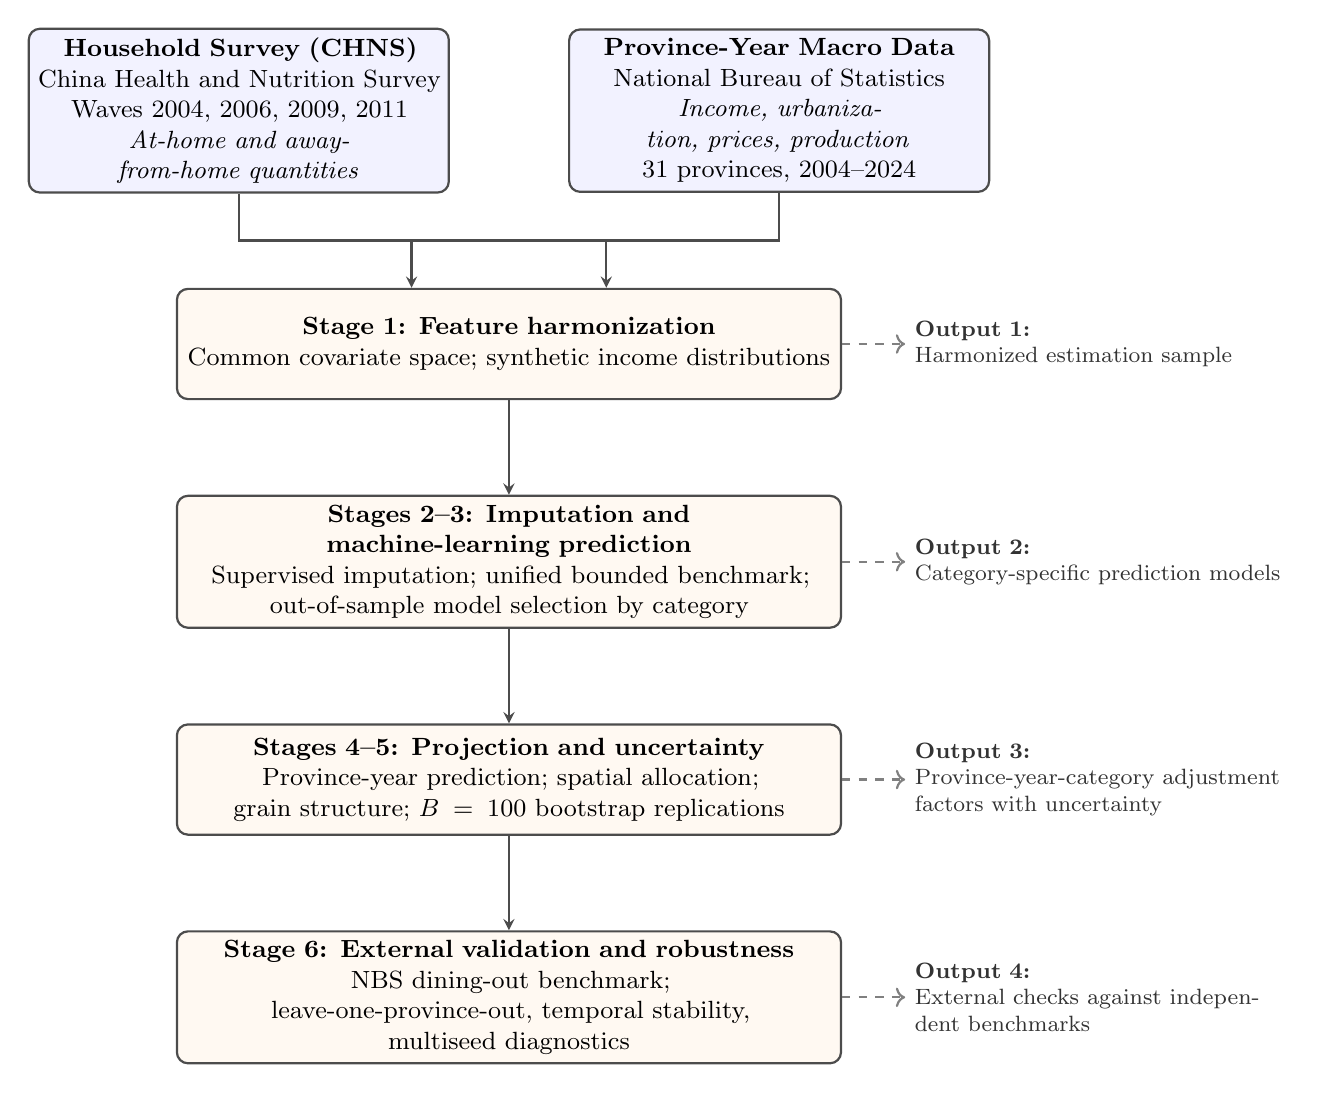
\begin{tikzpicture}[
    box/.style={draw=black!70, rounded corners=4pt, minimum height=1.4cm, align=center, thick, font=\small},
    inputBox/.style={box, fill=blue!5, text width=5.1cm},
    processBox/.style={box, fill=orange!5, text width=8.2cm},
    noteText/.style={text width=4.7cm, align=left, font=\footnotesize\color{black!80}},
    arrow/.style={->, >=stealth, thick, draw=black!70}
]
\node[inputBox] (micro) {%
  \textbf{Household Survey (CHNS)}\\
  China Health and Nutrition Survey\\
  Waves 2004, 2006, 2009, 2011\\
  \textit{At-home and away-from-home quantities}};
\node[inputBox, right=1.5cm of micro] (macro) {%
  \textbf{Province-Year Macro Data}\\
  National Bureau of Statistics\\
  \textit{Income, urbanization, prices, production}\\
  31 provinces, 2004--2024};
\coordinate (mid) at ($(micro.south)!0.5!(macro.south)$);
\node[processBox, below=1.2cm of mid] (stage1) {%
  \textbf{Stage 1: Feature harmonization}\\
  Common covariate space; synthetic income distributions};
\node[processBox, below=1.2cm of stage1] (stage2) {%
  \textbf{Stages 2--3: Imputation and machine-learning prediction}\\
  Supervised imputation; unified bounded benchmark;\\ out-of-sample model selection by category};
\node[processBox, below=1.2cm of stage2] (stage3) {%
  \textbf{Stages 4--5: Projection and uncertainty}\\
  Province-year prediction; spatial allocation;\\ grain structure; $B=100$ bootstrap replications};
\node[processBox, below=1.2cm of stage3] (stage4) {%
  \textbf{Stage 6: External validation and robustness}\\
  NBS dining-out benchmark;\\ leave-one-province-out, temporal stability,\\ multiseed diagnostics};
\node[noteText, right=0.8cm of stage1] (out1) {%
  \textbf{Output 1:}\\Harmonized estimation sample};
\node[noteText, right=0.8cm of stage2] (out2) {%
  \textbf{Output 2:}\\Category-specific prediction models};
\node[noteText, right=0.8cm of stage3] (out3) {%
  \textbf{Output 3:}\\Province-year-category adjustment factors with uncertainty};
\node[noteText, right=0.8cm of stage4] (out4) {%
  \textbf{Output 4:}\\External checks against independent benchmarks};
\draw[arrow] (micro.south)  |- ($(stage1.north)+(0,0.6cm)$) -| (stage1.150);
\draw[arrow] (macro.south)  |- ($(stage1.north)+(0,0.6cm)$) -| (stage1.30);
\draw[arrow] (stage1.south) -- (stage2.north);
\draw[arrow] (stage2.south) -- (stage3.north);
\draw[arrow] (stage3.south) -- (stage4.north);
\draw[->, dashed, draw=black!50, thick] (stage1.east) -- (out1.west);
\draw[->, dashed, draw=black!50, thick] (stage2.east) -- (out2.west);
\draw[->, dashed, draw=black!50, thick] (stage3.east) -- (out3.west);
\draw[->, dashed, draw=black!50, thick] (stage4.east) -- (out4.west);
\end{tikzpicture}%
}
\caption{Empirical workflow for estimating province-year-category food-away-from-home (FAFH) adjustment factors. CHNS = China Health and Nutrition Survey; NBS = National Bureau of Statistics of China. Stage 6 checks the projected factors against NBS urban-household dining-out (\textit{zaiwai yongcan}) expenditure, leave-one-province-out spatial extrapolation, a drop-last-wave temporal-stability diagnostic, and multiseed re-estimation of the preferred estimator.}
\label{fig:workflow}
\end{figure}

\subsection{Model families}

Predictive measurement requires a benchmark that is broad enough to test whether the results depend on model flexibility but structured enough to be interpretable. We therefore compare four model families (Table~\ref{tab:model_families}). Fractional logit is included as the bounded econometric benchmark. Regularized linear models establish the performance of parsimonious linear approximations. Tree ensembles test whether nonlinearities and interactions improve prediction in tabular data. Deep tabular networks test whether feature-token interactions add further predictive value.

\begin{table}[htbp]
\centering
\small
\caption{Model families in the unified benchmark}
\label{tab:model_families}
\begin{threeparttable}
\begin{tabularx}{\textwidth}{p{2.6cm} p{3.5cm} X}
\toprule
Family & Models & Rationale for inclusion \\
\midrule
Fractional response & Fractional logit & Econometric benchmark for a bounded outcome. It imposes a logistic conditional mean and respects the unit interval, but allows less flexible interactions than tree or deep models. \\ \addlinespace
Regularized linear & Ridge, Lasso & Transparent benchmarks that test whether a linear relationship, with shrinkage to limit overfitting, is sufficient for predicting the at-home ratio. \\ \addlinespace
Tree-based ensembles & Random Forest, XGBoost, LightGBM, CatBoost & Strong competitors for small- and medium-sized tabular data. They capture nonlinearities and interactions without requiring prespecified functional forms. \\ \addlinespace
Deep tabular networks & Multilayer perceptron (MLP), Tabular ResNet, FT-Transformer, TabM & Neural-network architectures for tabular data. The FT-Transformer tokenizes features and uses attention to learn interactions among income, province, prices, production, and food-service indicators. \\
\bottomrule
\end{tabularx}
\begin{tablenotes}[flushleft]
\scriptsize
\item Notes: XGBoost = Extreme Gradient Boosting; LightGBM = Light Gradient Boosting Machine; ResNet = residual neural network; FT-Transformer = feature-tokenizer transformer. The model comparison is used for estimator selection only; the final province-year estimates use the full projection pipeline.
\end{tablenotes}
\end{threeparttable}
\end{table}

\subsection{Candidate estimators}

All candidates are implemented under a common protocol. Fractional logit estimates a logistic conditional mean for the bounded ratio by quasi-maximum likelihood \citep{PapkeWooldridge1996}; ridge and lasso provide penalized linear baselines \citep{Hoerl1970Ridge, Tibshirani1996}; the tree ensembles (Random Forest, XGBoost, LightGBM, CatBoost) approximate the conditional mean as additive collections of regression trees \citep{Breiman2001, ChenGuestrin2016, KeEtAl2017, ProkhorenkovaEtAl2018}; and the deep tabular networks (MLP, Tabular ResNet, FT-Transformer, TabM) learn feature representations directly \citep{GoodfellowEtAl2016, GorishniyEtAl2021, RubachevEtAl2024}. The FT-Transformer assigns each numerical or categorical feature its own token and applies self-attention across tokens, so interactions among household income, province, urbanization, prices, production structure, and food-service indicators are learned rather than prespecified; a sigmoid output layer keeps predictions on the unit interval. The baseline configuration uses three encoder layers, 64-dimensional tokens, four attention heads, dropout of 0.1, AdamW optimization, and early stopping. Appendix~\ref{app:estimators} states the estimating equations for each family.

\subsection{Tuning, imputation, spatial allocation, and uncertainty}

All models are tuned on validation data that are disjoint from the test folds. Regularized linear penalties are selected by fivefold cross-validation on the training portion of each fold. Tree ensembles tune tree depth or leaves, number of trees, learning rate, and subsampling rates. Deep tabular networks tune depth, hidden dimension, and dropout. Because neural-network training can be seed-sensitive, Section~\ref{subsec:seeds} reports FT-Transformer performance across five seeds.

Some CHNS households report total consumption but not the FAH/FAFH split for a category. We impute missing at-home ratios using supervised models trained on complete observations in the same wave. The imputation stage uses the same menu of candidate models and selects the lowest fivefold cross-validation mean absolute error (MAE) by category. Appendix Table~\ref{tab:imputation} reports the imputation-stage performance. A no-imputation specification is reported in Section~\ref{subsec:robust} to verify that the headline findings do not depend on this step.

National reporting requires coverage of all 31 provincial units. For provinces not directly represented in the CHNS, the fitted model predicts from province-year covariates and a deterministic allocation step preserves three constraints. Provincial adjustment-factor predictions are bounded above by $1/\varepsilon$. Within the four staple-grain categories, shares are normalized to sum to one. For cells with weak direct support, inverse-distance weighting smooths predictions among provinces with similar covariate profiles \citep{Shepard1968}. This step affects only a small number of cells but stabilizes upper-tail provincial predictions.

We report two forms of uncertainty. Sampling uncertainty is captured by a household-level percentile bootstrap with $B=100$ replicates \citep{Efron1993}. In each replicate, imputation, prediction, spatial allocation, and grain-structure steps are re-executed; the reported 95\% interval is the corresponding percentile interval. Model uncertainty is reported separately as the spread across plausible specifications. We keep these two sources separate because the bootstrap is conditional on the chosen specification, whereas model spread reflects sensitivity to modeling choices. Combining them mechanically would require additional distributional assumptions that are not justified by the available data.

\subsection{Unified benchmark design}

The benchmark used for model selection is intentionally narrower than the full projection pipeline. Within each food category, all candidate models use the same predictors, the same five time-aware folds, and the same bounded postprediction rule. The benchmark records both ratio-scale and AF-scale metrics. Ratio-scale metrics evaluate the bounded target directly. AF-scale metrics answer the practical question: how much should FAH quantities be scaled to recover total consumption? The province-year estimates reported below are generated after model selection by the full FT-Transformer pipeline, including imputation, spatial allocation, and bootstrap uncertainty.

% =====================================================================
\section{Adjustment-factor estimates}
\label{sec:results}

The results proceed from model selection to the adjustment factors themselves. We first establish which estimator most reliably predicts the bounded at-home ratio under a common validation design. We then report national factors, provincial heterogeneity, and robustness across alternative specifications. Each result is interpreted in relation to the paper's measurement question: how much FAH quantities should be scaled to approximate total consumption.

\subsection{Model comparison under the bounded benchmark}
\label{subsec:benchmark}

The unified benchmark asks which model best predicts the household at-home ratio when all candidates use the same folds, features, and postprediction bounds. FT-Transformer ranks first on both the ratio scale and the AF scale (Table~\ref{tab:benchmark}). Its advantage over Tabular ResNet, Lasso, CatBoost, LightGBM, and Random Forest is moderate rather than overwhelming. This pattern matters for interpretation: the preferred model is supported empirically, but the substantive conclusion that FAH quantities understate total consumption does not depend on a single algorithm.

\begin{table}[htbp]
\centering
\small
\begin{threeparttable}
\caption{Unified bounded benchmark of prediction accuracy}
\label{tab:benchmark}
\begin{tabular*}{\textwidth}{@{\extracolsep{\fill}} l l cccc @{}}
\toprule
Rank & Model & Ratio MAE & Ratio RMSE & AF MAE & AF RMSE \\
\midrule
1 & FT-Transformer & 0.067 & 0.151 & 0.203 & 1.078 \\
2 & Tabular ResNet & 0.076 & 0.154 & 0.217 & 1.099 \\
3 & Lasso          & 0.087 & 0.153 & 0.231 & 1.098 \\
4 & CatBoost       & 0.090 & 0.155 & 0.235 & 1.079 \\
5 & LightGBM       & 0.092 & 0.155 & 0.236 & 1.071 \\
6 & Random Forest  & 0.094 & 0.157 & 0.239 & 1.076 \\
7 & XGBoost        & 0.105 & 0.179 & 0.291 & 1.219 \\
8 & MLP            & 0.114 & 0.193 & 0.292 & 1.122 \\
9 & Ridge          & 0.091 & 0.165 & 0.372 & 1.371 \\
\addlinespace
-- & Fractional logit & 0.113 & 0.164 & 0.338 & 2.772 \\
\bottomrule
\end{tabular*}
\begin{tablenotes}[flushleft]
\scriptsize
\item Notes: All models are evaluated on identical fivefold, time-aware splits using the same feature set. Predictions of the at-home ratio are bounded to $(\varepsilon,1-\varepsilon)$ with $\varepsilon=0.02$ before reciprocal conversion to the adjustment-factor (AF) scale. MAE = mean absolute error; RMSE = root mean squared error; MLP = multilayer perceptron; ResNet = residual neural network; XGBoost = Extreme Gradient Boosting; LightGBM = Light Gradient Boosting Machine. The benchmark is used only for model selection; reported estimates are generated by the full FT-Transformer projection pipeline.
\end{tablenotes}
\end{threeparttable}
\end{table}

\subsection{National adjustment factors}
\label{subsec:national}

The national estimates show the scale and composition of FAFH undermeasurement. All 2024 factors exceed one, meaning that FAH quantities alone understate total consumption for every reported category (Table~\ref{tab:national}). The smallest factor is for dairy (1.099), followed by fruits (1.117) and eggs (1.126). The largest factor is for poultry (1.405), followed by beef (1.363), rice (1.276), pork (1.273), and aquatic products (1.267).

This ordering is consistent with how foods enter commercial eating channels. Poultry, beef, pork, and aquatic products are common in restaurants, canteens, and prepared-food meals, whereas dairy and eggs are more often acquired for household use. The estimates therefore imply that FAFH omission changes the measured composition of demand, not only its aggregate level. This has direct implications for protein-demand assessment, feed-demand projections, and food self-sufficiency analysis.

The time series in Figure~\ref{fig:national_panel} show that several factors rise during 2015--2024, especially poultry, rice, pork, and aquatic products. Beef, dairy, and eggs decline modestly. These are projection-based estimates from a relationship learned on CHNS data for 2004--2011, not direct survey measurements after 2011. The long projection window is therefore a source of uncertainty. Later in the paper, Section~\ref{sec:validation} evaluates the extent to which the relationship can be transported across space and time.

\begin{figure}[htbp]
\centering
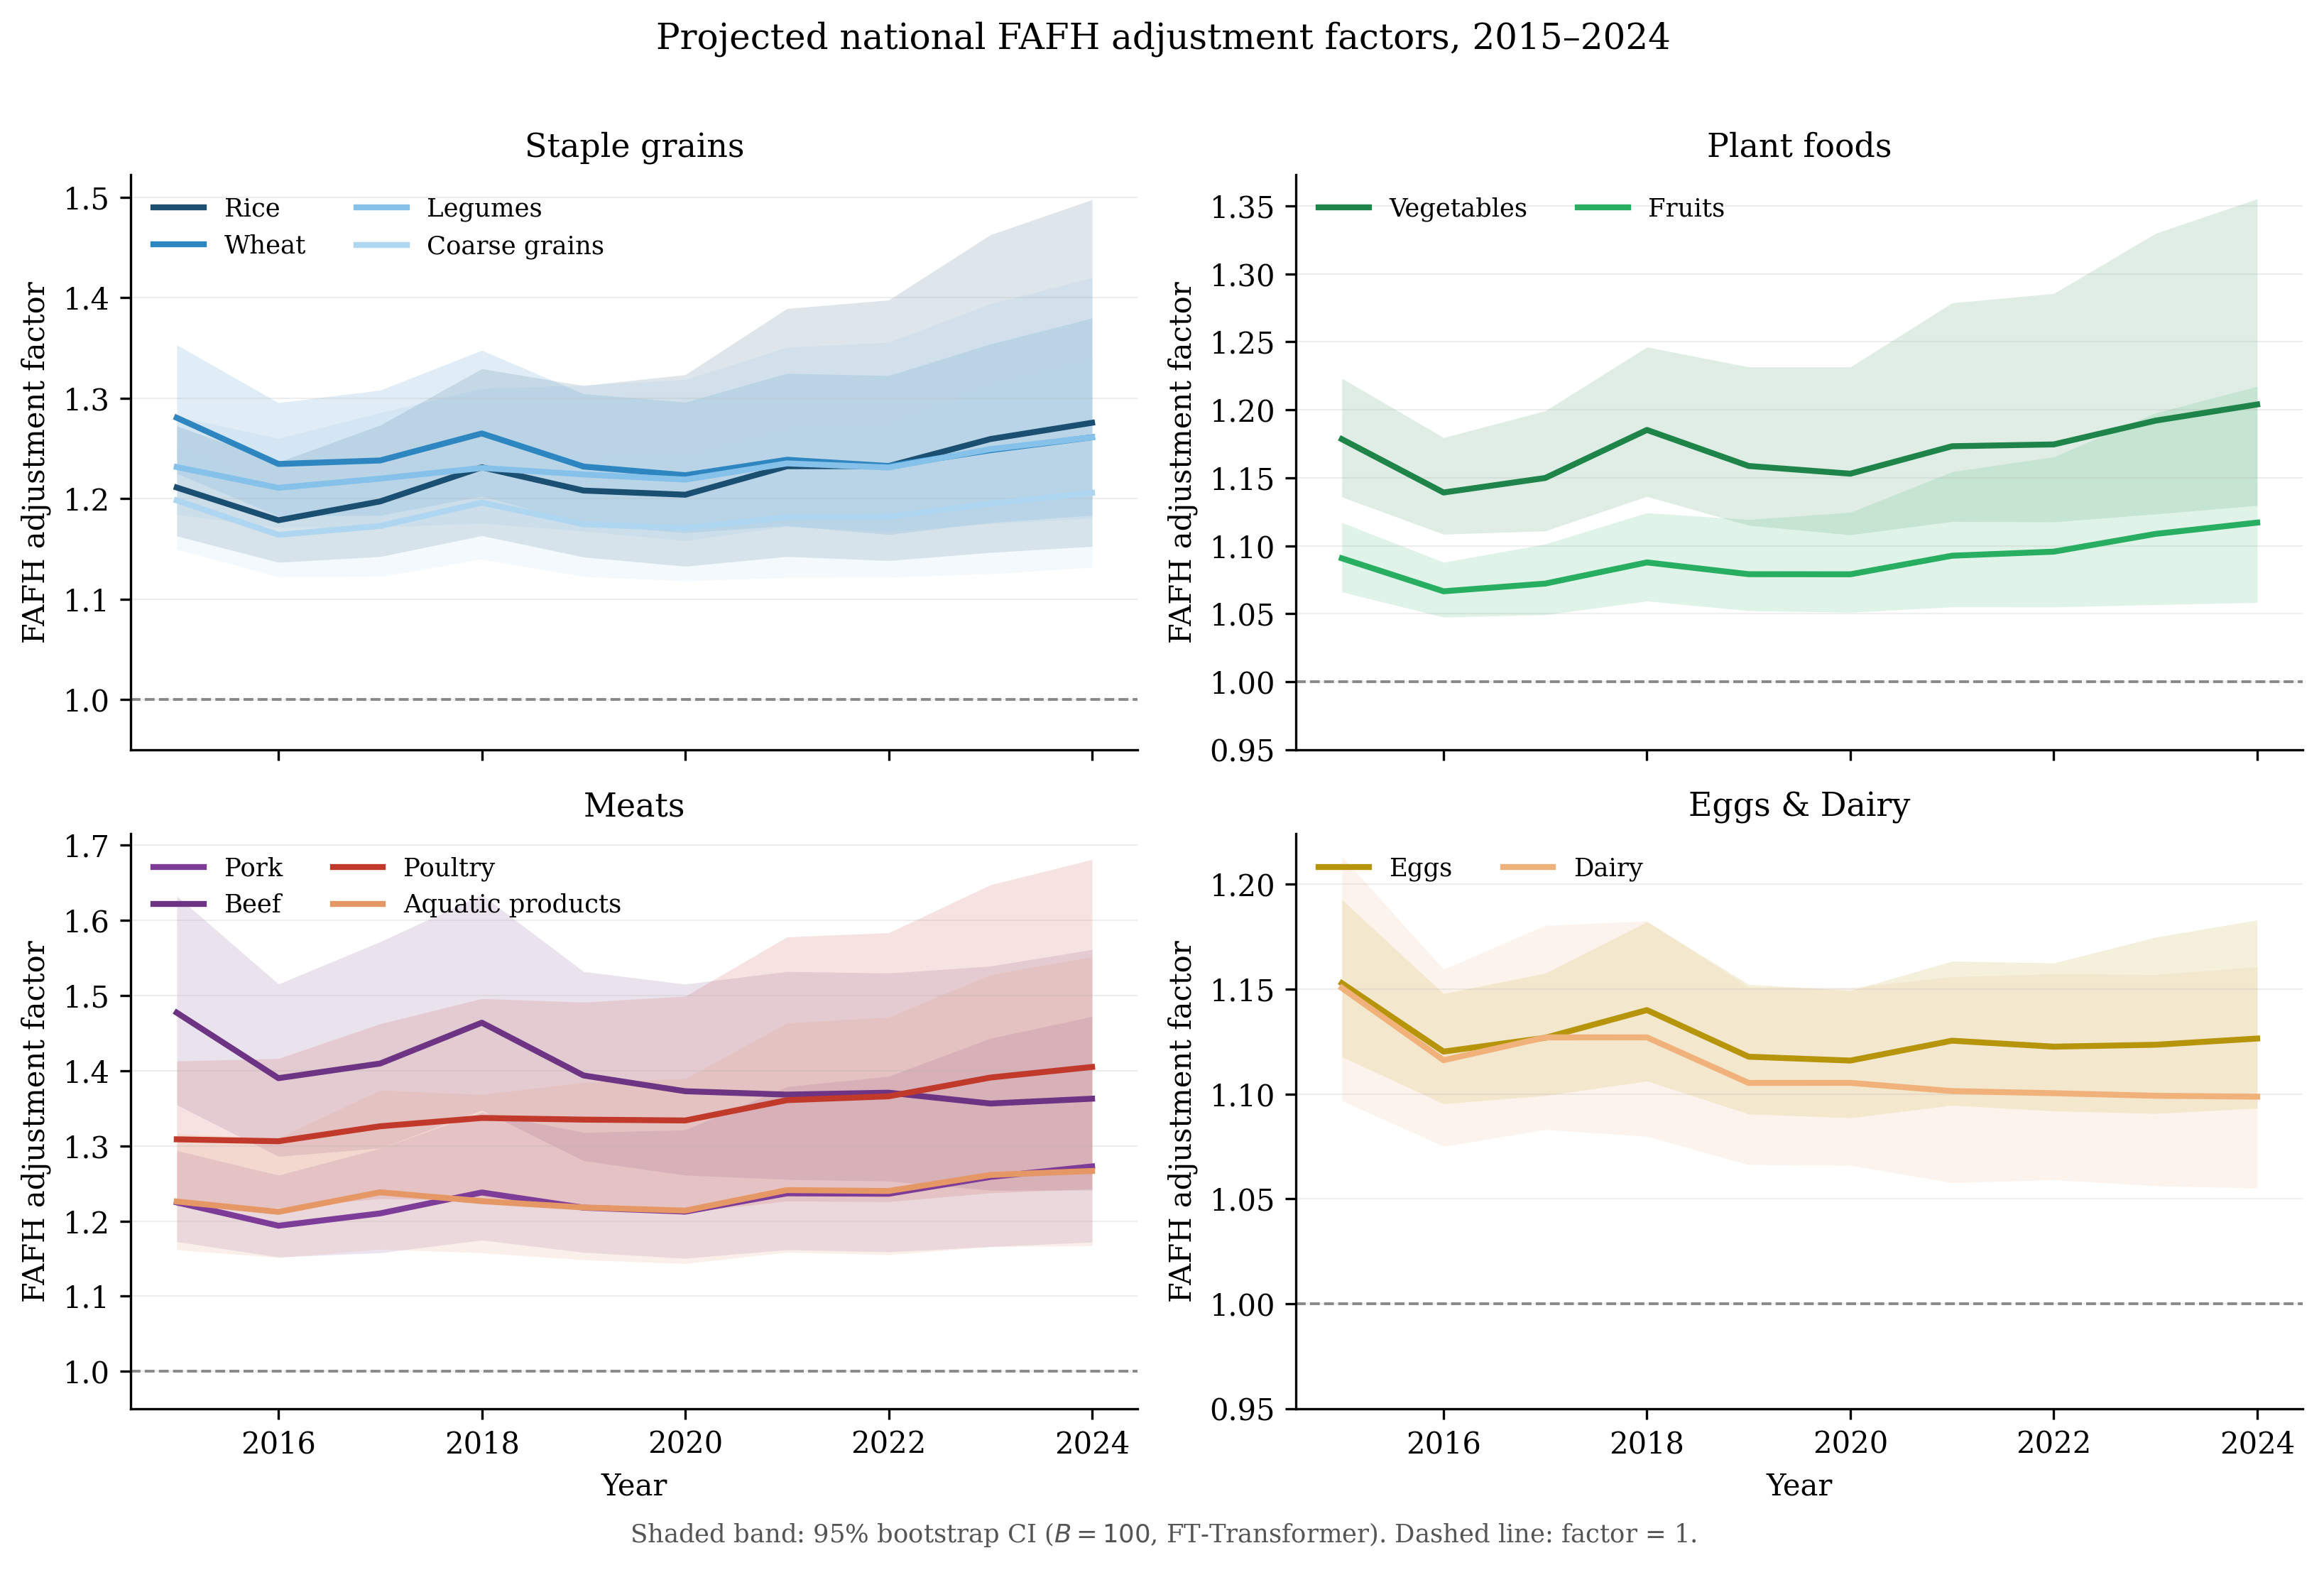
\includegraphics[width=1\linewidth]{fig2_national_panel_ci.png}
\caption{Projected national food-away-from-home (FAFH) adjustment factors by commodity group, 2015--2024. Solid lines are FT-Transformer point estimates. Shaded areas are 95\% household-level bootstrap intervals ($B=100$). The dashed horizontal line denotes an adjustment factor of one.}
\label{fig:national_panel}
\end{figure}

\begin{table}[htbp]
\centering
\caption{Projected national FAFH adjustment factors}
\label{tab:national}
\begin{threeparttable}
\small
\setlength{\tabcolsep}{0pt}
\begin{tabular*}{\textwidth}{@{\extracolsep{\fill}} l c c c c c @{}}
\toprule
Food category & 2015 & 2019 & 2024 & 95\% CI (2024) & Change, 2015--2024 \\
\midrule
Rice & 1.211 & 1.208 & 1.276 & (1.152, 1.498) & $+5.3\%$ \\
Wheat & 1.281 & 1.232 & 1.261 & (1.183, 1.380) & $-1.5\%$ \\
Legumes & 1.231 & 1.224 & 1.261 & (1.180, 1.420) & $+2.4\%$ \\
Coarse grains & 1.198 & 1.175 & 1.206 & (1.132, 1.338) & $+0.6\%$ \\
Vegetables & 1.178 & 1.159 & 1.204 & (1.130, 1.355) & $+2.2\%$ \\
Fruits & 1.091 & 1.079 & 1.117 & (1.058, 1.217) & $+2.4\%$ \\
Pork & 1.225 & 1.218 & 1.273 & (1.172, 1.472) & $+3.9\%$ \\
Beef & 1.477 & 1.394 & 1.363 & (1.241, 1.561) & $-7.7\%$ \\
Poultry & 1.309 & 1.335 & 1.405 & (1.243, 1.681) & $+7.4\%$ \\
Aquatic products & 1.226 & 1.218 & 1.267 & (1.167, 1.552) & $+3.3\%$ \\
Eggs & 1.153 & 1.118 & 1.126 & (1.093, 1.183) & $-2.3\%$ \\
Dairy & 1.150 & 1.105 & 1.099 & (1.055, 1.161) & $-4.5\%$ \\
\bottomrule
\end{tabular*}
\begin{tablenotes}[flushleft]
\scriptsize
\item Notes: Values are adjustment factors, defined as total consumption divided by food-at-home consumption. A value above one indicates that food-at-home quantities understate total demand. The 95\% confidence intervals (CIs) are percentile bootstrap intervals from the FT-Transformer projection pipeline with $B=100$ household-level resamples. The factors are intended for converting secondary food-at-home quantity data into approximate total-consumption quantities. Intervals capture sampling uncertainty conditional on the baseline specification; cross-specification uncertainty is reported in Section~\ref{subsec:robust}.
\end{tablenotes}
\end{threeparttable}
\end{table}

Figure~\ref{fig:dotwhisker} summarizes the 2024 national estimates and intervals. The compositional message is clear: poultry and beef require the largest corrections, while dairy, fruits, and eggs require the smallest. Wider intervals for poultry, aquatic products, and rice reflect greater heterogeneity in FAFH behavior and weaker precision for those categories.

\begin{figure}[htbp]
\centering
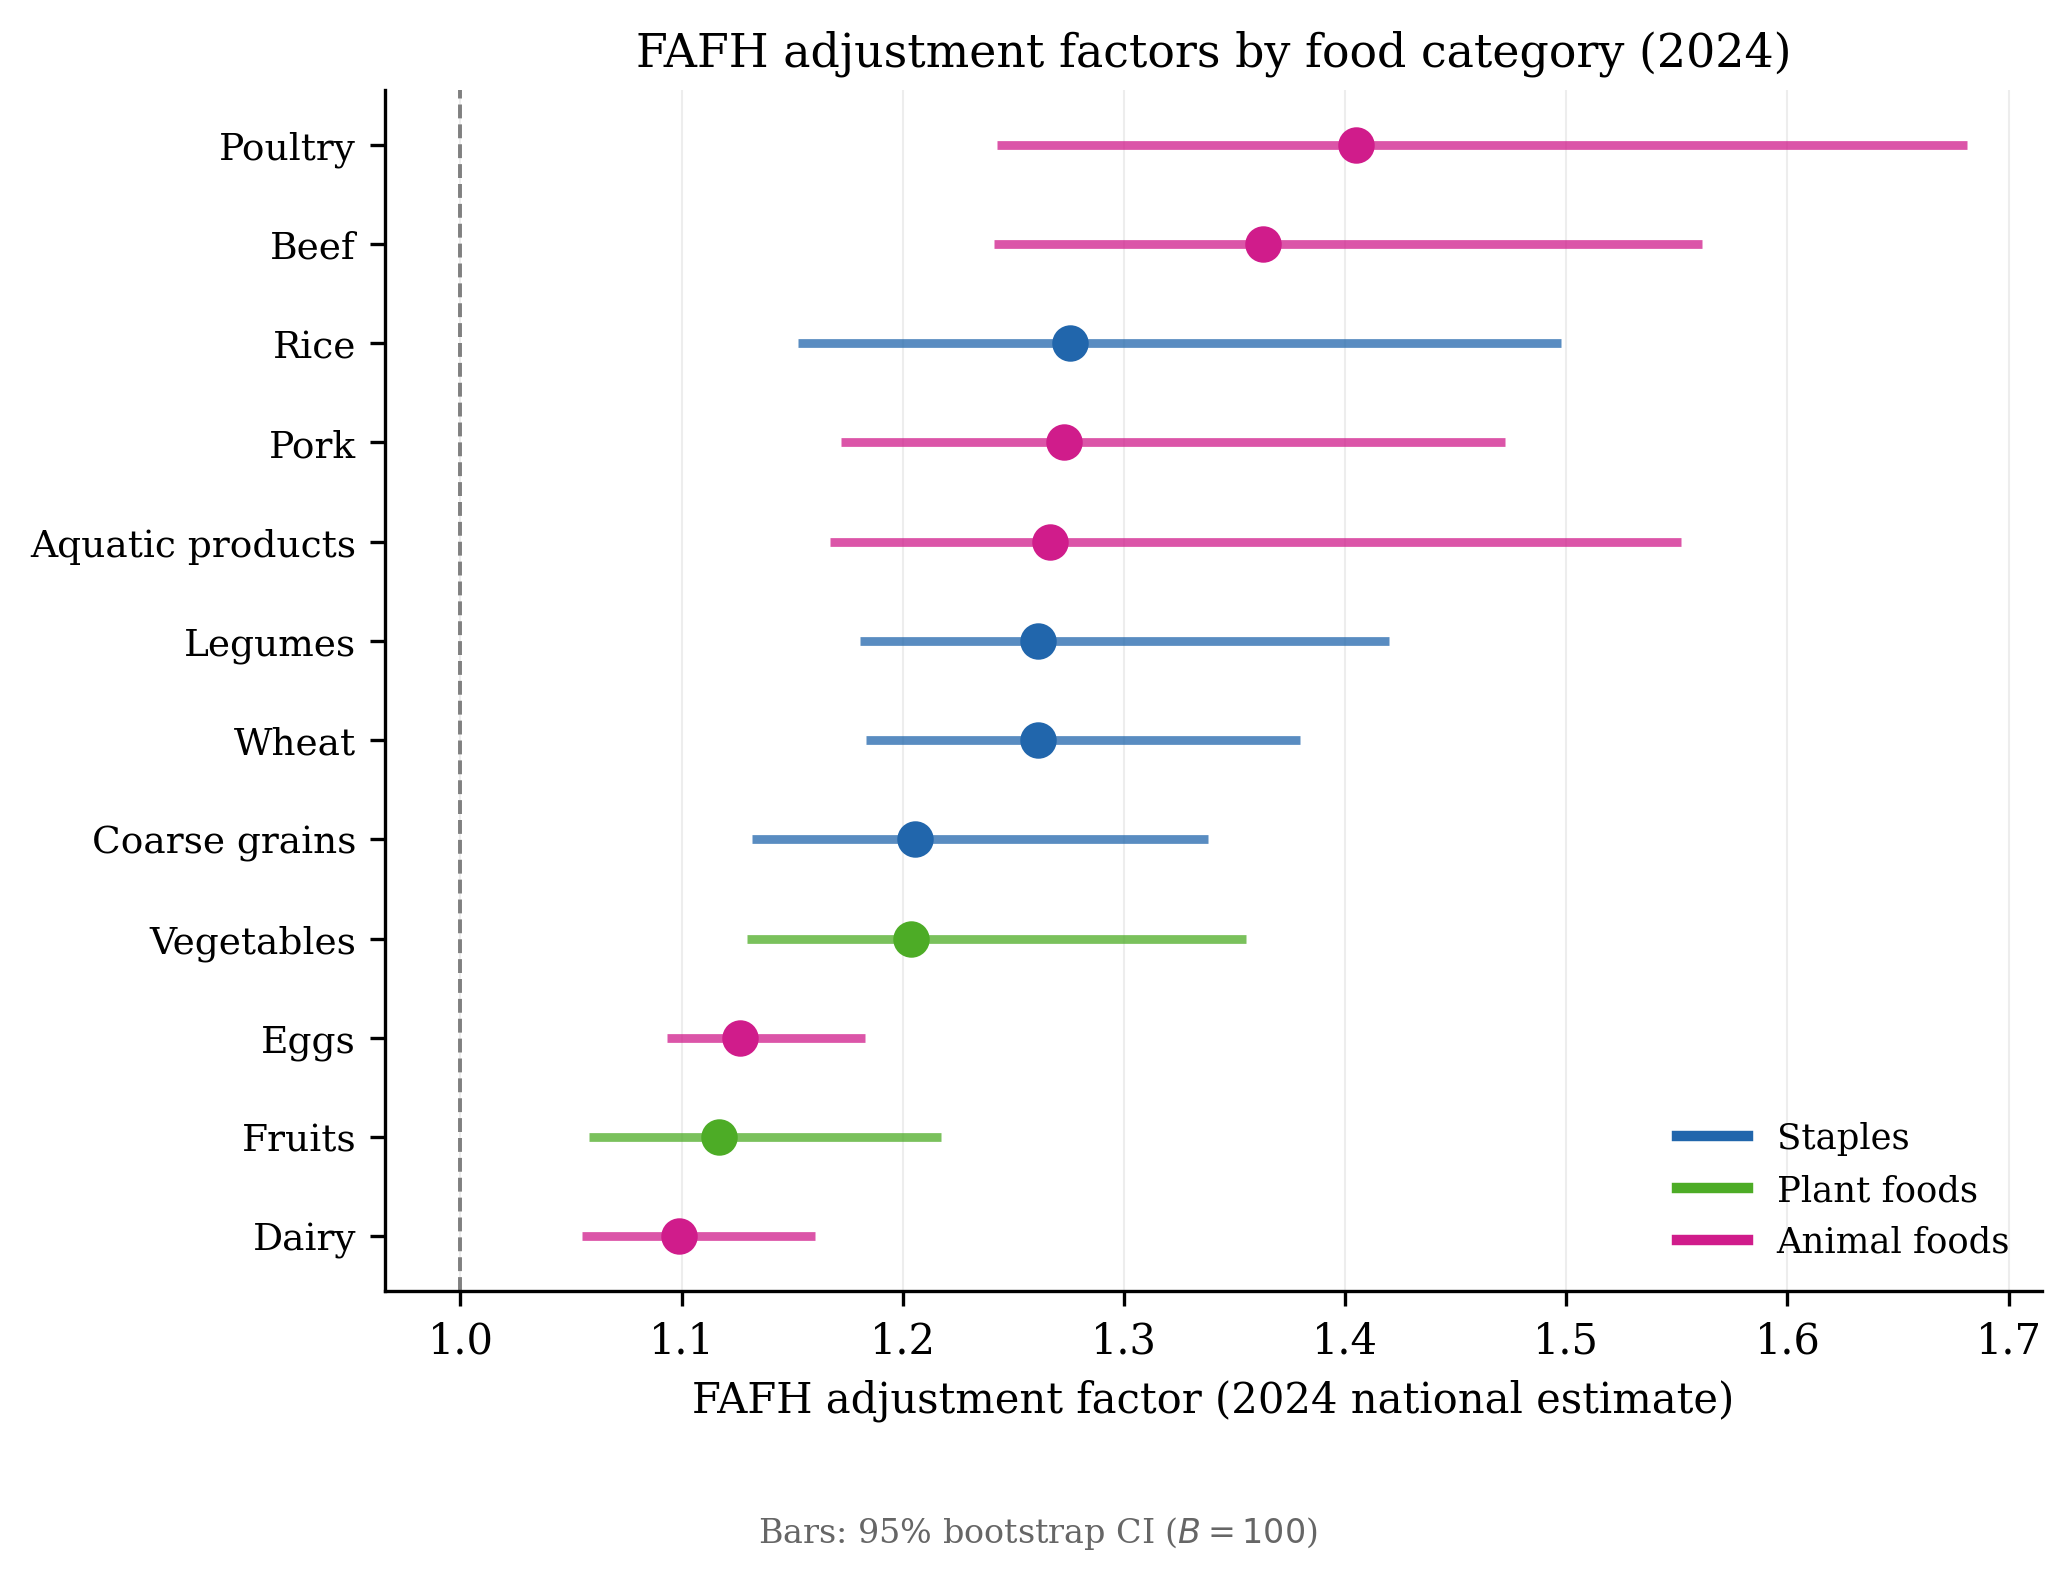
\includegraphics[width=0.95\linewidth]{fig3_dotwhisker_2024.png}
\caption{National food-away-from-home (FAFH) adjustment factors by food category in 2024. Points are FT-Transformer estimates; horizontal bars are 95\% bootstrap intervals ($B=100$). The dashed vertical line marks an adjustment factor of one.}
\label{fig:dotwhisker}
\end{figure}

\subsection{Provincial heterogeneity}
\label{subsec:provincial}

The provincial estimates show that a single national multiplier is insufficient for regional analysis. Table~\ref{tab:provincial} reports all nine core CHNS provinces, two metropolitan oversamples, one high-income coastal province included for comparison, and the population-weighted national average. Metropolitan and coastal provinces have higher adjustment factors than most inland provinces. Shanghai and Beijing are above the national average for all four displayed categories, while Henan, Hubei, Hunan, Heilongjiang, and Liaoning are below the national average for most categories.

These differences are consistent with variation in income, urbanization, and food-service development. They also show why province-specific multipliers matter. Applying a single national factor would overstate consumption in some lower-FAFH provinces and understate consumption in metropolitan food-service markets. At the same time, the table should not be read as evidence for fine subprovincial inference: Beijing and Shanghai are observed only in 2011, Zhejiang is projected from covariates, and several provinces outside the CHNS support rely entirely on projection.

\begin{table}[htbp]
\centering
\begin{threeparttable}
\caption{Provincial adjustment factors for selected categories, 2024}
\label{tab:provincial}
\small
\setlength{\tabcolsep}{6pt}
\renewcommand{\arraystretch}{1.1}
\begin{tabular*}{\textwidth}{@{\extracolsep{\fill}} ll cccc @{}}
\toprule
Province & Type\textsuperscript{a} & Rice & Vegetables & Pork & Aquatic products \\
\midrule
Beijing       & Metro & 1.500 & 1.344 & 1.451 & 1.515 \\
Shanghai      & Metro & 1.533 & 1.377 & 1.492 & 1.528 \\
Zhejiang      & OOS   & 1.371 & 1.275 & 1.364 & 1.348 \\
Liaoning      & IS    & 1.193 & 1.161 & 1.183 & 1.195 \\
Heilongjiang  & IS    & 1.197 & 1.169 & 1.187 & 1.201 \\
Jiangsu       & IS    & 1.235 & 1.135 & 1.257 & 1.245 \\
Shandong      & IS    & 1.251 & 1.142 & 1.270 & 1.255 \\
Henan         & IS    & 1.163 & 1.117 & 1.204 & 1.189 \\
Hubei         & IS    & 1.184 & 1.127 & 1.222 & 1.214 \\
Hunan         & IS    & 1.175 & 1.120 & 1.214 & 1.207 \\
Guangxi       & IS    & 1.230 & 1.150 & 1.213 & 1.224 \\
Guizhou       & IS    & 1.205 & 1.126 & 1.184 & 1.329 \\
\midrule
National avg. & ---   & 1.276 & 1.204 & 1.273 & 1.267 \\
\bottomrule
\end{tabular*}
\begin{tablenotes}[flushleft]
\scriptsize
\item[a] IS = in-sample province observed in all four CHNS waves. Metro = Beijing or Shanghai, which enter CHNS only in 2011. OOS = out-of-sample province estimated by projection from province-year covariates. National average is population-weighted across all 31 provinces. The full 31-province table for these four representative categories is reported in Appendix Table~\ref{tab:prov2024_full}. OOS and Metro estimates should be interpreted with additional extrapolation uncertainty, as illustrated by the leave-one-province-out diagnostic in Section~\ref{subsec:lopo}.
\end{tablenotes}
\end{threeparttable}
\end{table}

Figures~\ref{fig:map_mean} and \ref{fig:map_width} map the 2024 provincial estimates and uncertainty for the same four categories. High adjustment factors are concentrated in metropolitan and coastal provinces, while interval widths are wider for categories and provinces with weaker survey support. Figure~\ref{fig:province_box} summarizes the cross-province distribution across all reported categories; dispersion is especially large for animal-source foods.

\begin{figure}[htbp]
\centering
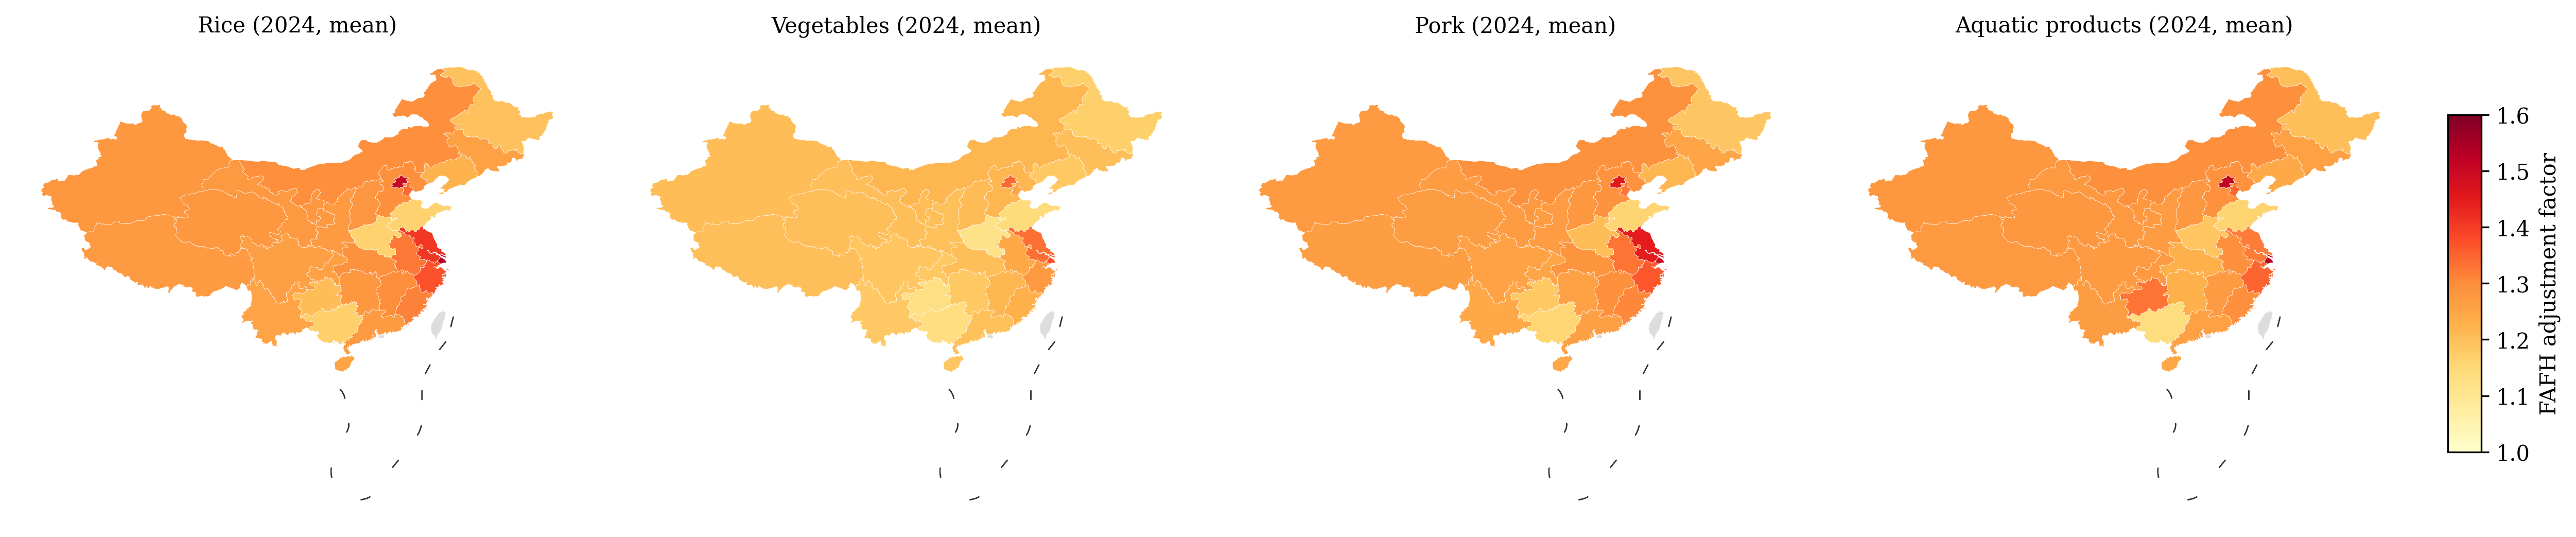
\includegraphics[width=1\linewidth]{fig4_map_mean_2024.png}
\caption{Province-level food-away-from-home (FAFH) adjustment factors in 2024 for selected categories. Darker colors indicate larger adjustment factors.}
\label{fig:map_mean}
\end{figure}

\begin{figure}[htbp]
\centering
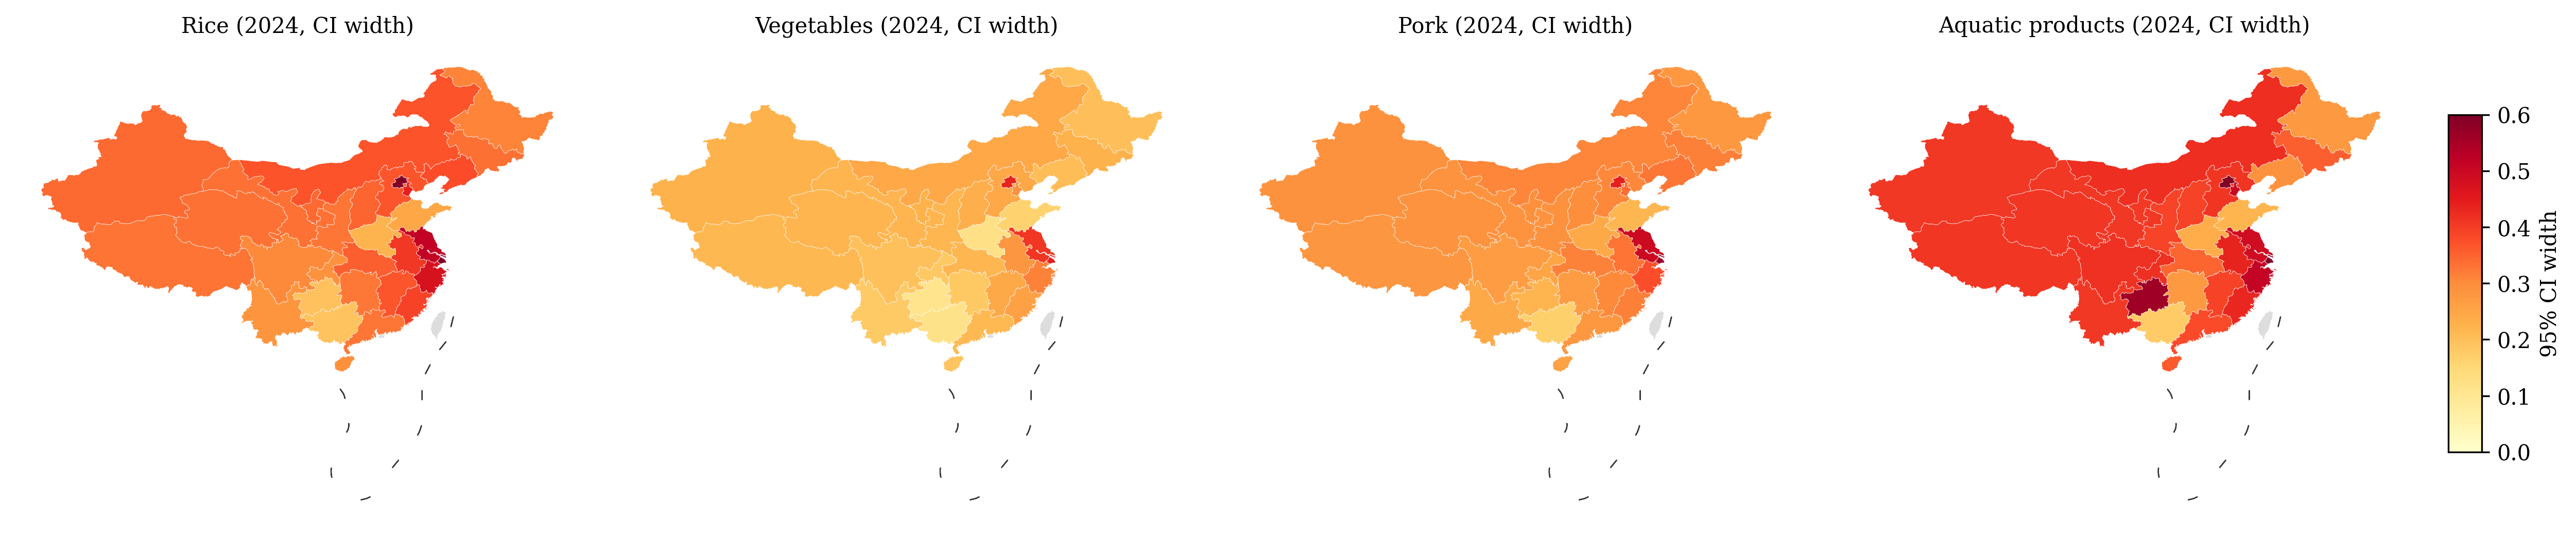
\includegraphics[width=1\linewidth]{fig4_map_width_2024.png}
\caption{Province-level width of 95\% bootstrap intervals in 2024 for selected categories. Darker colors indicate wider uncertainty intervals.}
\label{fig:map_width}
\end{figure}

\begin{figure}[htbp]
\centering
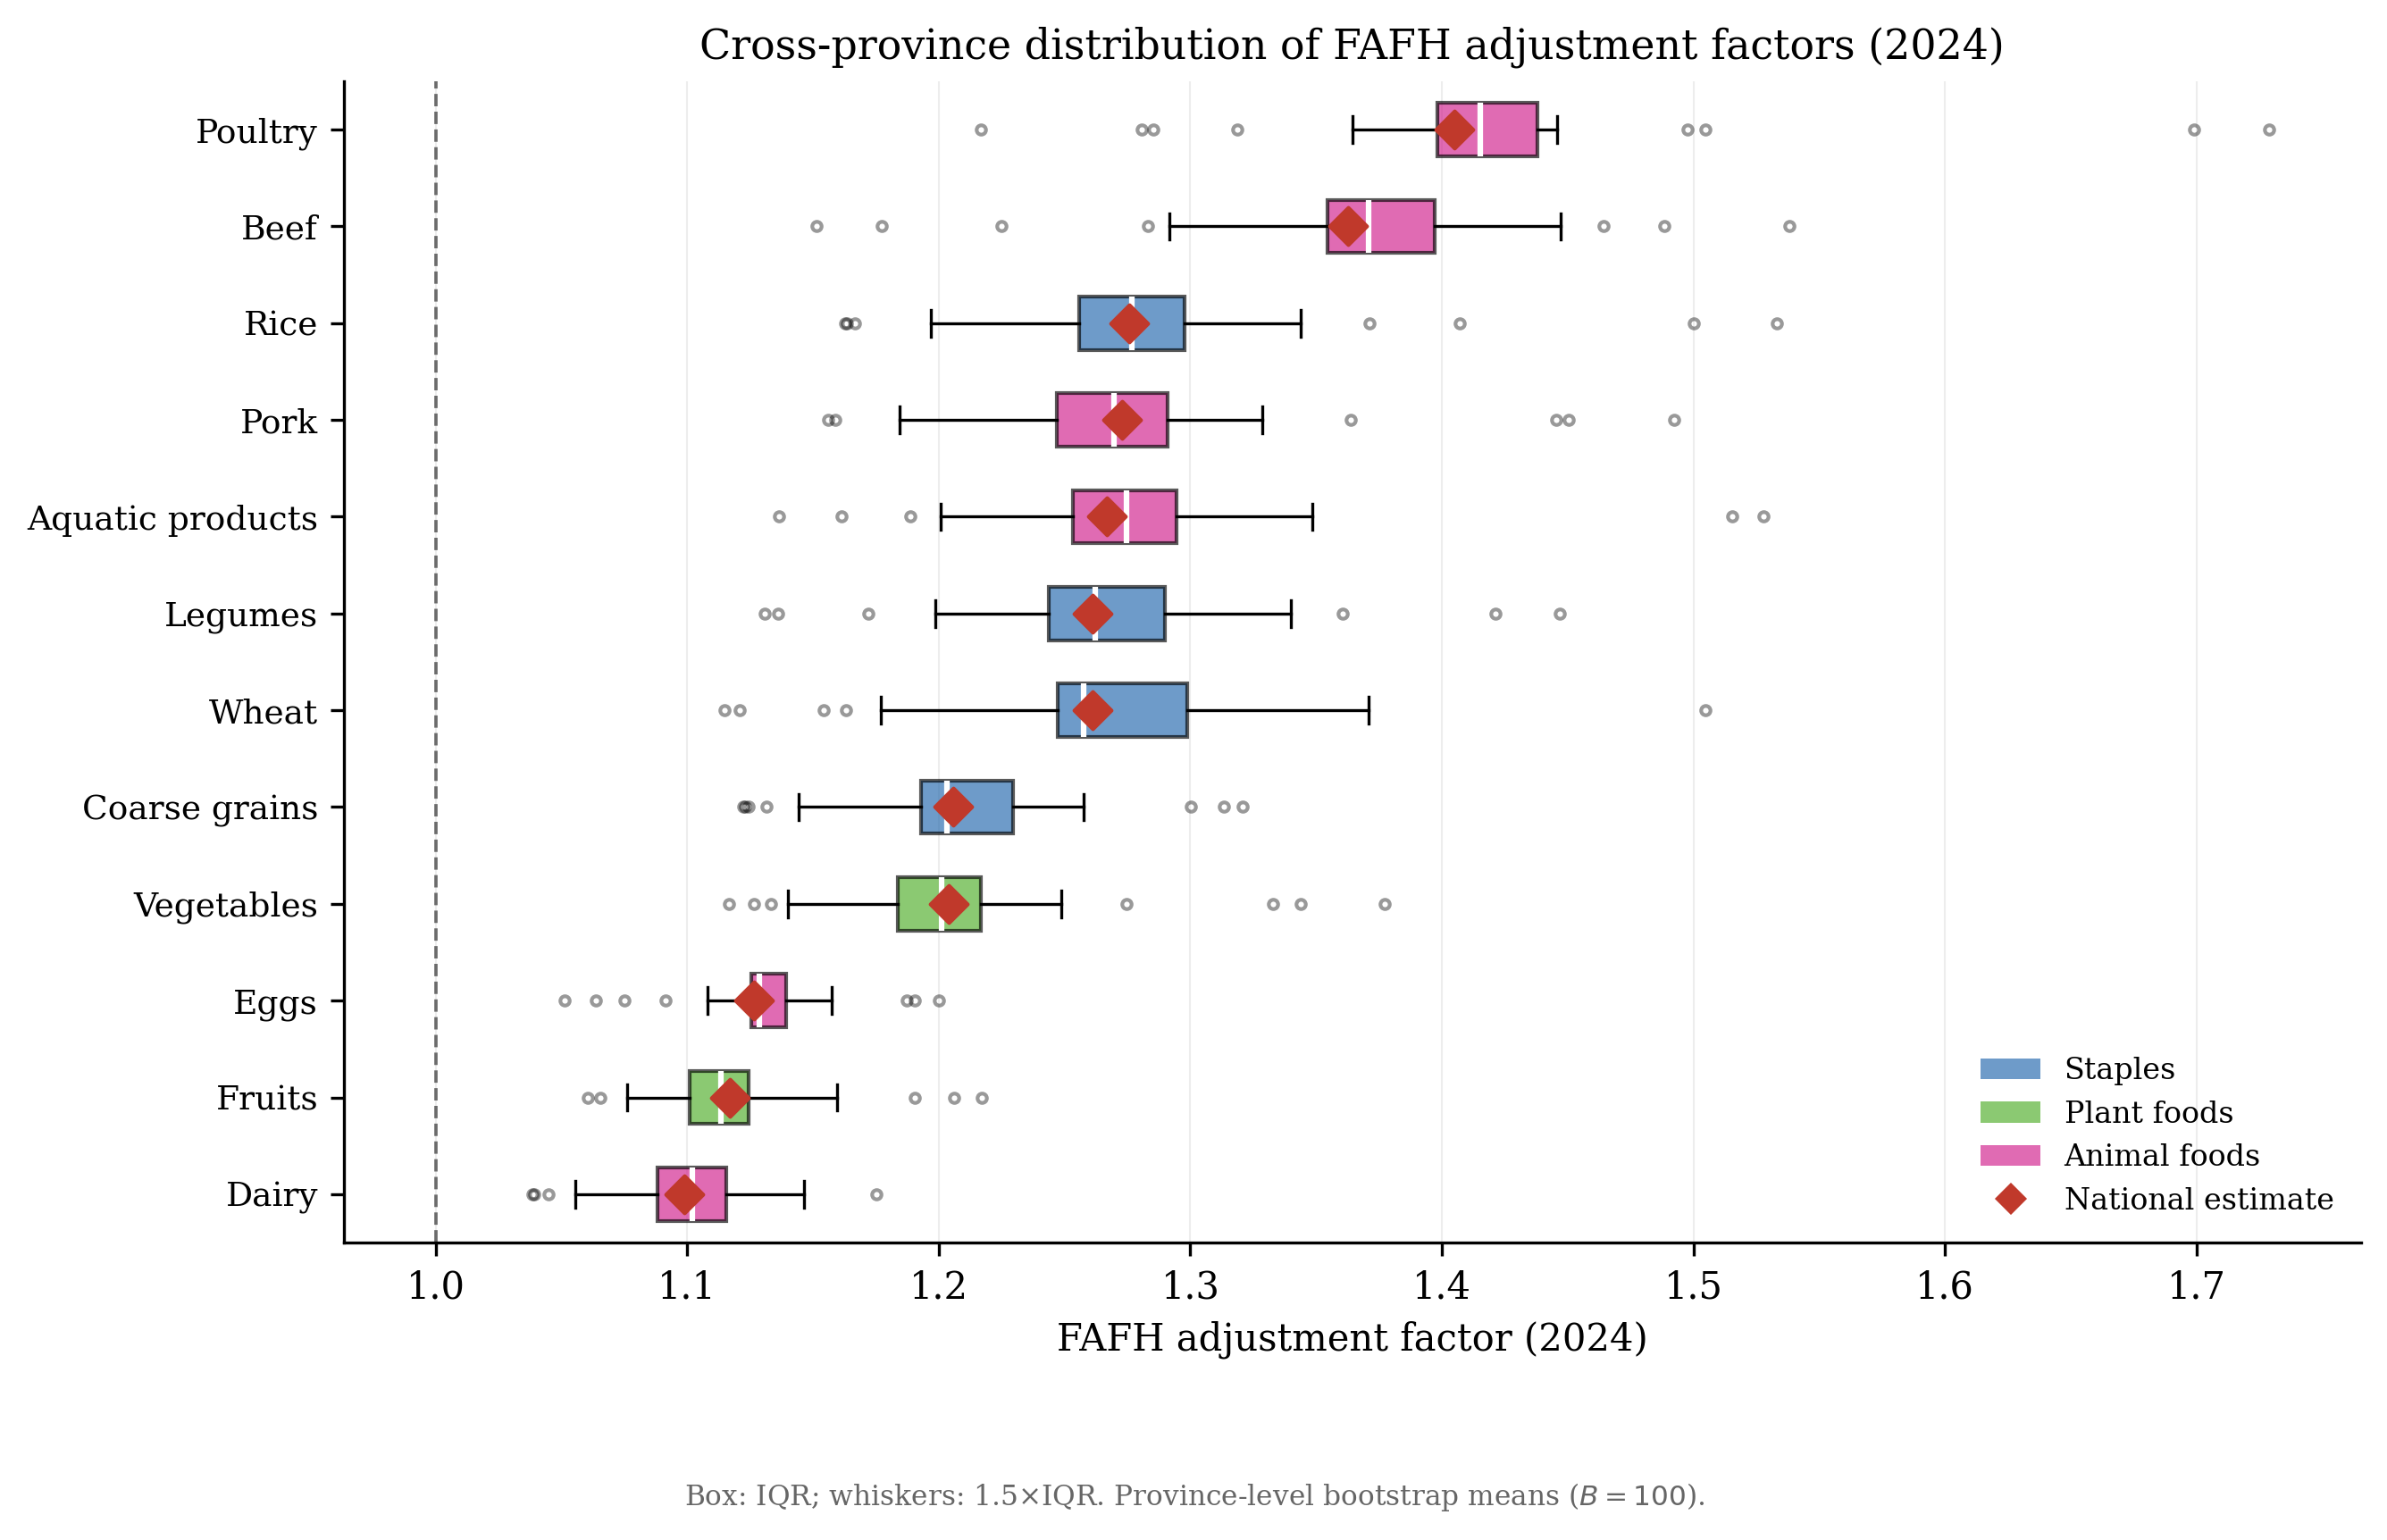
\includegraphics[width=1\linewidth]{fig5_province_boxplot_2024.png}
\caption{Cross-province distribution of food-away-from-home (FAFH) adjustment factors in 2024. Boxes show the interquartile range, whiskers extend to 1.5 times the interquartile range, and red diamonds report national estimates.}
\label{fig:province_box}
\end{figure}

\subsection{Robustness across specifications}
\label{subsec:robust}

The robustness exercise asks whether the substantive conclusions survive plausible alternative modeling choices. Table~\ref{tab:robustness} compares the 2024 national estimates with LightGBM, Random Forest, and a no-imputation FT-Transformer specification. All specifications produce factors above one for all categories, and the low-adjustment categories remain broadly the same. Beef and legumes are most sensitive to model choice, largely because the Random Forest specification yields substantially higher values. Wheat, eggs, fruits, and dairy are relatively stable.

This exercise highlights the distinction between sampling uncertainty and model uncertainty. Bootstrap intervals summarize uncertainty conditional on the baseline specification. The cross-model spread captures sensitivity to plausible modeling choices. For applied use, both should be considered when a category is central to the policy question. Additional appendix checks show that alternative-specification trajectories and sensitivity to the bounding parameter do not alter the main ordering of categories.

\begin{table}[htbp]
\centering
\small
\begin{threeparttable}
\caption{Robustness of national adjustment factors for 2024 across alternative specifications}
\label{tab:robustness}
\setlength{\tabcolsep}{0pt} 
\begin{tabular*}{\textwidth}{@{\extracolsep{\fill}} l ccccc @{}}
\toprule
Food category & Baseline & LightGBM & Random Forest & No imputation & Max abs. dev. \\
\midrule
Rice             & 1.276 & 1.072 & 1.098 & 1.187 & 0.203 \\
Wheat            & 1.261 & 1.207 & 1.258 & 1.245 & 0.054 \\
Legumes          & 1.261 & 1.232 & 1.742 & 1.307 & 0.481 \\
Coarse grains    & 1.206 & 1.113 & 1.098 & 1.145 & 0.107 \\
Vegetables       & 1.204 & 1.064 & 1.102 & 1.188 & 0.140 \\
Fruits           & 1.117 & 1.057 & 1.061 & 1.194 & 0.077 \\
Pork             & 1.273 & 1.221 & 1.268 & 1.366 & 0.093 \\
Beef             & 1.363 & 1.324 & 1.928 & 1.329 & 0.565 \\
Poultry          & 1.405 & 1.237 & 1.205 & 1.342 & 0.200 \\
Aquatic products & 1.267 & 1.202 & 1.398 & 1.462 & 0.195 \\
Eggs             & 1.126 & 1.067 & 1.078 & 1.108 & 0.059 \\
Dairy            & 1.099 & 1.014 & 1.009 & 1.087 & 0.090 \\
\bottomrule
\end{tabular*}
\begin{tablenotes}[flushleft]
\scriptsize
\item Notes: LightGBM = Light Gradient Boosting Machine. ``No imputation'' drops observations requiring imputed at-home ratios. Mean absolute deviation from baseline is 0.103; median absolute deviation is 0.064; maximum absolute deviation is 0.565. Rank correlations with baseline are 0.841 (LightGBM), 0.720 (Random Forest), and 0.731 (no imputation). The larger deviations for beef and legumes indicate that model uncertainty should be considered alongside bootstrap uncertainty when those categories are the focus of analysis.
\end{tablenotes}
\end{threeparttable}
\end{table}

% =====================================================================
\section{Validation and extrapolation diagnostics}
\label{sec:validation}

The benchmark establishes predictive accuracy within the CHNS-based estimation design. Policy use requires an additional question: do the projected factors behave plausibly outside that design? This section reports four diagnostics: an external expenditure comparison, a leave-one-province-out spatial check, multiseed re-estimation of the preferred estimator, and a drop-last-wave temporal check. These diagnostics do not prove structural validity, but they indicate whether the estimates can be used as practical measurement corrections.

\subsection{External expenditure benchmark}
\label{subsec:external_fafh}

CHNS records physical quantities, while the independent official benchmark for FAFH is NBS urban-household dining-out expenditure (\textit{zaiwai yongcan}). The two series are not expected to match in levels: dining-out expenditure includes services and food categories outside the twelve-category universe, while the CHNS-based factor is a physical-quantity correction. The appropriate validation question is therefore whether the implied FAFH expenditure has the correct direction and spatial ranking.

We construct an implied FAFH expenditure for each CHNS province-wave by multiplying NBS at-home category expenditures by the CHNS-implied excess consumption factor:
\begin{equation}
\widehat{E}^{\mathrm{FAFH}}_{p,t}
=\sum_k E^{\mathrm{NBS\text{-}atHome}}_{p,t,k}
\left(\widehat{AF}^{\mathrm{CHNS}}_{p,t,k}-1\right).
\label{eq:implied_fafh}
\end{equation}
This construction follows the standard accounting logic used in consumption aggregates: a quantity correction is converted into a monetary proxy by applying it to the corresponding expenditure base \citep{DeatonZaidi2002}. We assess the relationship using pooled regressions, province fixed effects, and cross-sectional Spearman correlations. In this small province-wave validation sample, an $R^2$ above 0.6 is interpreted as strong explanatory power for a noisy external benchmark; Spearman correlations are used to evaluate ranking rather than levels.

Table~\ref{tab:external_fafh} shows that the implied series is strongly related to the NBS expenditure benchmark. The implied measure explains roughly two-thirds of variation in official dining-out expenditure in pooled regressions, and the relationship remains strong with province fixed effects. The level ratio is below one, as expected from the narrower commodity coverage. This diagnostic supports the direction and spatial ranking of the adjustment factors without implying that the CHNS-based correction exhausts all dining-out expenditure.

\begin{table}[htbp]
\centering
\caption{External benchmark: CHNS-implied dining-out expenditure vs. NBS \textit{zaiwai yongcan}, urban households, 2004--2011}
\label{tab:external_fafh}
\small
\setlength{\tabcolsep}{4pt}
\begin{threeparttable}
\begin{tabularx}{\textwidth}{Ycc}
\toprule
Statistic & Equal weights & Pork-dominant weights \\
\midrule
\multicolumn{3}{p{0.95\textwidth}}{\textit{Pooled OLS:} $E^{\mathrm{NBS}}_{p,t} = \alpha + \beta\,\widehat{E}^{\mathrm{FAFH}}_{p,t} + \varepsilon_{p,t}$, $n=38$} \\
\midrule
$\hat{\beta}$ (SE)              & 2.562 (0.321)$^{***}$ & 2.432 (0.287)$^{***}$ \\
$\hat{\alpha}$ (yuan/cap. p.a.)& 279.7         & 278.4         \\
$R^2$                           & 0.638         & 0.667         \\
RMSE (yuan/cap. p.a.)          & 236.8         & 227.3         \\
\midrule
\multicolumn{3}{l}{\textit{Province fixed-effects regression}} \\
\midrule
$\hat{\beta}_{\mathrm{FE}}$     & 3.539$^{***}$ & 3.438$^{***}$ \\
$R^2_{\mathrm{FE}}$             & 0.704         & 0.711         \\
\midrule
\multicolumn{3}{l}{\textit{Cross-section by year (Spearman $\rho$, NBS vs. implied)}} \\
\midrule
2004 ($n=9$ core CHNS provinces)              & 0.383 ($p=0.31$) & --- \\
2006 ($n=9$ core CHNS provinces)              & 0.500 ($p=0.17$) & --- \\
2009 ($n=9$ core CHNS provinces)              & 0.600 ($p=0.09$) & --- \\
2011 ($n=11$ incl. Beijing and Shanghai)      & 0.591 ($p=0.06$) & --- \\
\midrule
\multicolumn{3}{l}{\textit{Level ratio (implied/NBS), 38 province-wave cells}} \\
\midrule
Mean             & 0.249  & 0.245  \\
Median           & 0.255  & 0.249  \\
SD               & 0.109  & 0.110  \\
\bottomrule
\end{tabularx}
\begin{tablenotes}[flushleft]
\scriptsize
\item Notes: The implied dining-out expenditure is constructed as $\widehat{E}^{\mathrm{FAFH}}_{p,t} = \sum_k E^{\mathrm{NBS\text{-}atHome}}_{p,t,k}(\widehat{AF}^{\mathrm{CHNS}}_{p,t,k} - 1)$ using NBS urban per-capita food-expenditure data as the monetary base. $\widehat{AF}^{\mathrm{CHNS}}_{p,t,k}$ is the inverse of the urban-CHNS province-wave mean at-home ratio; no model prediction is involved. Beijing and Shanghai are excluded from 2004, 2006, and 2009 because CHNS contains no observations for those city samples before 2011; including them would create artificial province-wave cells rather than valid observations. The pork-dominant sensitivity weights pork/beef/poultry as 0.65/0.10/0.25 within the NBS \textit{rouqin} aggregate. SD = standard deviation; RMSE = root mean squared error. $^{***}p<0.001$.
\end{tablenotes}
\end{threeparttable}
\end{table}

\subsection{Spatial extrapolation}
\label{subsec:lopo}

Many reporting provinces are not directly observed in the CHNS. We therefore conduct a leave-one-province-out (LOPO) diagnostic within the observed CHNS support. For each eligible province, the model is trained on the remaining provinces and used to predict the held-out province. This diagnostic approximates the error introduced when projecting to provinces outside the survey support.

The average LOPO AF MAE is close to the in-sample cross-validated benchmark, suggesting that the spatial projection is not dominated by extrapolation error for provinces near the observed covariate distribution (Table~\ref{tab:lopo}). Hubei and Jiangsu generate the largest errors, which is consistent with their broad within-province dietary and income gradients. Shanghai is omitted from this diagnostic because it appears only in the 2011 wave and did not produce a full LOPO solution under the unified protocol. The implication is that the LOPO evidence is strongest for the core CHNS provinces and less informative about one-wave metropolitan oversamples.

\begin{table}[htbp]
\centering
\begin{threeparttable}
\caption{Leave-one-province-out generalization within the CHNS}
\label{tab:lopo}
\small
\setlength{\tabcolsep}{0pt} 
\begin{tabular*}{\textwidth}{@{\extracolsep{\fill}} lcccc @{}}
\toprule
Held-out province & Ratio MAE & Ratio RMSE & AF MAE & AF RMSE \\
\midrule
Hubei         & 0.121 & 0.184 & 0.730 & 4.653 \\
Jiangsu       & 0.138 & 0.208 & 0.628 & 3.987 \\
Hunan         & 0.124 & 0.190 & 0.477 & 2.823 \\
Beijing       & 0.133 & 0.195 & 0.357 & 1.673 \\
Liaoning      & 0.106 & 0.161 & 0.264 & 1.424 \\
Heilongjiang  & 0.103 & 0.135 & 0.252 & 2.361 \\
Guangxi       & 0.090 & 0.137 & 0.199 & 1.187 \\
Guizhou       & 0.087 & 0.141 & 0.177 & 0.628 \\
Henan         & 0.071 & 0.133 & 0.167 & 0.812 \\
Shandong      & 0.077 & 0.115 & 0.134 & 0.541 \\
\midrule
\addlinespace
\multicolumn{2}{l}{Mean (LOPO, 10 provinces)}                & 0.160 & 0.318 & 2.029 \\
\multicolumn{2}{l}{In-sample 5-fold (FT-Transformer mean)}   & ---   & 0.325 & ---   \\
\multicolumn{2}{l}{LOPO / in-sample ratio}                   & ---   & 0.98  & ---   \\
\bottomrule
\end{tabular*}
\begin{tablenotes}[flushleft]
\scriptsize
\item Notes: For each held-out province, the FT-Transformer is retrained on the remaining CHNS provinces under the fixed-hyperparameter protocol and evaluated on held-out CHNS observations. AF = adjustment factor; MAE = mean absolute error; RMSE = root mean squared error. Shanghai is omitted because it appears only in 2011 and did not support the complete LOPO protocol; this limits the direct diagnostic evidence for large one-wave metropolitan samples.
\end{tablenotes}
\end{threeparttable}
\end{table}

\subsection{Model stochasticity}
\label{subsec:seeds}

Neural networks can be sensitive to random initialization and stochastic optimization. To assess whether the preferred model ranking is seed-dependent, we re-estimate the FT-Transformer under five random seeds using the same architecture and evaluation protocol. Seed variation is modest relative to cross-category differences in prediction difficulty (Appendix Table~\ref{tab:multiseed}). This supports the use of the FT-Transformer as the baseline while reinforcing that small performance differences among top tabular models should be interpreted as approximate rather than definitive.

\subsection{Temporal transportability}
\label{subsec:temporal}

The projection assumes that the relationship learned from CHNS 2004--2011 can be used for 2015--2024 conditional on province-year covariates. This assumption is necessary because no later public CHNS wave used here contains the same source-specific quantity detail for all headline categories. It is also the main limitation of the study. To evaluate a shorter-horizon analogue, the model is trained on 2004, 2006, and 2009 and tested on the held-out 2011 wave.

The out-of-time errors are larger than the within-sample benchmark for several categories, but they do not overturn the qualitative ranking of adjustment factors (Table~\ref{tab:temporal}). The across-category mean out-of-time AF MAE is slightly lower than the four-wave in-sample benchmark, although individual categories vary. The diagnostic supports using the projections as measurement corrections while confirming that future work should update the factors when new household surveys provide comparable source-specific quantities.

\begin{table}[htbp]
\centering
\begin{threeparttable}
\caption{Drop-last-wave temporal-stability diagnostic: 2004--2009 training, 2011 out-of-time test}
\label{tab:temporal}
\small
\setlength{\tabcolsep}{0pt} 
\begin{tabular*}{\textwidth}{@{\extracolsep{\fill}} lccc @{}}
\toprule
Category & \shortstack{In-sample 5-fold\\AF MAE} & \shortstack{2011 OOT\\AF MAE} & \shortstack{Deterioration\\ratio} \\
\midrule
Rice             & 0.382 & 0.313 & 0.82 \\
Wheat            & 0.990 & 0.600 & 0.61 \\
Legumes          & 0.384 & 0.468 & 1.22 \\
Coarse grains    & 0.532 & 0.453 & 0.85 \\
Vegetables       & 0.239 & 0.251 & 1.05 \\
Fruits           & 0.114 & 0.142 & 1.24 \\
Pork             & 0.310 & 0.333 & 1.08 \\
Beef             & 0.195 & 0.209 & 1.07 \\
Poultry          & 0.177 & 0.158 & 0.89 \\
Aquatic products & 0.286 & 0.354 & 1.24 \\
Eggs             & 0.176 & 0.222 & 1.27 \\
Dairy            & 0.131 & 0.085 & 0.65 \\
\midrule
\addlinespace
Across-category mean & 0.326 & 0.299 & 0.92 \\
\bottomrule
\end{tabular*}
\begin{tablenotes}[flushleft]
\scriptsize
\item Notes: OOT = out of time. ``In-sample 5-fold AF MAE'' is from fivefold cross-validation over all four waves under the fixed-hyperparameter FT-Transformer protocol. ``2011 OOT AF MAE'' is from training on 2004, 2006, and 2009 only and predicting 2011. The deterioration ratio is OOT AF MAE divided by in-sample AF MAE; values below one indicate that the out-of-time prediction is at least as accurate as the within-sample fivefold mean for that category.
\end{tablenotes}
\end{threeparttable}
\end{table}

Taken together, the diagnostics support the intended use of the estimates. They are transparent, uncertainty-quantified measurement corrections for food-demand and food-balance applications. They should not be interpreted as structural causal parameters or as replacements for improved direct FAFH measurement in future household surveys.

% =====================================================================
\section{What the measurement error means for food security and nutrition assessment}
\label{sec:applications}

The adjustment factors are a means to an end. This section applies them to official statistics to answer the question that motivates the paper: are the errors introduced by ignoring FAFH large enough to change the conclusions drawn from China's food statistics? We examine the three assessments identified in Section~\ref{subsec:whyitmatters}: per-capita intake measured against dietary-guideline recommendations, the reconciliation of household consumption with supply-side food accounts, and self-sufficiency ratios with their implied feed-grain requirements. The calculations are deliberately transparent accounting exercises. They combine the estimated factors with published NBS quantities, standard food-composition and conversion coefficients (Appendix Table~\ref{tab:coefficients}), and food-balance identities; they hold production, trade, and prices fixed and are not equilibrium simulations. Uncertainty is propagated by recomputing every indicator under $B=2000$ bootstrap resamples of the published per-category adjustment-factor intervals (the per-replicate factor draws from the estimation pipeline were not retained, so the reported intervals are reconstructed from the published percentile bounds), and sensitivity to model choice is assessed by recomputing the headline indicators under the LightGBM and Random Forest factors from Table~\ref{tab:robustness}.

\subsection{Per-capita intake and dietary-guideline benchmarks}
\label{subsec:app_nutrition}

The Dietary Guidelines for Chinese Residents recommend daily intake ranges for the major food groups: 200--300 grams of cereals, 300--500 grams of vegetables, 200--350 grams of fruits, 40--75 grams of livestock and poultry meat, 40--75 grams of aquatic products, 40--50 grams of eggs, and 300--500 grams of milk and dairy products \citep{CNS2022}. Nutrition monitoring under the Healthy China agenda compares measured intake against these ranges. Table~\ref{tab:guidelines} performs that comparison twice for 2024: once with per-capita FAH quantities from the NBS household survey, and once with the same quantities multiplied by the national adjustment factors.

The correction changes the assessment where it matters most. Based on FAH quantities alone, average livestock and poultry meat intake is 122.2 grams per day, already 63 percent above the 75-gram guideline ceiling; the adjusted figure of 161.1 grams per day exceeds the ceiling by 115 percent, with the bootstrap interval (151.6, 179.5) lying entirely above the 75-gram ceiling. Both figures breach the ceiling, so the correction does not flip the qualitative classification; what it changes is the measured severity. At-home quantities alone place intake at 63 percent over the ceiling, whereas counting food away from home reveals true exposure of roughly 115 percent over---so nutrition monitoring built on at-home data materially understates the overconsumption of the food group most closely linked to diet-related chronic disease risk. Aquatic-product intake moves from 41.9 to 53.0 grams per day, remaining within the recommended range in both cases but rising from the lower part of the band toward its middle. For dairy, by contrast, adjustment raises measured intake only from 34.4 to 37.8 grams per day---still 13 percent of the lower guideline bound---so the widely discussed dairy shortfall is a real consumption gap, not a measurement artifact. Adjustment raises measured dietary energy by 25 percent and protein by 26 percent, and lifts the animal-source share of protein from 40.4 to 40.8 percent, a compositional shift with direct implications for how the ongoing dietary transition is characterized.

\begin{table}[htbp]
\centering
\begin{threeparttable}
\caption{Per-capita intake against dietary-guideline benchmarks, with and without FAFH adjustment, 2024}
\label{tab:guidelines}
\footnotesize
\setlength{\tabcolsep}{0pt}
\begin{tabular*}{\textwidth}{@{\extracolsep{\fill}} l c c c c l @{}}
\toprule
Food group & \shortstack{Guideline\\(g/day)} & \shortstack{FAH-based\\intake (g/day)} & \shortstack{Adjusted\\intake (g/day)} & \shortstack{Understate-\\ment (\%)} & Assessment change \\
\midrule
Cereals                    & 200--300 & 339.7 & 426.3 & 25.5 & above (unchanged) \\
Vegetables                 & 300--500 & 297.8 & 358.5 & 20.4 & below $\to$ within \\
Fruits                     & 200--350 & 168.7 & 188.4 & 11.7 & below (unchanged) \\
Livestock \& poultry meat  & 40--75   & 122.2 & 161.1 & 31.8 & above (unchanged) \\
Aquatic products           & 40--75   & 41.9 & 53.0 & 26.7 & within (unchanged) \\
Eggs                       & 40--50   & 38.7 & 43.5 & 12.6 & below $\to$ within \\
Dairy                      & 300--500 & 34.4 & 37.8 & 9.9 & below (unchanged) \\
\midrule
\multicolumn{6}{l}{\textit{Memo: nutrient totals}} \\
Dietary energy (kcal/day)  & ---      & 1,717 & 2,144 & 24.9 & --- \\
Protein (g/day)            & ---      & 69.0 & 86.7 & 25.6 & --- \\
Animal-source protein share (\%) & --- & 40.4 & 40.8 & --- & --- \\
\bottomrule
\end{tabular*}
\begin{tablenotes}[flushleft]
\scriptsize
\item Notes: Guideline ranges are from the Dietary Guidelines for Chinese Residents \citep{CNS2022}. FAH-based intake converts NBS household-survey per-capita at-home quantities to grams per day. Adjusted intake multiplies each commodity by its national adjustment factor for 2024 (Table~\ref{tab:national}) before aggregation to guideline food groups; the mapping from the twelve commodities to guideline groups, edible-portion coefficients, and energy and protein conversion coefficients from the China Food Composition Tables \citep{CFCT2019} are reported in Appendix Table~\ref{tab:coefficients}. Cereals aggregate rice, wheat, coarse grains, and legumes; livestock and poultry meat aggregates pork, beef, and poultry (mutton is excluded from headline reporting; see Section~\ref{sec:data}). Bootstrap 95\% intervals for adjusted intake are reported in the replication files. Understatement is the percentage difference between adjusted and FAH-based intake.
\end{tablenotes}
\end{threeparttable}
\end{table}

\subsection{Reconciling household statistics with supply-side accounts}
\label{subsec:app_reconciliation}

The ``missing meat'' literature quantifies the wedge between supply-side availability and survey-based consumption \citep{MaHuangRozelle2004, YuAbler2014, Xiao2015}. If the adjustment factors capture genuine unmeasured consumption, they should close a substantial share of that wedge; the share they close is simultaneously an external test of the factors and a decomposition of the puzzle. Table~\ref{tab:reconciliation} implements the accounting for 2024. Supply-side per-capita availability is constructed from official production, net trade, and non-food uses, converted to retail weight; survey-based consumption is the NBS per-capita FAH quantity; adjusted consumption multiplies by the national factor.

For pork, the supply--survey gap is 11.1 kilograms per capita, of which the FAFH adjustment accounts for 7.7 kilograms, or 69 percent (95\% interval: 43--120 percent). The closure shares for beef, poultry, and aquatic products are 46, 91, and 19 percent, respectively. The residual gaps are consistent with the components the adjustment cannot capture---processing and retail waste, inventory behavior, tourist and institutional consumption outside the household sector, and remaining production-side measurement error \citep{MaHuangRozelle2004}. The result places a number on a question the discrepancy literature has posed since \citet{YuAbler2014}: roughly 72 percent of the missing meat was never missing---it was eaten away from home.

\begin{table}[htbp]
\centering
\begin{threeparttable}
\caption{Supply--consumption reconciliation for animal-source foods, 2024 (kg per capita per year)}
\label{tab:reconciliation}
\small
\setlength{\tabcolsep}{0pt}
\begin{tabular*}{\textwidth}{@{\extracolsep{\fill}} l cccccc @{}}
\toprule
Commodity & \shortstack{Supply-side\\availability} & \shortstack{FAH-based\\consumption} & Gap & \shortstack{Adjusted\\consumption} & \shortstack{Gap closed\\(\%)} & \shortstack{95\% CI\\(\%)} \\
\midrule
Pork             & 39.2 & 28.1 & 11.1 & 35.8 & 69 & (43, 120) \\
Beef             & 7.0  & 3.9  & 3.1  & 5.3  & 46 & (30, 72) \\
Poultry          & 18.2 & 12.6 & 5.6 & 17.7 & 91 & (55, 154) \\
Aquatic products & 37.0 & 15.3 & 21.7 & 19.3 & 19 & (11, 39) \\
Eggs             & 23.7 & 14.1 & 9.5 & 15.9 & 19 & (14, 27) \\
\bottomrule
\end{tabular*}
\begin{tablenotes}[flushleft]
\scriptsize
\item Notes: Supply-side availability is production plus net imports minus non-food uses (seed, feed, industrial use, and losses), converted from carcass or landed weight to a survey-comparable basis using the retail-weight factors in Appendix Table~\ref{tab:coefficients} (see that table's note), divided by mid-year population. FAH-based consumption is the NBS household-survey per-capita at-home quantity. Adjusted consumption multiplies the FAH quantity by the national adjustment factor for 2024. Gap closed is (adjusted minus FAH-based consumption) divided by the gap. The 95\% intervals propagate $B=2000$ bootstrap resamples of the published per-category adjustment-factor intervals, holding the accounting components fixed.
\end{tablenotes}
\end{threeparttable}
\end{table}

\subsection{Self-sufficiency ratios and feed-grain arithmetic}
\label{subsec:app_ssr}

Self-sufficiency ratios divide domestic production by total domestic demand, so understating demand overstates self-sufficiency. Table~\ref{tab:ssr} recomputes national ratios for 2024 with FAH-based and adjusted demand. The corrections are concentrated where FAFH matters most: measured self-sufficiency falls by 22.4 percentage points for pork, 35.7 for poultry, 16.7 for beef, 8.3 for aquatic products, and 3.9 for dairy. For commodities whose unadjusted ratios sit near policy thresholds, the correction is decisive: pork, poultry, and aquatic products all read as self-sufficient (above 100 percent) on unadjusted demand but fall below 100 percent once away-from-home demand is counted.

The provincial picture matters for planning because food-security responsibilities are partly provincial. Figure~\ref{fig:ssr_dumbbell} plots unadjusted and adjusted pork self-sufficiency for each province in 2024. The largest percentage-point declines fall on high-output surplus provinces rather than on metropolitan markets: because the decline scales with the baseline ratio, provinces with large production surpluses see reductions of up to 84.4 percentage points, whereas metropolitan and coastal provinces---despite carrying the largest adjustment factors---begin from low baseline ratios and so decline by less in absolute terms. A uniform national scalar correction would therefore misstate the provincial geography of measured deficit.

Because animal-source demand drives feed demand, the same correction propagates upstream. Converting the additional animal-source consumption implied by the adjustment into feed-grain equivalents with standard feed-conversion ratios (Appendix Table~\ref{tab:coefficients}) yields an additional 61.6 million tonnes of feed grain in 2024, equivalent to 21 percent of domestic corn output or 275 percent of combined corn and sorghum imports in that year. Demand-side projections that begin from FAH-based consumption therefore start from a base that understates feed requirements, compounding over projection horizons because FAFH demand grows faster than at-home demand \citep{BaiSealeWahl2020, FukaseMartin2016}.

\begin{table}[htbp]
\centering
\begin{threeparttable}
\caption{National self-sufficiency ratios with and without FAFH adjustment, 2024}
\label{tab:ssr}
\footnotesize
\setlength{\tabcolsep}{0pt}
\begin{tabular*}{\textwidth}{@{\extracolsep{\fill}} l cccccc @{}}
\toprule
Commodity & \shortstack{Production\\(Mt)} & \shortstack{Demand,\\FAH-based (Mt)} & \shortstack{Demand,\\adjusted (Mt)} & \shortstack{SSR,\\unadjusted (\%)} & \shortstack{SSR,\\adjusted (\%)} & \shortstack{Change\\(pp)} \\
\midrule
Pork             & 57.1 & 47.3 & 58.1 & 120.7 & 98.3 & $-$22.4 \\
Beef             & 7.8  & 8.7  & 10.6  & 89.9  & 73.2  & $-$16.7 \\
Poultry          & 26.6 & 19.8 & 27.0 & 134.3 & 98.5 & $-$35.7 \\
Aquatic products & 73.6 & 68.4 & 74.1 & 107.6 & 99.3 & $-$8.3 \\
Eggs             & 35.9 & 33.3 & 35.8 & 107.8 & 100.3 & $-$7.6 \\
Dairy            & 40.8 & 41.6 & 43.4 & 98.0  & 94.0  & $-$3.9 \\
\bottomrule
\end{tabular*}
\begin{tablenotes}[flushleft]
\scriptsize
\item Notes: Production is from official statistics for 2024. Demand is per-capita consumption (FAH-based or adjusted) multiplied by mid-year population, plus non-household demand components held fixed across the two columns; conversion conventions follow Appendix Table~\ref{tab:coefficients}. SSR = self-sufficiency ratio (production divided by demand). Change is adjusted minus unadjusted SSR in percentage points. Bootstrap 95\% intervals for the change are reported in the replication files. Because the accounting holds production and non-household components fixed, the change isolates the effect of the FAFH correction on the demand denominator.
\end{tablenotes}
\end{threeparttable}
\end{table}

\begin{figure}[htbp]
\centering
\IfFileExists{fig6_ssr_dumbbell.png}{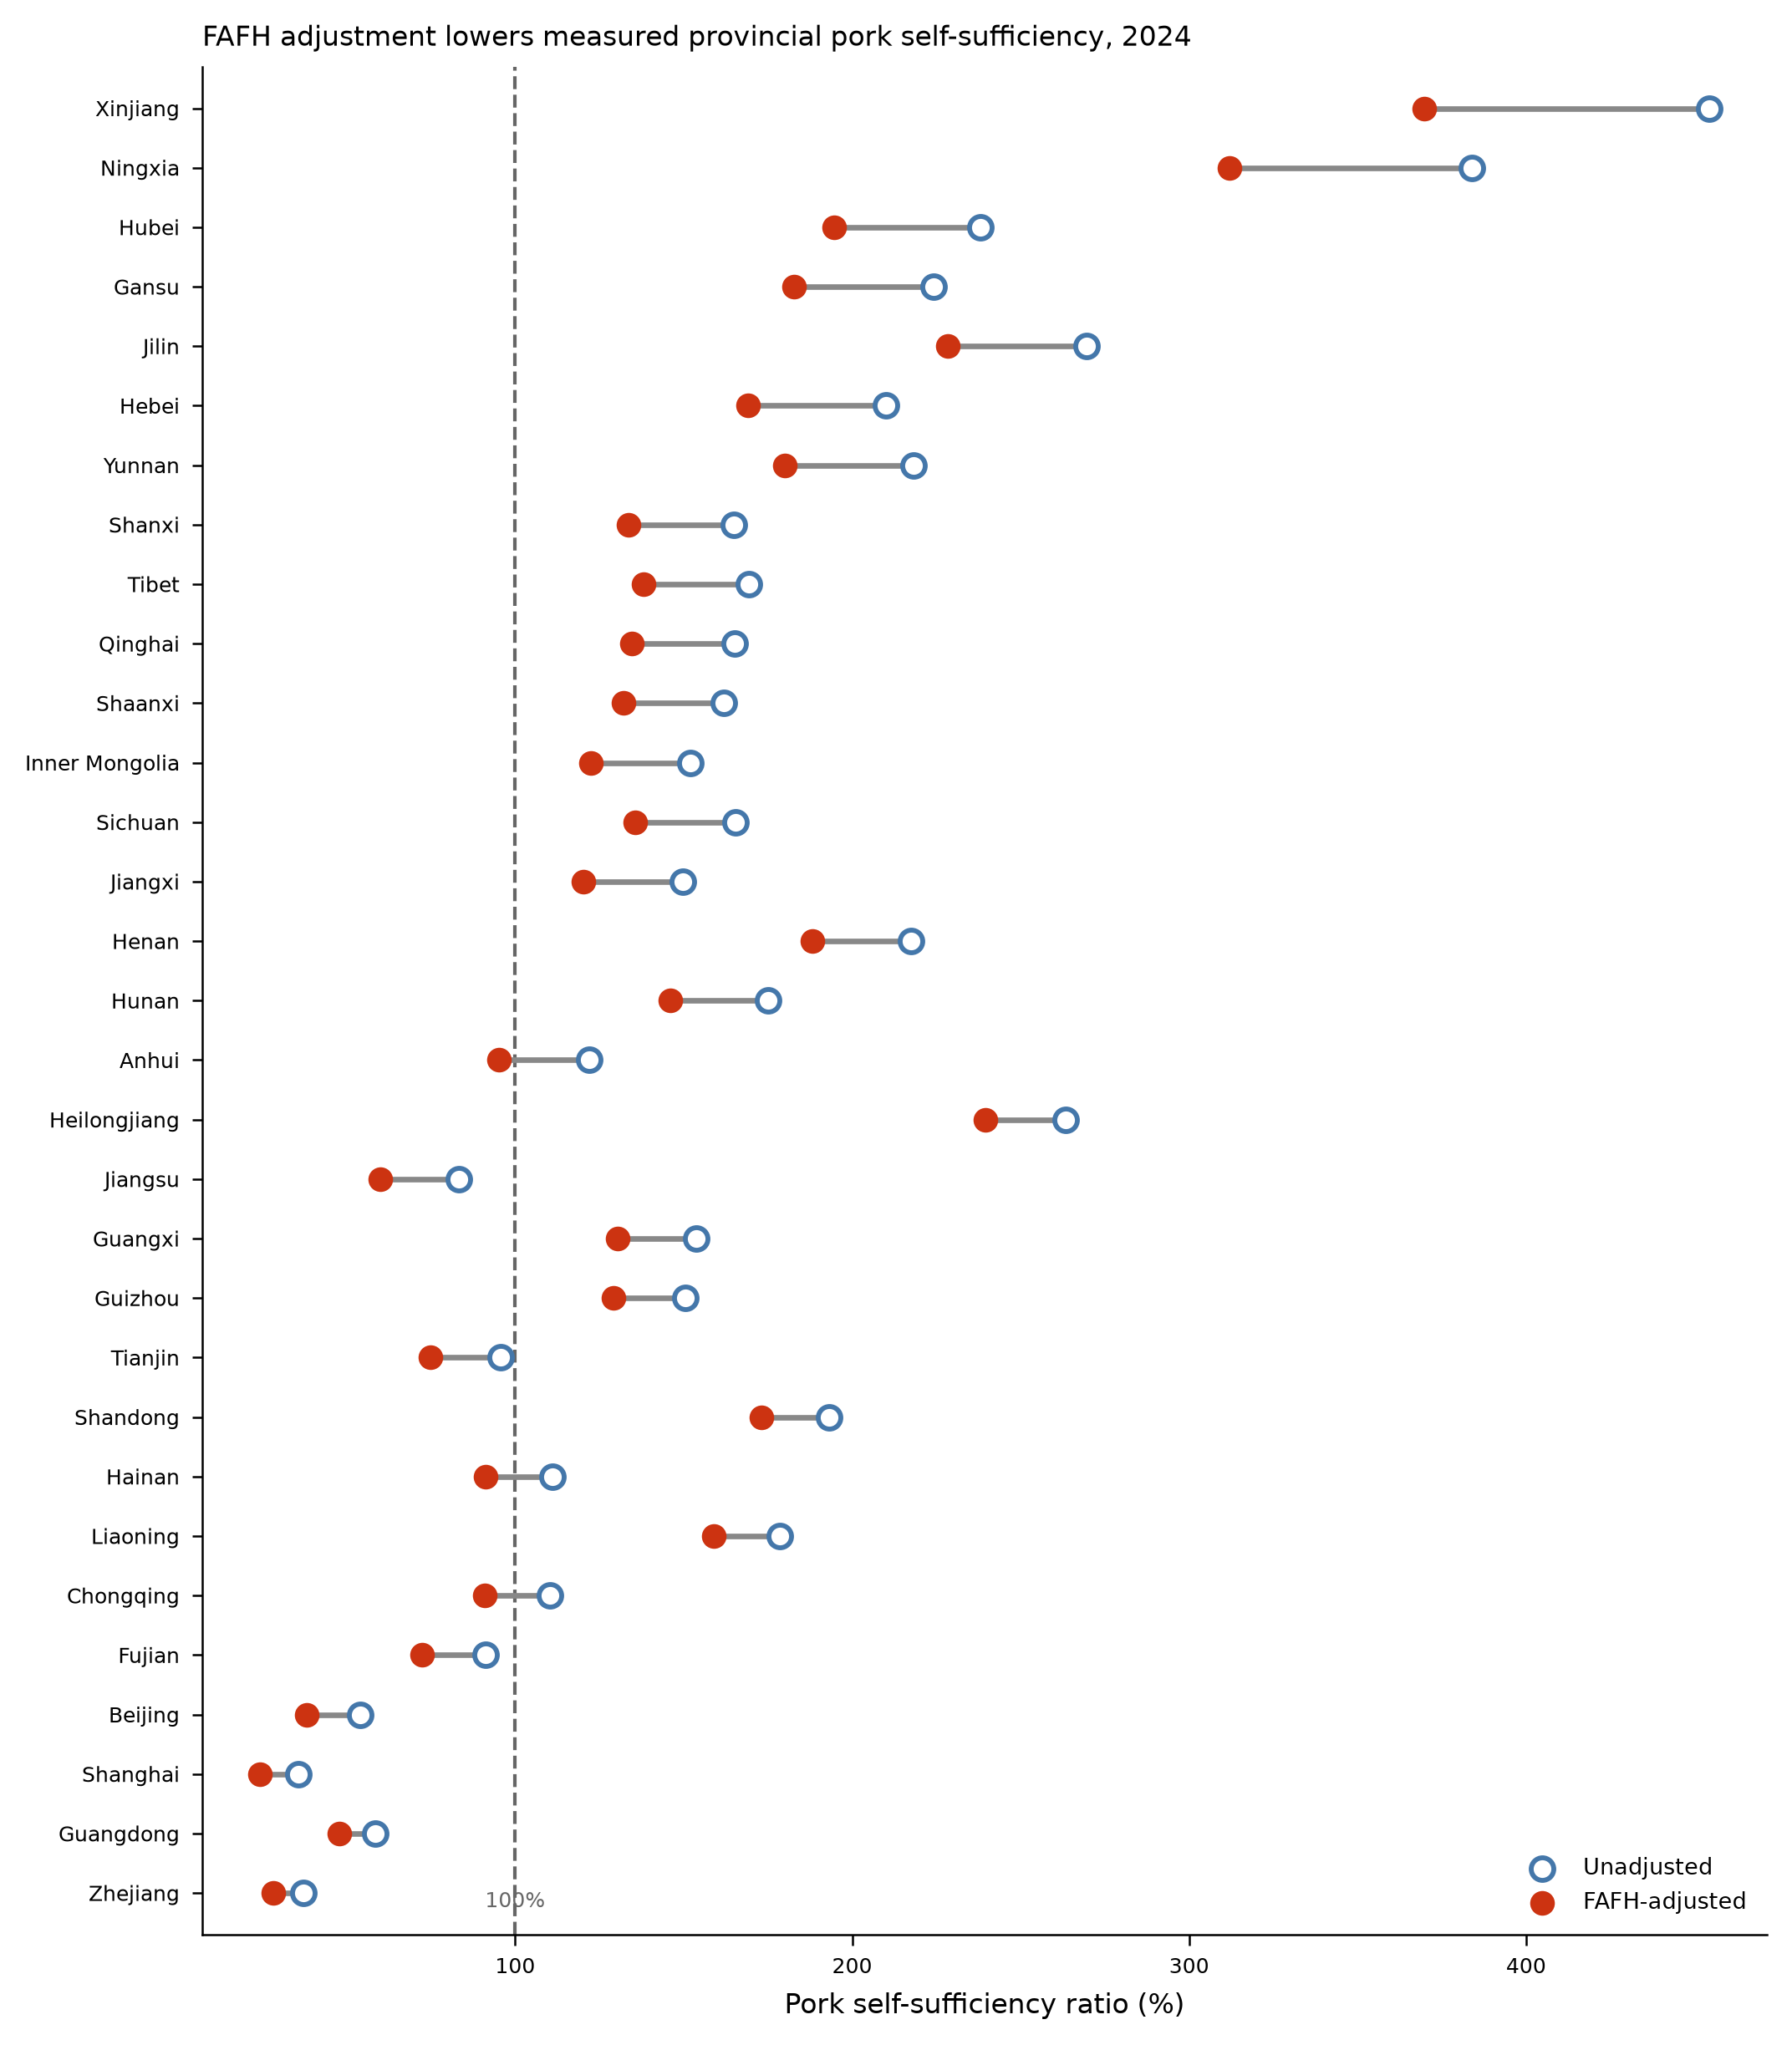
\includegraphics[width=0.95\linewidth]{fig6_ssr_dumbbell.png}}{\fbox{\parbox{0.9\linewidth}{\centering\vspace{2em}Figure~6: provincial pork self-sufficiency ratios, unadjusted vs.\ adjusted, 2024 (dumbbell chart)\vspace{2em}}}}
\caption{Provincial pork self-sufficiency ratios with and without FAFH adjustment, 2024. Each dumbbell connects the unadjusted ratio (hollow marker) to the adjusted ratio (solid marker); provinces are ordered by the size of the decline. The dashed vertical line marks self-sufficiency of 100 percent.}
\label{fig:ssr_dumbbell}
\end{figure}

Three caveats bound these exercises. First, they are accounting translations, not counterfactual equilibria: consumption, production, and trade do not respond to the correction within the calculation. Second, the conversion coefficients---edible portions, energy and protein contents, and feed-conversion ratios---are standard published values with their own uncertainty, which the bootstrap intervals do not capture; the retail-weight factors used to place carcass-weight production on a survey-comparable basis (Appendix Table~\ref{tab:coefficients}) are a modeling choice rather than a sourced coefficient. Applying the lower nominal food-balance factors (pork 0.78, beef 0.72, poultry 0.88) instead would shrink supply-side availability, narrow the supply--survey gap, and thereby inflate the closure shares to implausible levels (above 100 percent for pork); the survey-comparable factors are the conservative choice for this reason. Third, the indicators inherit the extrapolation caveats of Section~\ref{sec:validation}, and the model-choice sensitivity reported in Appendix Table~\ref{tab:app_sensitivity} shows that the qualitative conclusions---the over-ceiling classification and understated severity for livestock meat, substantial gap closure for pork, and material self-sufficiency declines for animal-source foods---hold under the LightGBM and Random Forest factors, although magnitudes vary. Within those bounds, the answer to the section's question is unambiguous: the measurement error is not a technical detail; it is large enough to change what China's food statistics say about nutrition adequacy, statistical consistency, and self-sufficiency.

% =====================================================================
\section{Discussion}
\label{sec:discussion}

\subsection{What the adjustment factors add to the literature}

The results address a measurement gap identified but not resolved by previous research. The ``missing meat'' and survey-account discrepancy literature shows that FAH survey quantities cannot fully reconcile with supply-side food accounts in China \citep{MaHuangRozelle2004, YuAbler2014, Xiao2015, YuAbler2016}. The FAFH behavior literature explains why this gap has grown: rising incomes, urbanization, time constraints, canteen meals, restaurant use, and delivery platforms all increase the share of meals obtained outside the home \citep{Ma2006, Bai2010, Bai2012, Liu2015, GaoZheng2020}. This paper links those two strands twice over. It provides a practical set of physical-quantity multipliers that can be applied to FAH data, and it uses those multipliers to place numbers on the policy stakes: the correction accounts for roughly 69 percent of the pork supply--consumption gap, sharpens the dietary-guideline assessment for livestock and poultry meat from an apparent to a substantially larger exceedance of the ceiling, and lowers measured animal-source self-sufficiency by 4--36 percentage points (Section~\ref{sec:applications}).

The commodity pattern is consistent with the literature and with food-service practice. Larger corrections for poultry, beef, pork, and aquatic products reflect the importance of animal-source foods in restaurants, canteens, and prepared meals. Smaller corrections for dairy, eggs, and fruits are consistent with more household-centered consumption. The implication is that FAFH omission does not simply shift the level of demand downward; it also changes the apparent structure of the diet. This is precisely the type of compositional bias that survey-measurement studies warn about when FAFH is captured only in expenditure or omitted from physical quantities \citep{Zezza2017, FiedlerYadav2017, ReitzigEtAl2023}.

The spatial pattern also extends existing work. Earlier Chinese FAFH studies document strong income and urban effects in particular cities or samples \citep{Bai2010, Liu2015}. The estimates here translate that behavioral gradient into province-level demand corrections. Metropolitan and coastal provinces require larger multipliers than inland and more agricultural provinces. This finding is important for food-policy analysis because provincial food balances and self-sufficiency assessments are sensitive not only to total demand but also to where demand is located.

\subsection{Implications for food policy and statistics}

The most direct users of the adjustment factors are analysts and agencies that rely on FAH quantity data but lack commodity-specific FAFH quantities, and the applications in Section~\ref{sec:applications} indicate what is at stake for each. For statistical agencies, the factors reconcile a quantified share of the household--balance-sheet wedge, so the residual that genuinely requires investigation is 31 percent of the raw pork gap rather than all of it. For nutrition monitoring under the Healthy China agenda, guideline comparisons based on at-home quantities understate the food groups that matter most: livestock-meat intake, already above the guideline ceiling in at-home data, is revealed to stand 115 percent above it once FAFH is counted, while the dairy shortfall survives adjustment and therefore warrants demand-side policy rather than statistical repair. For food-security planning, adjusted demand lowers measured animal-source self-sufficiency by 4--36 percentage points nationally and by up to 84.4 points in individual producing provinces, and adds 61.6 million tonnes to implied feed-grain requirements---magnitudes that belong in baseline projections, not in footnotes. Researchers estimating demand systems from secondary household quantity data can use the factors as a transparent correction when direct FAFH quantities are unavailable.

The policy implication is not that model-based factors should replace direct measurement. The preferred long-term solution is improved survey design: household surveys should periodically collect source-specific food quantities, or dietary recall modules should be harmonized with acquisition modules so that FAH and FAFH can be separated by commodity. Until that is routine, adjustment factors provide an interim bridge between existing data systems and the way food is actually consumed. Their value is greatest in contexts where (i) FAH quantities are observed, (ii) FAFH quantities are missing or only observed as aggregate expenditure, and (iii) external covariates or benchmarks are available to support projection and validation.

For food-balance reconciliation, the results imply that apparent self-sufficiency can be overstated when FAH quantities are used as the demand denominator. This point is most salient for animal-source foods and for provinces with dense food-service markets. For nutrition and dietary monitoring, the results imply that quantity-based studies relying only on home foods may understate the role of animal-source and prepared foods in urban diets. Adjustment factors do not measure diet quality, but they help align quantity measurement with contemporary consumption channels.

\subsection{Scope and limitations}
\label{subsec:limits}

The framework is predictive rather than causal. It estimates a measurement correction, not the causal effect of income, urbanization, or food-service development on FAFH behavior. Researchers interested in mechanisms should use designs that address endogeneity directly and treat these factors as measurement inputs rather than causal estimates.

Temporal extrapolation is the main limitation. The micro relationship is learned from CHNS waves through 2011 and projected to 2015--2024. Macro covariates capture part of the subsequent change in income, urbanization, and food-service development, but they cannot fully measure platform-based delivery, prepared-food retailing, macroeconomic turbulence during the COVID-19 period, recessionary pressures, or international trade conflicts. The drop-last-wave diagnostic is reassuring within the CHNS period, but it is not a substitute for newer microdata.

Spatial extrapolation is a second limitation. Several provinces are not directly represented in the CHNS estimation sample, and Beijing and Shanghai are observed only in 2011. The leave-one-province-out diagnostic suggests that core provinces can be predicted reasonably well, but it also shows larger errors when a province occupies a distinctive position in the covariate distribution. Users should therefore avoid treating the factors as precise subprovincial estimates and should pay particular attention to uncertainty when applying them to provinces with food-service structures far from the CHNS support.

A third caveat concerns the application layer. The indicators in Section~\ref{sec:applications} depend on published conversion coefficients and on food-balance components measured with their own error; the bootstrap intervals propagate uncertainty in the adjustment factors but not in those inputs. The exercises should therefore be read as bounding the policy relevance of the FAFH correction under standard accounting conventions, not as revised official statistics.

Category coverage is a further limitation. Edible oil, mutton, and sugar are excluded from headline reporting because their source-specific support is thin or unreliable. This choice avoids spurious precision, but it also marks a boundary of the evidence. Future survey rounds could address this by recording bulk-purchased foods, condiments, oils, and regionally concentrated foods in a way that preserves source information over the recall period. Doing so would make a more comprehensive food-balance correction possible.

These limitations do not overturn the central conclusion. Across specifications, categories, and diagnostics, the adjustment factors exceed one and are larger for foods and provinces where FAFH is expected to matter most. The appropriate interpretation is therefore cautious but useful: the factors are not definitive consumption statistics, but they are more informative than assuming that FAH quantities equal total consumption.

% =====================================================================
\section{Conclusion and policy implications}
\label{sec:conclusion}

Food away from home is no longer a residual component of food consumption in China. It is central to how households obtain meals and therefore to how food demand should be measured. This paper estimates province-year and commodity-specific adjustment factors that convert FAH quantities into total consumption. The framework predicts a bounded at-home ratio, converts it into an interpretable reciprocal multiplier, and evaluates the resulting projections through model benchmarks, bootstrap intervals, external expenditure checks, spatial diagnostics, and temporal stability tests.

The main conclusion is that FAH data systematically understate total consumption, that the understatement is not uniform, and that it is large enough to change policy assessments. The correction is larger for animal-source foods and for more urbanized provinces. Counting FAFH sharpens the dietary-guideline assessment for livestock and poultry meat, revealing intake at 115 percent above the recommended ceiling rather than the smaller exceedance seen in at-home data, while confirming that the dairy shortfall is real; it closes roughly 69 percent of the documented pork supply--consumption gap; and it lowers measured self-sufficiency for major animal-source foods by 4--36 percentage points while adding 61.6 million tonnes to implied feed-grain requirements. Ignoring FAFH therefore biases the level, composition, and geography of measured demand---and with them the nutrition and food-security conclusions built on household statistics.

The adjustment factors are most applicable to studies and agencies using secondary food-at-home quantity data that lack commodity-specific FAFH information. National factors may be useful for broad aggregate exercises, but provincial planning requires province-specific factors. The next step is direct measurement: future CHNS waves or comparable national surveys should collect commodity-specific FAFH quantities, including difficult categories such as edible oil, sugar, condiments, and regionally concentrated meats. Until those data become routine, transparent and validated adjustment factors provide a practical bridge between existing statistical systems and contemporary consumption behavior.

\section*{CRediT authorship contribution statement}
Author contributions are omitted from the anonymized manuscript and will be supplied in the submission system.

\section*{Declaration of competing interests}
The authors declare that they have no known competing financial interests or personal relationships that could have appeared to influence the work reported in this paper.

\section*{Data availability}
The China Health and Nutrition Survey data are available from the Carolina Population Center under a user agreement. All other inputs are published official statistics. Replication code, intermediate data files, the province-year adjustment-factor series with bootstrap replicates, the category-mapping table, and the worksheets underlying the food-security and nutrition applications in Section~\ref{sec:applications} are available from the corresponding author upon reasonable request.

\bibliographystyle{elsarticle-harv}
\bibliography{reference-FP}

\newpage
% =====================================================================
\appendix
\setcounter{table}{0}
\setcounter{figure}{0}
\renewcommand{\thetable}{A.\arabic{table}}
\renewcommand{\thefigure}{A.\arabic{figure}}
\renewcommand{\theHtable}{A.\arabic{table}}
\renewcommand{\theHfigure}{A.\arabic{figure}}

\section{Supplementary tables and figures}
\label{app:supplementary}

\begin{table}[htbp]
\centering
\begin{threeparttable}
\caption{Best-performing model by food category in the bounded benchmark}
\label{tab:best_by_cat}
\small
\setlength{\tabcolsep}{0pt}
\begin{tabular*}{\textwidth}{@{\extracolsep{\fill}} lcc @{}}
\toprule
Food category & Best model & AF MAE \\
\midrule
Rice             & FT-Transformer & 0.219 \\
Wheat            & FT-Transformer & 0.432 \\
Legumes          & FT-Transformer & 0.304 \\
Coarse grains    & FT-Transformer & 0.423 \\
Vegetables       & FT-Transformer & 0.170 \\
Fruits           & FT-Transformer & 0.101 \\
Pork             & FT-Transformer & 0.253 \\
Beef             & FT-Transformer & 0.158 \\
Poultry          & FT-Transformer & 0.132 \\
Aquatic products & FT-Transformer & 0.224 \\
Eggs             & FT-Transformer & 0.143 \\
Dairy            & FT-Transformer & 0.103 \\
\bottomrule
\end{tabular*}
\begin{tablenotes}[flushleft]
\scriptsize
\item Notes: Results are based on the unified bounded benchmark. AF = adjustment factor; MAE = mean absolute error. FT-Transformer is the best-performing model for each of the twelve headline categories in this benchmark.
\end{tablenotes}
\end{threeparttable}
\end{table}

\begin{table}[htbp]
\centering
\begin{threeparttable}
\caption{Full province-level 2024 adjustment factors for selected categories}
\label{tab:prov2024_full}
\small
\setlength{\tabcolsep}{0pt}
\begin{tabular*}{\textwidth}{@{\extracolsep{\fill}} l cccc @{}}
\toprule
Province & Rice & Vegetables & Pork & Aquatic products \\
\midrule
Beijing       & 1.500 & 1.344 & 1.451 & 1.515 \\
Tianjin       & 1.344 & 1.194 & 1.314 & 1.345 \\
Hebei         & 1.294 & 1.169 & 1.274 & 1.292 \\
Shanxi        & 1.283 & 1.164 & 1.265 & 1.280 \\
Inner Mongolia & 1.297 & 1.171 & 1.279 & 1.295 \\
Liaoning      & 1.193 & 1.161 & 1.183 & 1.195 \\
Jilin         & 1.205 & 1.171 & 1.196 & 1.210 \\
Heilongjiang  & 1.197 & 1.169 & 1.187 & 1.201 \\
Shanghai      & 1.533 & 1.377 & 1.492 & 1.528 \\
Jiangsu       & 1.235 & 1.135 & 1.257 & 1.245 \\
Zhejiang      & 1.371 & 1.275 & 1.364 & 1.348 \\
Anhui         & 1.278 & 1.161 & 1.277 & 1.278 \\
Fujian        & 1.358 & 1.266 & 1.351 & 1.338 \\
Jiangxi       & 1.316 & 1.218 & 1.320 & 1.307 \\
Shandong      & 1.251 & 1.142 & 1.270 & 1.255 \\
Henan         & 1.163 & 1.117 & 1.204 & 1.189 \\
Hubei         & 1.184 & 1.127 & 1.222 & 1.214 \\
Hunan         & 1.175 & 1.120 & 1.214 & 1.207 \\
Guangdong     & 1.330 & 1.245 & 1.327 & 1.318 \\
Guangxi       & 1.230 & 1.150 & 1.213 & 1.224 \\
Hainan        & 1.337 & 1.253 & 1.332 & 1.323 \\
Chongqing     & 1.301 & 1.185 & 1.269 & 1.294 \\
Sichuan       & 1.241 & 1.144 & 1.224 & 1.249 \\
Guizhou       & 1.205 & 1.126 & 1.184 & 1.329 \\
Yunnan        & 1.199 & 1.128 & 1.200 & 1.247 \\
Tibet         & 1.273 & 1.169 & 1.245 & 1.284 \\
Shaanxi       & 1.235 & 1.147 & 1.218 & 1.238 \\
Gansu         & 1.224 & 1.142 & 1.205 & 1.221 \\
Qinghai       & 1.287 & 1.165 & 1.223 & 1.275 \\
Ningxia       & 1.246 & 1.152 & 1.223 & 1.242 \\
Xinjiang      & 1.216 & 1.139 & 1.208 & 1.217 \\
\bottomrule
\end{tabular*}
\begin{tablenotes}[flushleft]
\scriptsize
\item Notes: The four displayed categories are used in the main provincial analysis because they represent a staple (rice), a plant-food category (vegetables), a major meat category (pork), and aquatic products. Values are FT-Transformer point estimates for 2024. Full category-by-province estimates are available in the replication files.
\end{tablenotes}
\end{threeparttable}
\end{table}

\begin{table}[htbp]
\centering
\begin{threeparttable}
\caption{Summary of 2024 uncertainty: bootstrap confidence-interval widths}
\label{tab:uncertainty}
\small
\setlength{\tabcolsep}{0pt} 
\begin{tabular*}{\textwidth}{@{\extracolsep{\fill}} l cccc @{}}
\toprule
Food category & \shortstack{2024\\estimate} & \shortstack{National\\CI width} & \shortstack{Relative\\width} & \shortstack{Mean provincial\\CI width} \\
\midrule
Rice             & 1.276 & 0.345 & 27.07\% & 0.357 \\
Wheat            & 1.261 & 0.196 & 15.57\% & 0.194 \\
Legumes          & 1.261 & 0.240 & 19.00\% & 0.243 \\
Coarse grains    & 1.206 & 0.207 & 17.14\% & 0.207 \\
Vegetables       & 1.204 & 0.226 & 18.73\% & 0.233 \\
Fruits           & 1.117 & 0.159 & 14.23\% & 0.161 \\
Pork             & 1.273 & 0.300 & 23.58\% & 0.305 \\
Beef             & 1.363 & 0.320 & 23.49\% & 0.318 \\
Poultry          & 1.405 & 0.438 & 31.19\% & 0.456 \\
Aquatic products & 1.267 & 0.385 & 30.37\% & 0.410 \\
Eggs             & 1.126 & 0.090 & 7.96\%  & 0.092 \\
Dairy            & 1.099 & 0.105 & 9.59\%  & 0.106 \\
\bottomrule
\end{tabular*}
\begin{tablenotes}[flushleft]
\scriptsize
\item Notes: CI = confidence interval. National CI width is the 97.5th percentile minus the 2.5th percentile of the bootstrap distribution for the national estimate. Relative width is national CI width divided by the 2024 estimate.
\end{tablenotes}
\end{threeparttable}
\end{table}

\begin{table}[htbp]
\centering
\begin{threeparttable}
\caption{Multiseed variance of the FT-Transformer AF MAE within food categories}
\label{tab:multiseed}
\small
\setlength{\tabcolsep}{0pt} 
\begin{tabular*}{\textwidth}{@{\extracolsep{\fill}} l cccc @{}}
\toprule
Food category & \shortstack{AF MAE\\(mean)} & \shortstack{AF MAE\\(SD)} & \shortstack{AF MAE\\(min)} & \shortstack{AF MAE\\(max)} \\
\midrule
Rice             & 0.377 & 0.0011 & 0.376 & 0.379 \\
Wheat            & 0.987 & 0.0020 & 0.984 & 0.989 \\
Legumes          & 0.384 & 0.0015 & 0.383 & 0.387 \\
Coarse grains    & 0.532 & 0.0012 & 0.530 & 0.534 \\
Vegetables       & 0.237 & 0.0012 & 0.236 & 0.239 \\
Pork             & 0.308 & 0.0014 & 0.306 & 0.310 \\
Beef             & 0.193 & 0.0021 & 0.191 & 0.195 \\
Poultry          & 0.177 & 0.0022 & 0.174 & 0.180 \\
Aquatic products & 0.286 & 0.0015 & 0.285 & 0.289 \\
Eggs             & 0.175 & 0.0006 & 0.175 & 0.176 \\
Dairy            & 0.125 & 0.0016 & 0.122 & 0.127 \\
Fruits           & 0.114 & 0.0005 & 0.113 & 0.115 \\
\midrule
\addlinespace
Across-category mean & 0.325 & 0.0014 & --- & --- \\
\bottomrule
\end{tabular*}
\begin{tablenotes}[flushleft]
\scriptsize
\item Notes: The FT-Transformer is trained under five seeds $\{1, 7, 42, 99, 123\}$ with the fixed-hyperparameter protocol. For each seed and category, fivefold cross-validation is run and AF MAE is averaged across folds. SD = across-seed standard deviation of this fold-averaged AF MAE. AF = adjustment factor; MAE = mean absolute error.
\end{tablenotes}
\end{threeparttable}
\end{table}

\begin{table}[htbp]
\centering
\begin{threeparttable}
\caption{Sensitivity of the unified bounded benchmark to the bounding parameter $\varepsilon$}
\label{tab:eps_sensitivity}
\small
\setlength{\tabcolsep}{0pt} 
\begin{tabular*}{\textwidth}{@{\extracolsep{\fill}} l ccccc @{}}
\toprule
Model & $\varepsilon=0.005$ & $\varepsilon=0.01$ & $\varepsilon=0.02$ & $\varepsilon=0.05$ & $\varepsilon=0.10$ \\
\midrule
FT-Transformer  & 0.266 & 0.252 & 0.238 & 0.227 & 0.247 \\
Tabular ResNet  & 0.277 & 0.261 & 0.247 & 0.232 & 0.249 \\
Lasso           & 0.293 & 0.277 & 0.263 & 0.247 & 0.255 \\
CatBoost        & 0.296 & 0.282 & 0.269 & 0.253 & 0.261 \\
LightGBM        & 0.297 & 0.283 & 0.271 & 0.256 & 0.264 \\
Random Forest   & 0.300 & 0.286 & 0.273 & 0.258 & 0.265 \\
XGBoost         & 0.316 & 0.302 & 0.290 & 0.277 & 0.285 \\
MLP             & 0.320 & 0.307 & 0.297 & 0.287 & 0.298 \\
Ridge           & 0.898 & 0.584 & 0.422 & 0.319 & 0.299 \\
\midrule
\addlinespace
Rank of top model (FT-Transformer) & 1 & 1 & 1 & 1 & 1 \\
Top-3 AF-MAE gap (3rd vs. 1st, \%) & 10.2 & 9.9 & 10.5 & 8.8 & 3.2 \\
\bottomrule
\end{tabular*}
\begin{tablenotes}[flushleft]
\scriptsize
\item Notes: Each cell reports adjustment-factor-scale mean absolute error (AF MAE), averaged across the twelve headline categories, after re-clipping saved out-of-sample predictions at the stated value of $\varepsilon$. No retraining is performed. XGBoost = Extreme Gradient Boosting; LightGBM = Light Gradient Boosting Machine; MLP = multilayer perceptron. The bounded design prevents a few near-zero predicted ratios from determining the model ranking, which makes the benchmark more informative for choosing a stable estimator for policy measurement.
\end{tablenotes}
\end{threeparttable}
\end{table}

\begin{table}[htbp]
\centering
\begin{threeparttable}
\caption{Cross-validation performance for the imputation stage}
\label{tab:imputation}
\small
\setlength{\tabcolsep}{0pt}
\begin{tabular*}{\textwidth}{@{\extracolsep{\fill}} l ccc @{}}
\toprule
Model & MAE & RMSE & Rank \\
\midrule
FT-Transformer & 0.157 & 0.267 & 1 \\
MLP            & 0.165 & 0.253 & 2 \\
TabM           & 0.167 & 0.254 & 3 \\
Random Forest  & 0.169 & 0.264 & 4 \\
CatBoost       & 0.170 & 0.263 & 5 \\
Ridge          & 0.171 & 0.267 & 6 \\
LightGBM       & 0.171 & 0.264 & 7 \\
Lasso          & 0.172 & 0.272 & 8 \\
XGBoost        & 0.180 & 0.279 & 9 \\
Tabular ResNet & 0.207 & 0.305 & 10 \\
TabNet         & 0.209 & 0.315 & 11 \\
\bottomrule
\end{tabular*}
\begin{tablenotes}[flushleft]
\scriptsize
\item Notes: Performance is evaluated through fivefold cross-validation on observed CHNS records. MAE = mean absolute error; RMSE = root mean squared error; MLP = multilayer perceptron; XGBoost = Extreme Gradient Boosting; LightGBM = Light Gradient Boosting Machine. The imputation model fills missing FAH/FAFH source splits before the primary adjustment-factor estimation.
\end{tablenotes}
\end{threeparttable}
\end{table}

\begin{table}[htbp]
\centering
\begin{threeparttable}
\caption{Coefficients used in the food-security and nutrition applications (Section~\ref{sec:applications})}
\label{tab:coefficients}
\small
\setlength{\tabcolsep}{0pt}
\begin{tabular*}{\textwidth}{@{\extracolsep{\fill}} l cccccc @{}}
\toprule
Commodity & \shortstack{Guideline\\group} & \shortstack{Edible\\portion} & \shortstack{Retail-weight\\factor} & \shortstack{Energy\\(kcal/100 g)} & \shortstack{Protein\\(g/100 g)} & \shortstack{Feed conversion\\(kg feed/kg product)} \\
\midrule
Rice             & Cereals          & 1.00 & --- & 346 & 7.9 & --- \\
Wheat            & Cereals          & 1.00 & --- & 344 & 12.4 & --- \\
Legumes          & Cereals          & 1.00 & --- & 329 & 20.0 & --- \\
Coarse grains    & Cereals          & 1.00 & --- & 348 & 8.5 & --- \\
Vegetables       & Vegetables       & 0.87 & --- & 31  & 1.9 & --- \\
Fruits           & Fruits           & 0.78 & --- & 52  & 0.5 & --- \\
Pork             & Livestock meat   & 1.00 & 0.95 & 331 & 15.1 & 2.8--3.2 \\
Beef             & Livestock meat   & 1.00 & 0.92 & 125 & 19.9 & 6.0--8.0 \\
Poultry          & Livestock meat   & 0.66 & 0.95 & 167 & 19.3 & 1.8--2.1 \\
Aquatic products & Aquatic products & 0.57 & 1.00 & 104 & 17.6 & 1.2--1.6 \\
Eggs             & Eggs             & 0.87 & 1.00 & 144 & 13.3 & 2.0--2.4 \\
Dairy            & Dairy            & 1.00 & 1.00 & 54  & 3.0  & 0.3--0.5 \\
\bottomrule
\end{tabular*}
\begin{tablenotes}[flushleft]
\scriptsize
\item Notes: Edible-portion, energy, and protein coefficients are consumption-weighted representative values from the China Food Composition Tables \citep{CFCT2019}; the mapping from CHNS items to representative foods is documented in the replication files. The retail-weight factor converts carcass-weight production to a basis comparable with the household survey for the reconciliation in Table~\ref{tab:reconciliation}. Because the NBS household quantities for meat are recorded as bone-in cuts close to carcass weight, rather than the trimmed boneless retail cut assumed by the nominal FAO food-balance factors \citep{FAO2001FBS}, we apply factors that net out only retail trim and loss (pork 0.95, beef 0.92, poultry 0.95) rather than the lower nominal factors. The lower nominal factors would shrink the supply--survey gap and inflate the closure shares (above 100 percent for pork), so the survey-comparable factors are the conservative choice; the sensitivity analysis in Appendix Table~\ref{tab:app_sensitivity} varies the adjustment-factor model and does not re-run the reconciliation under alternative retail-weight factors. Feed-conversion ratios are standard published values for Chinese production systems; sources are listed in the replication files.
\end{tablenotes}
\end{threeparttable}
\end{table}

\begin{table}[htbp]
\centering
\begin{threeparttable}
\caption{Sensitivity of the headline application indicators to the choice of prediction model}
\label{tab:app_sensitivity}
\small
\setlength{\tabcolsep}{0pt}
\begin{tabular*}{\textwidth}{@{\extracolsep{\fill}} l ccc @{}}
\toprule
Indicator & \shortstack{Baseline\\(FT-Transformer)} & LightGBM & \shortstack{Random\\Forest} \\
\midrule
Livestock-meat intake vs.\ guideline ceiling (\%)      & +115 & +101 & +113 \\
Dairy intake as share of guideline lower bound (\%)    & 13  & 12  & 12  \\
Pork supply--consumption gap closed (\%)               & 69  & 56  & 68  \\
Pork self-sufficiency change (pp)                      & $-$22.4 & $-$17.4 & $-$21.9 \\
Poultry self-sufficiency change (pp)                   & $-$35.7 & $-$18.2 & $-$15.3 \\
Additional feed-grain requirement (Mt)                 & 61.6 & 47.0 & 79.5  \\
\bottomrule
\end{tabular*}
\begin{tablenotes}[flushleft]
\scriptsize
\item Notes: Each column recomputes the Section~\ref{sec:applications} indicators using the national adjustment factors produced by the stated model (see Table~\ref{tab:robustness}), holding all accounting inputs fixed. The comparison separates model uncertainty from the bootstrap sampling uncertainty reported in the main tables.
\end{tablenotes}
\end{threeparttable}
\end{table}

\begin{figure}[htbp]
\centering
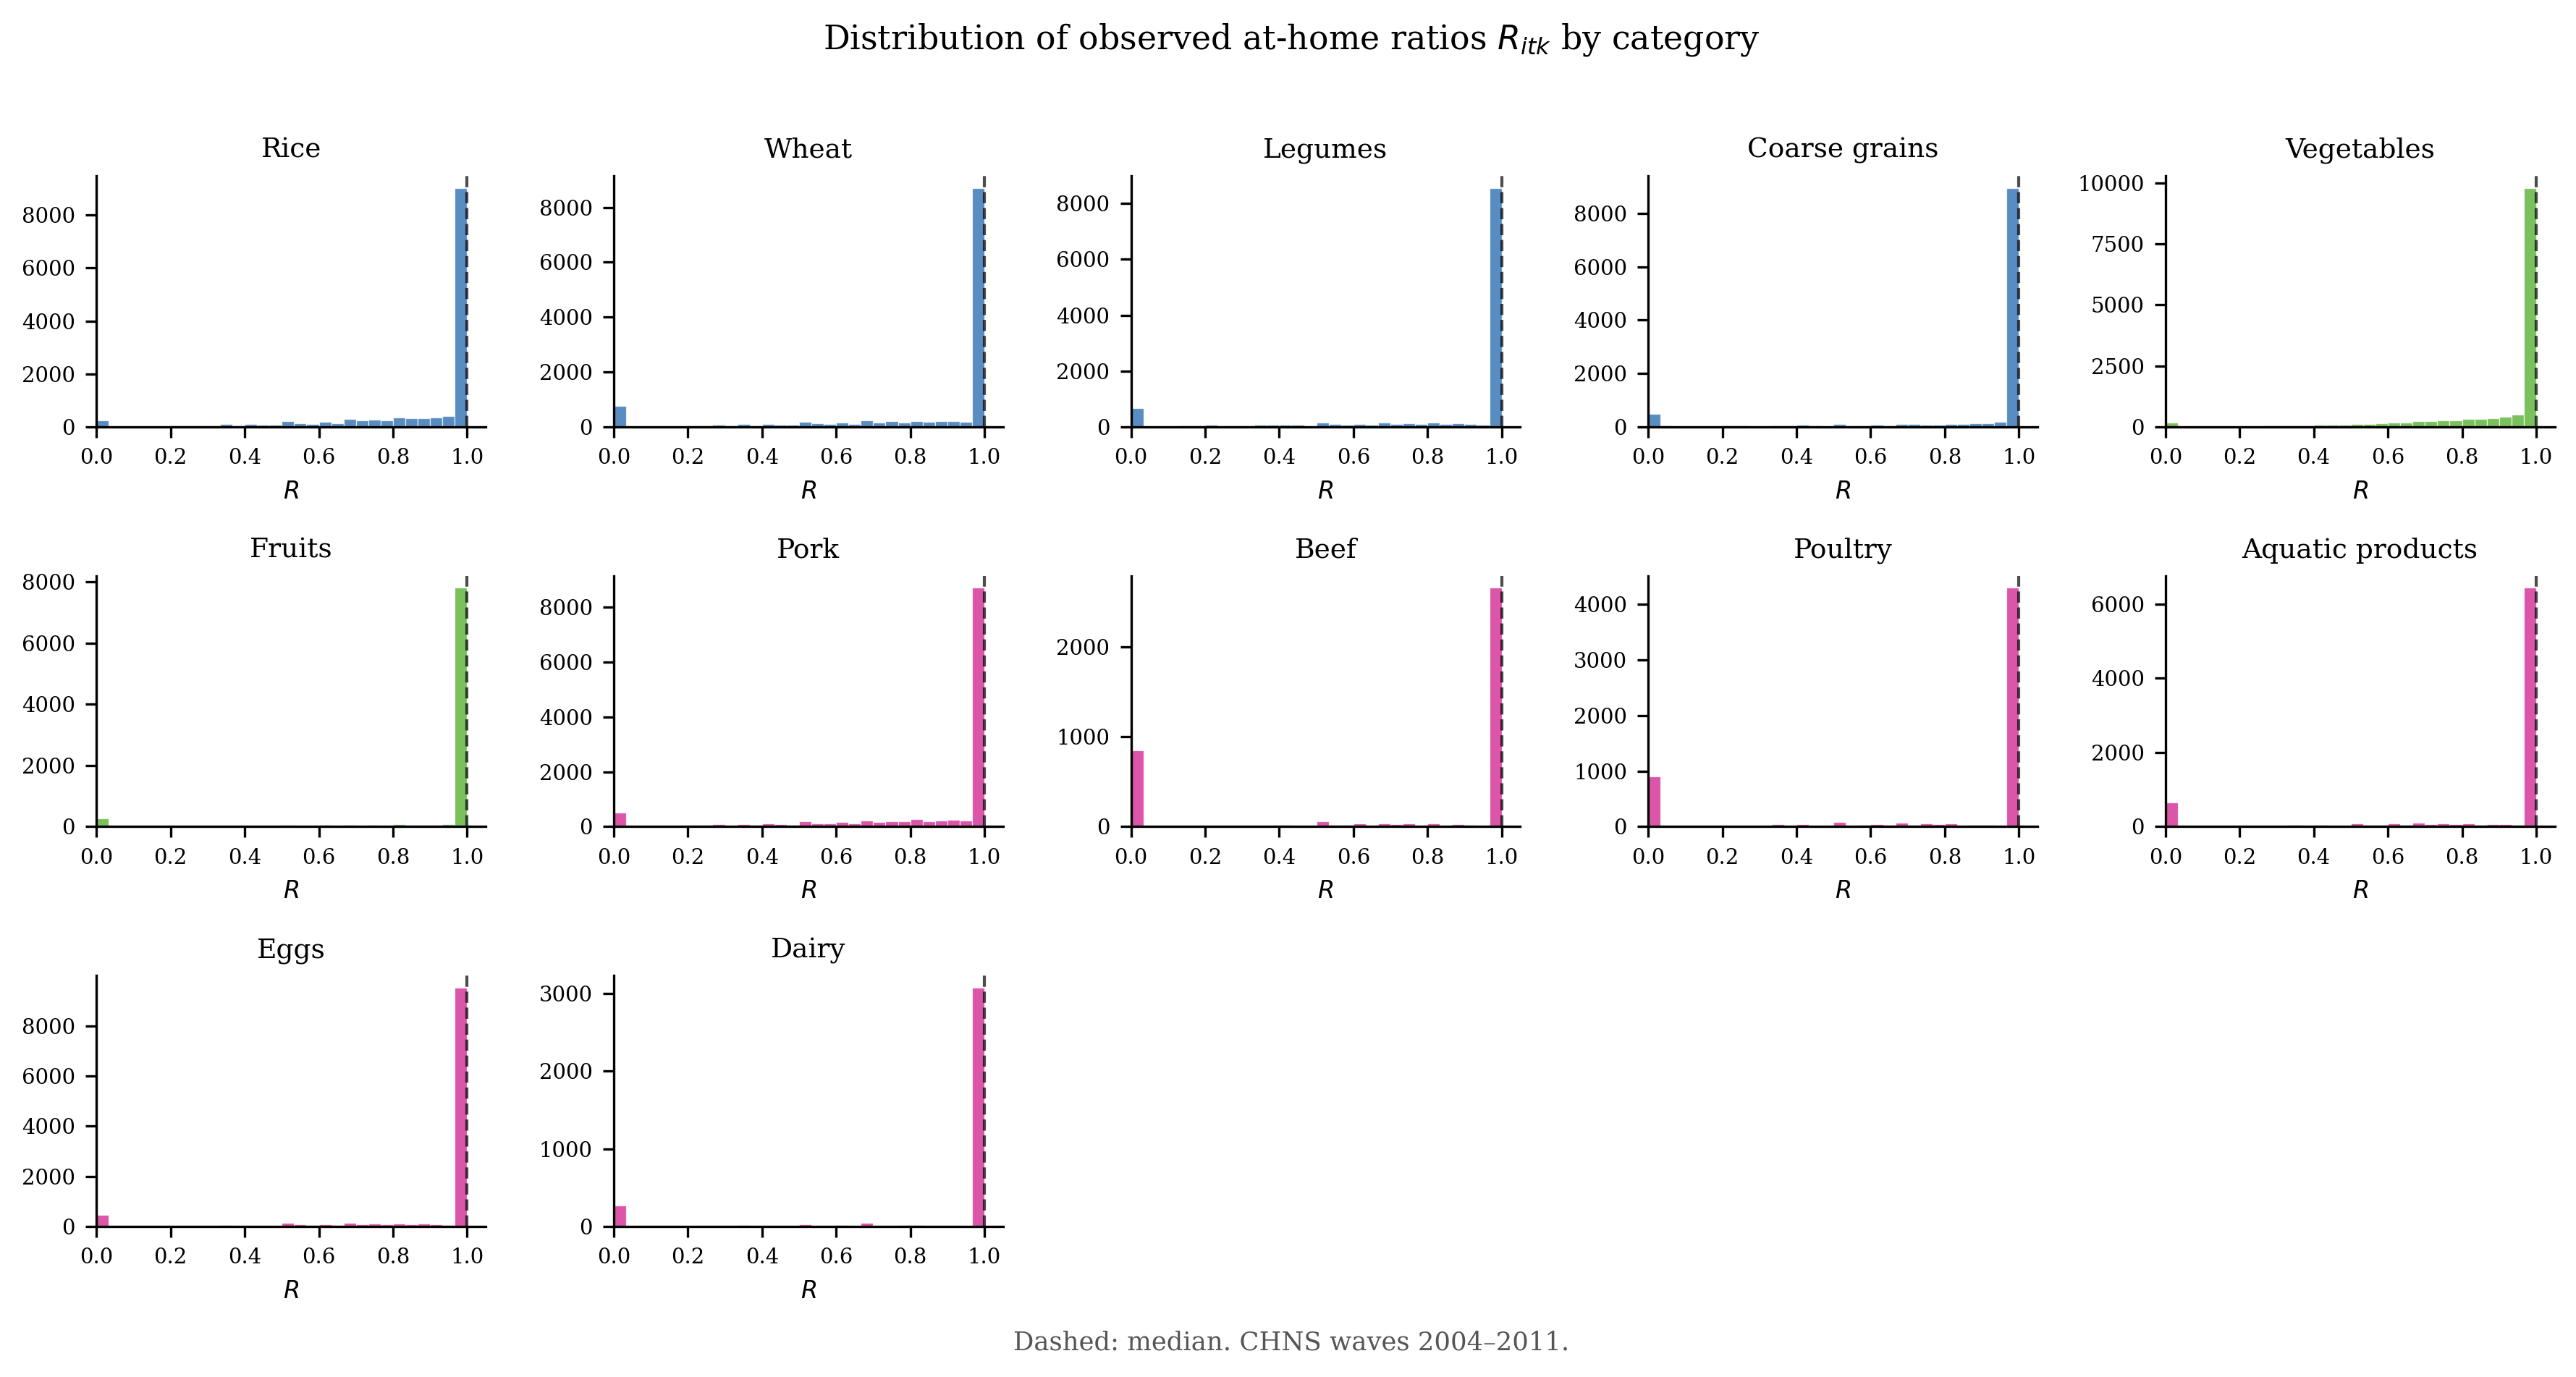
\includegraphics[width=1\linewidth]{figA1_ratio_distributions.png}
\caption{Distribution of observed household at-home ratios in the CHNS sample, by food category. Dashed vertical lines denote category medians.}
\label{fig:ratiohist}
\end{figure}

\begin{figure}[htbp]
\centering
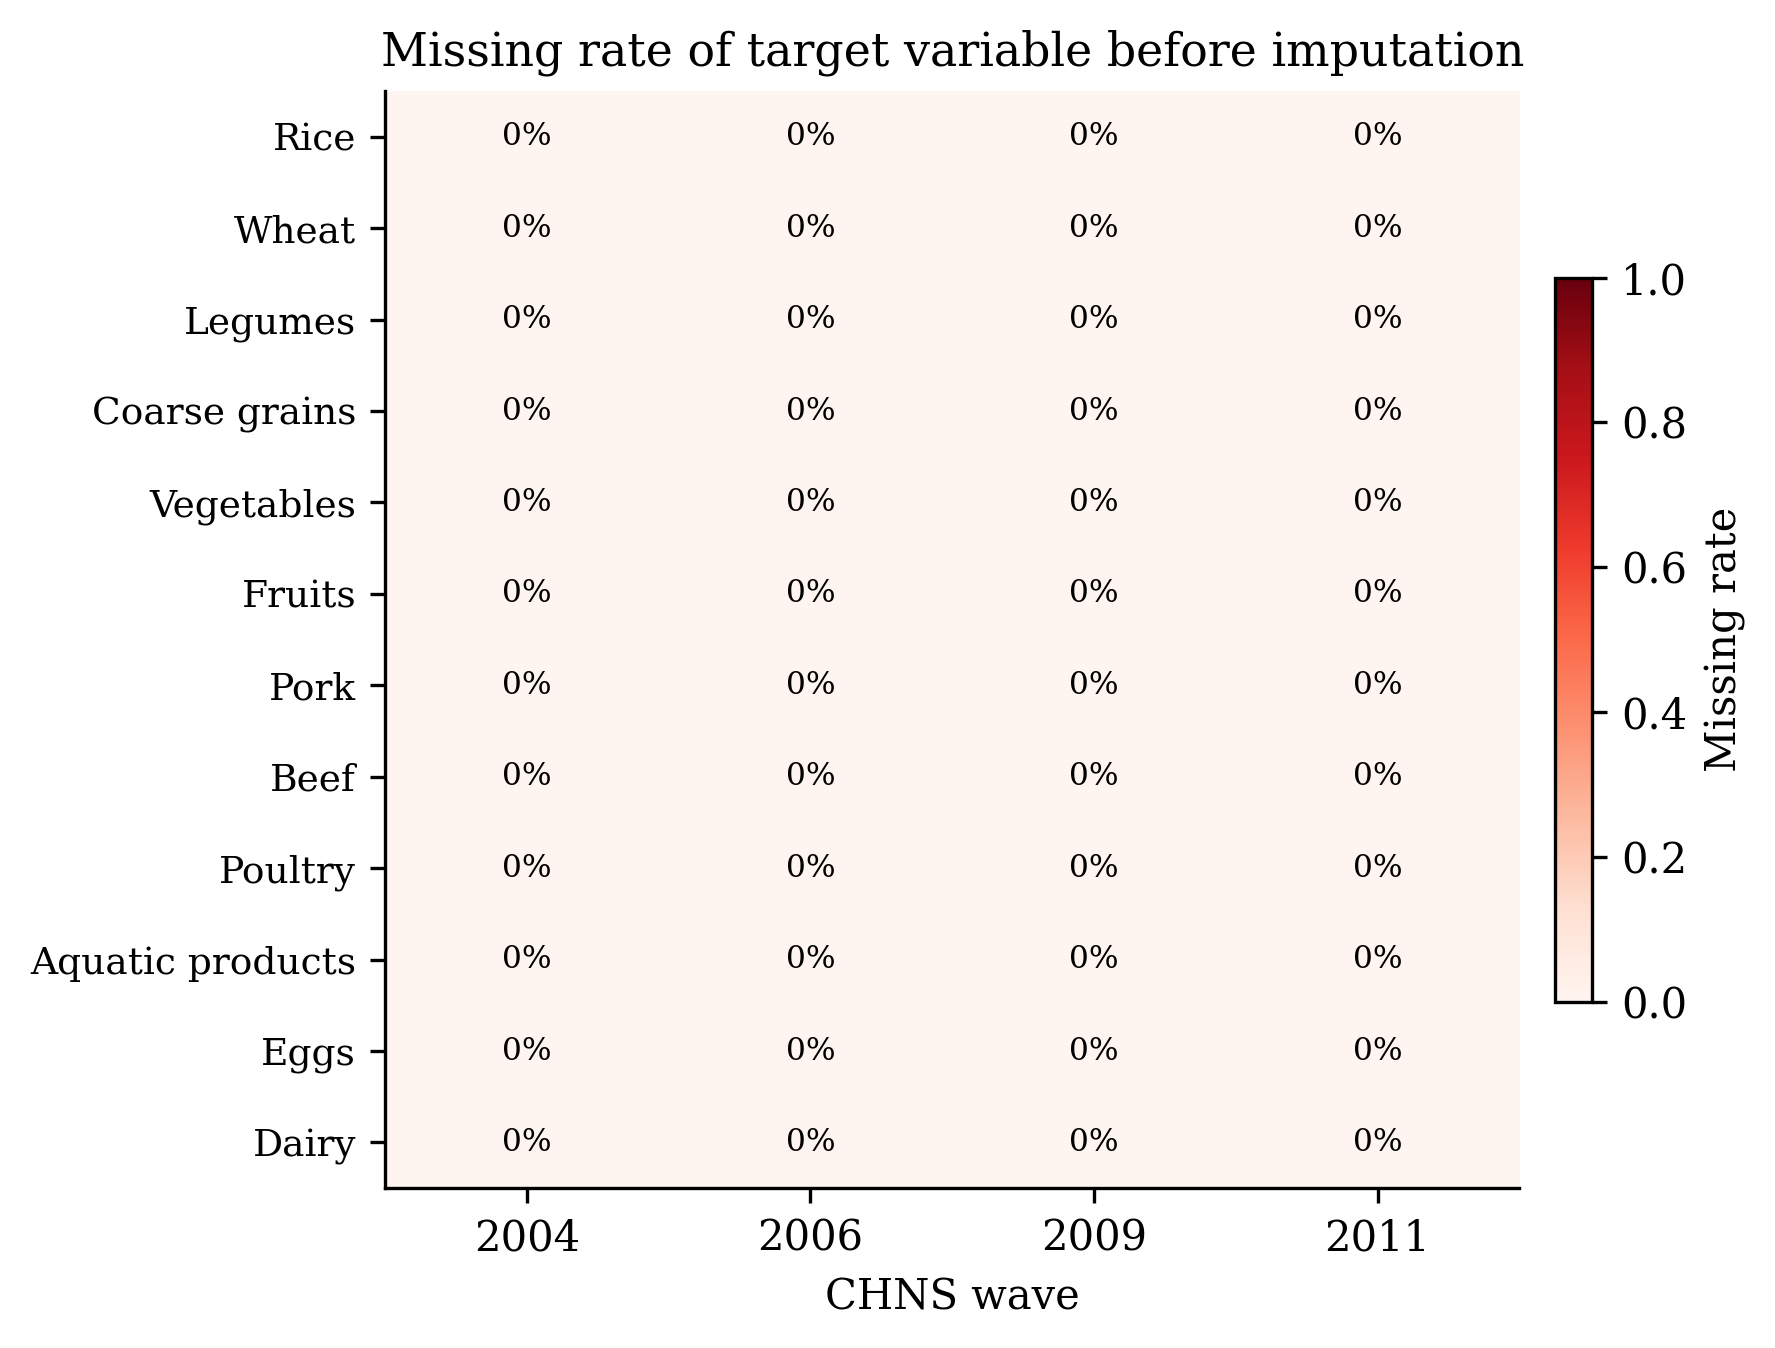
\includegraphics[width=0.78\linewidth]{figA2_missingness_heatmap.png}
\caption{Missing rate of the target variable before imputation, by CHNS wave and food category. CHNS = China Health and Nutrition Survey.}
\label{fig:missingness}
\end{figure}

\begin{figure}[htbp]
\centering
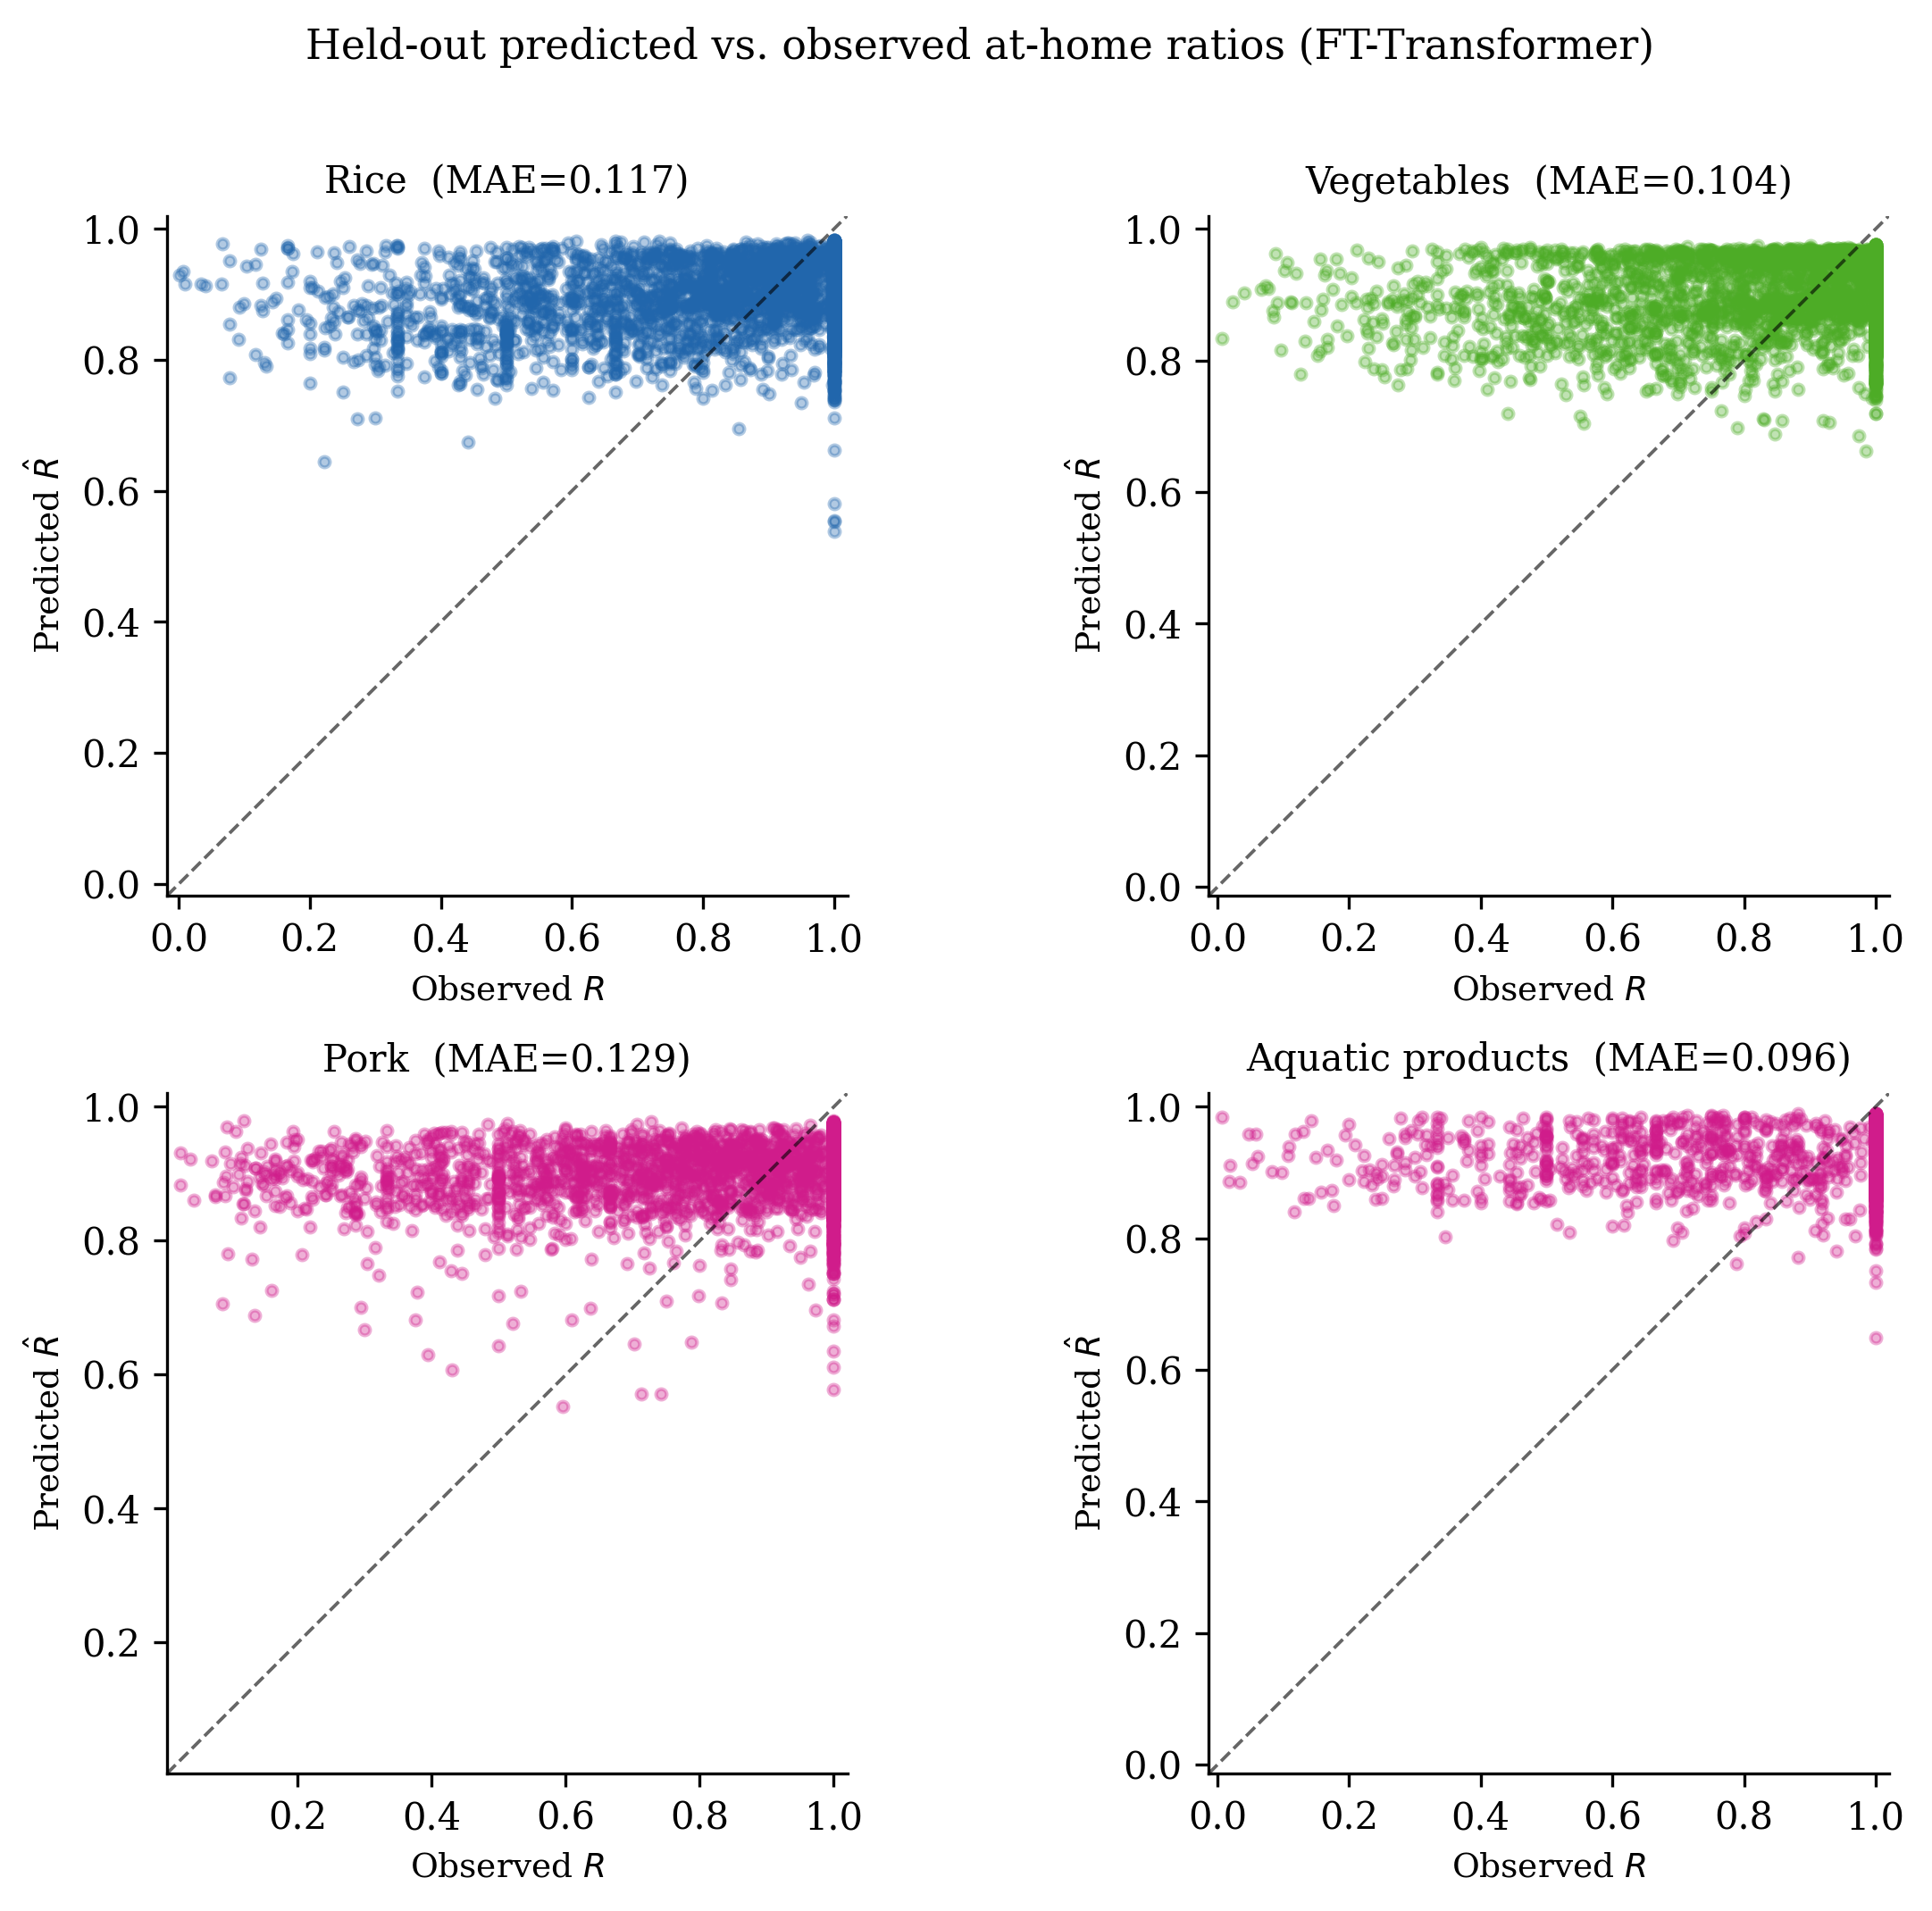
\includegraphics[width=1\linewidth]{figA3_pred_vs_obs.png}
\caption{Held-out predicted versus observed at-home ratios for the FT-Transformer in selected food categories. The dashed line is the 45-degree line.}
\label{fig:predobs}
\end{figure}

\begin{figure}[htbp]
\centering
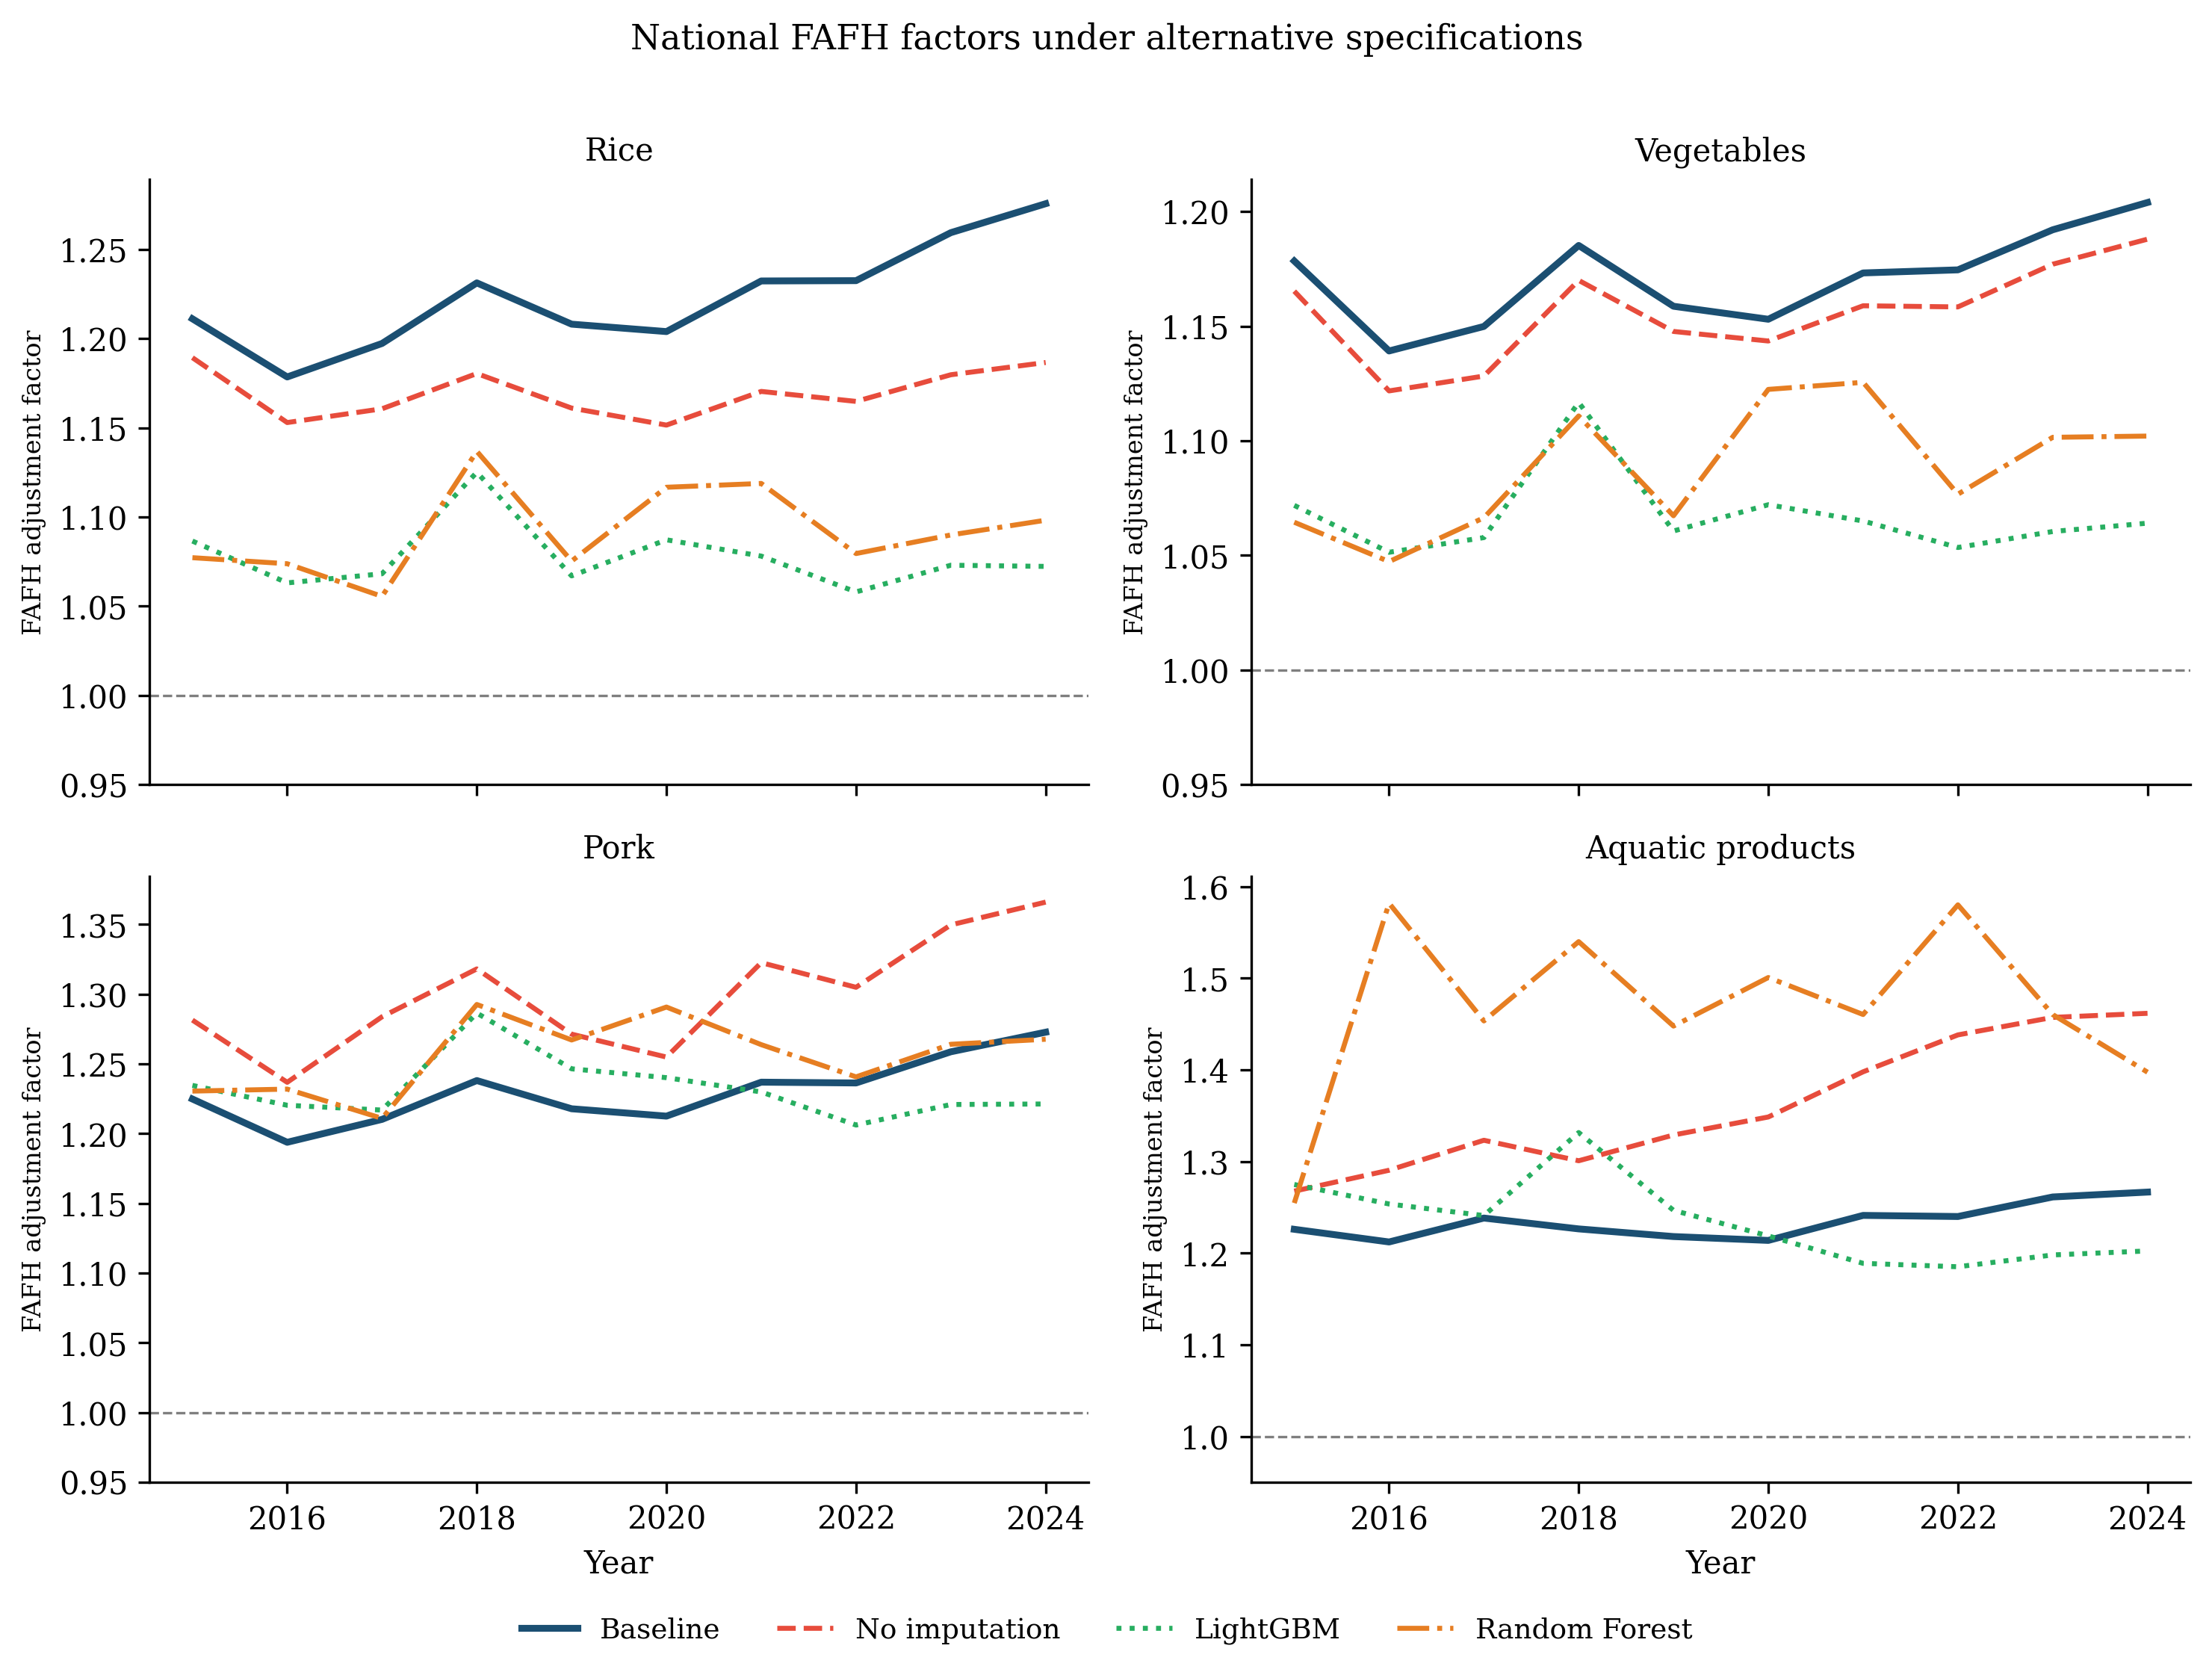
\includegraphics[width=1\linewidth]{figA5_alt_specs.png}
\caption{National food-away-from-home (FAFH) adjustment factors under alternative specifications for selected categories, 2015--2024.}
\label{fig:altspecs}
\end{figure}

\begin{figure}[htbp]
\centering
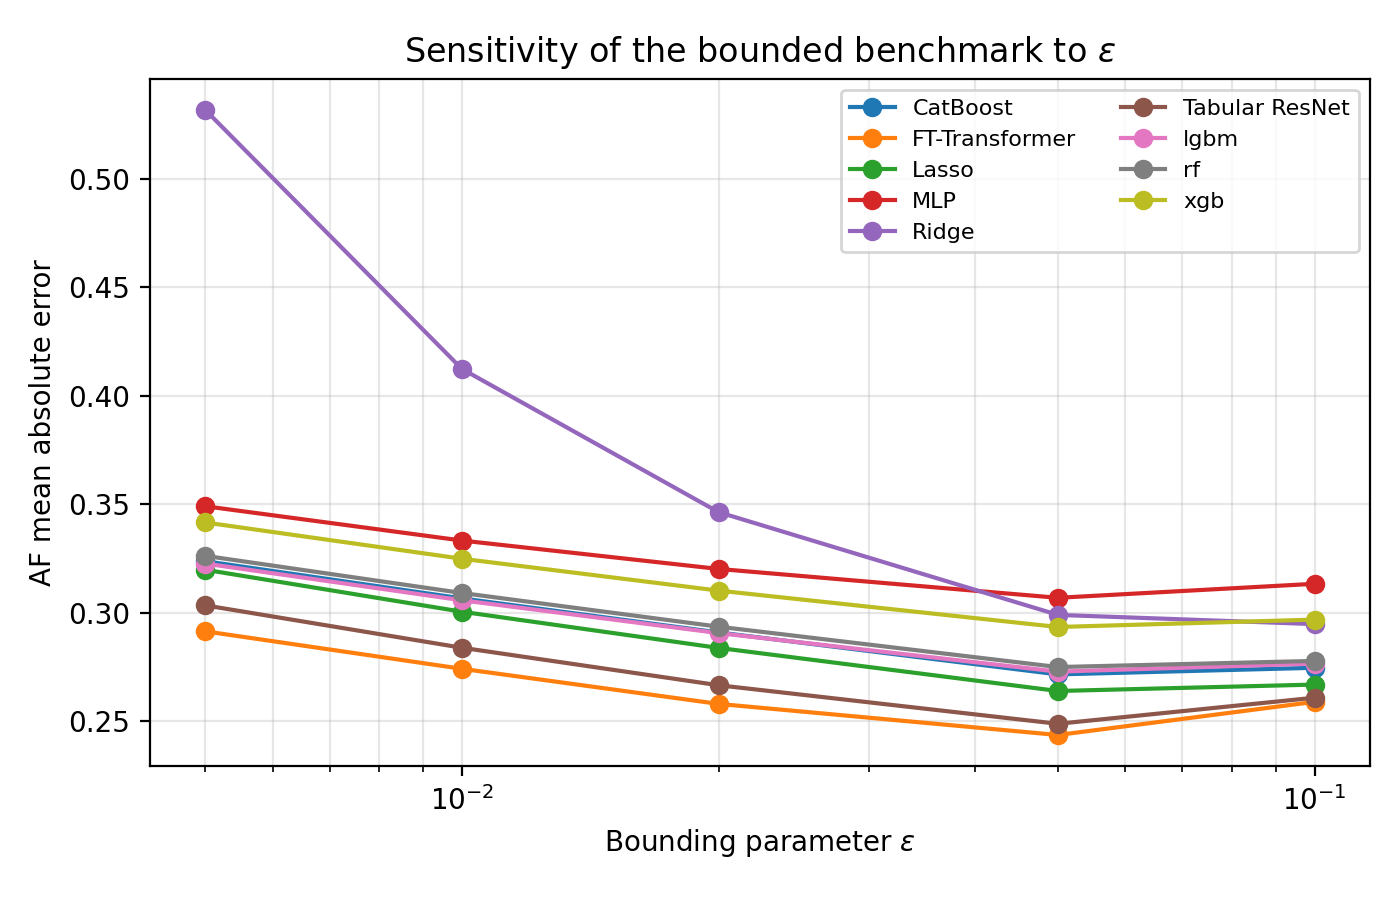
\includegraphics[width=0.85\linewidth]{figA6_eps_sensitivity.png}
\caption{Sensitivity of adjustment-factor mean absolute error to the bounding parameter $\varepsilon$, by model. The horizontal axis uses a log scale because $\varepsilon$ is varied multiplicatively from 0.005 to 0.10.}
\label{fig:eps_sensitivity}
\end{figure}

\section{Estimator details}
\label{app:estimators}
\setcounter{equation}{0}
\renewcommand{\theequation}{B.\arabic{equation}}

This appendix states the estimating equations for the four model families compared in the unified benchmark.


The regularized linear models provide a transparent baseline for the bounded prediction problem. Ridge and Lasso solve
\begin{equation}
\hat{\beta} \;=\; \arg\min_\beta \sum_{i=1}^{n}\bigl(r_i - x_i'\beta\bigr)^2 + \lambda\,\Omega(\beta),
\label{eq:penalized}
\end{equation}
where $\Omega(\beta)=\|\beta\|_2^2$ for ridge and $\Omega(\beta)=\|\beta\|_1$ for lasso \citep{Hoerl1970Ridge, Tibshirani1996}. Fractional logit estimates
\begin{equation}
\mathbb{E}[r_i \mid x_i] \;=\; \Lambda(x_i'\beta), \qquad \Lambda(z)=\frac{\exp(z)}{1+\exp(z)},
\label{eq:fraclogit}
\end{equation}
by quasi-maximum likelihood \citep{PapkeWooldridge1996}. This model is especially useful as a disciplined bounded-outcome benchmark.

Tree-based ensembles allow the conditional mean of the at-home ratio to vary nonlinearly with income, urbanization, prices, and production structure. Boosting-style models approximate the prediction function as an additive collection of regression trees:
\begin{equation}
\hat{r}(x_i) \;=\; \sum_{m=1}^{M}\nu\,f_m(x_i),
\label{eq:boost}
\end{equation}
where each $f_m(\cdot)$ is a tree and $\nu$ is a shrinkage parameter \citep{Breiman2001, ChenGuestrin2016, KeEtAl2017, ProkhorenkovaEtAl2018}.

The preferred FT-Transformer is included because the measurement task involves interactions among household and province-year features. The tokenizer maps each numerical feature $x_{ij}$ into a feature-specific token,
\begin{equation}
t_{ij} \;=\; w_j x_{ij} + b_j,
\label{eq:token}
\end{equation}
while the province identifier is mapped into a categorical embedding. Stacking all tokens gives $Z_i^{(0)}$. Transformer layers update this representation as
\begin{equation}
Z_i^{(\ell)} \;=\; \mathrm{TransformerLayer}_\ell\!\bigl(Z_i^{(\ell-1)}\bigr), \qquad \ell=1,\dots,L.
\label{eq:transformer}
\end{equation}
The bounded prediction is obtained from a sigmoid output layer,
\begin{equation}
\hat{r}_i \;=\; \sigma\!\Bigl(w_o^\top \mathrm{LN}\bigl(\bar{Z}_i^{(L)}\bigr) + b_o\Bigr),
\label{eq:ftout}
\end{equation}
where $\sigma(\cdot)$ is the logistic function, $\bar{Z}_i^{(L)}$ is the mean-pooled token representation, and LN denotes layer normalization \citep{GoodfellowEtAl2016, GorishniyEtAl2021, RubachevEtAl2024}. The baseline uses three encoder layers, 64-dimensional tokens, four attention heads, dropout of 0.1, AdamW optimization, and early stopping.


\end{document}
% =====================================================================
